%!TEX encoding = UTF-8 Unicode
%!TEX program = xelatex

\documentclass[doctor]{ustcthesis}
% bachelor|master|doctor
\usepackage{ustcextra}
\usepackage{diagbox}
\usepackage[tight]{subfigure}
\usepackage{multirow}
\graphicspath{{figures/}}
%\bibliographystyle{ustcauthoryear}

\usepackage{enumerate}
\usepackage{bm}

\def \a {\mathbf{a}}
\def \b {\mathbf{b}}
\def \c {\mathbf{c}} \def \f    {\mathbf{f}}
\def \g  {\mathbf{g}}
\def \h  {\mathbf{h}}
\def \l  {\mathbf{l}}
\def \gt {\mathbf{g}_t}
\def \hy   {\widehat{y}}
\def \m {\mathbf{m}}
\def \p {\mathbf{p}}
\def \q {\mathbf{q}}
\def \ty   {\widetilde{y}}
\def \bu    {\mathbf{u}}
\def \t {\mathbf{t}}
\def \u {\mathbf{u}}
\def \v {\mathbf{v}}
\def \w  {\mathbf{w}}
\def \x {\mathbf{x}}
\def \y {\mathbf{y}}
\def \z {\mathbf{z}}
\def \vpsi {\boldsymbol{\psi}}
\def \zero {\mathbf{0}}
\def \one {\mathbf{1}}
\def \valpha {\boldsymbol{\alpha}}
\DeclareMathOperator*{\argmax}{arg\,max}
\DeclareMathOperator*{\argmin}{arg\,min}

\def \R {\mathbb{R}}

\def \C {\mathcal{C}}
\def \D {\mathcal{D}}
\def \E {\mathcal{E}}
\def \G {\mathcal{G}}
\def \Mu {\pmb{\mu}}
\def \Nn {\mathcal{N}}
\def \H {\mathcal{H}}
\def \L {\mathcal{L}}
\def \U {\mathcal{U}}
\def \S {\mathcal{S}}
\def \X {\mathcal{X}}
\def \Y {\mathcal{Y}}

\def \diag{\mathrm{diag}}
\def \prox {\mathrm{prox}}
\def \det  {\mathrm{det}}
\def \Tr   {\mathrm{Tr}}
\def \Pr   {\mathrm{Pr}}
\def \P   {\mathrm{P}}
\def \DKL   {\mathrm{D_{KL}}}
\def \sign {\mathrm{sign}}
\def \sgn {\mbox{sgn}}
\def \Truncate {\mbox{Truncate}}
\def \trunc {\mbox{trunc}}

\newcommand{\dataset}{{\cal D}}
\newcommand{\includeMyGraphicX}[1]{\includegraphics[clip=true, height=0.32\textwidth, width=0.48\textwidth]{#1}}
\newcommand{\includeMyGraphicY}[1]{\includegraphics[clip=true, height=0.28\textwidth, width=0.48\textwidth]{#1}}


\title{社交多媒体数据\\语义理解和关联表达}
\author{吴岳}
\major{信号与信息处理}
\advisor{俞能海\ 教授\ 李世鹏\ 教授}
%\coadvisor{}
\submitdate{二〇一七年五月}
%\secrettext{机密\quad 小于等于20年}   % 内部|秘密|机密,注释本行则不保密
\depart{电子工程与信息科学系}

\entitle{Social Media Data\\Semantic Understanding and Associative Expression}
\enauthor{Yue Wu}
\enmajor{Information and Communication Engineering}
\enadvisor{Prof.\ Nenghai\ Yu \ Prof.\ Shipeng\ Li}

\encoadvisor{Prof. Shipeng Li}
\ensubmitdate{May, 2017}
%\ensecrettext{Confidential\quad Less than or equal to 20 years}  % Internal|Secret|Confidential

\begin{document}

\maketitle

%
% 本科论文:
%   frontmatter: 致谢、目录、中文摘要、英文摘要
%   mainmatter: 正文章节、参考文献
%   appendix: 附录
%
% 硕博论文:
%   frontmatter: 中文摘要、英文摘要、目录、符号说明
%   mainmatter: 正文、参考文献
%   appendix: 附录
%   backmatter: 致谢、发表论文
%

\frontmatter

\begin{abstract}
    近年来,智能手机及其它移动智能设备呈现出了爆发式的增长与普及。
    高清摄像头、大容量存储和高速的网络连接为用户创造了极其便利的拍摄和分享条件,
    用户几乎可以在任意时间、任意地点拍摄照片或视频,
    并将它们分享到社交网络,产生了海量的社交多媒体数据。
    然而,这些数据都以碎片化的形式存在,当前的社交多媒体系统
    缺乏智能的工具或服务将它们组织起来,并选取符合用户个性化需求的数据呈现给用户,
    用户也很难快速准确地检索到他们需要的数据。
    因此,如何充分挖掘和利用社交多媒体数据成为了当前重要的研究问题。

    本论文对社交多媒体数据的语义理解和关联表达做了深入研究,目标是实现一个能够理解社交
    多媒体数据、根据用户需求选取有关联的数据、并以丰富的表达形式呈现给用户的关联表达系统。
    由于社交多媒体数据的语义内容丰富多样,对每个语义收集并标注数据的难度和成本很高,
    语义理解首先需要解决标注难的问题。 其次,由于社交多媒体数据的规模庞大,
    语义理解需要解决处理慢的问题。
    社交多媒体数据的关联表达是基于对社交多媒体数据语义理解的结果,
    根据用户个性化的需求选取有关联的数据,并以丰富的表达形式呈现给用户。
    本论文分别从照片和视频两个角度研究了关联表达的具体应用。
    语义理解和关联表达构成了挖掘和利用社交多媒体数据相对完整的框架。

    \vspace{0.5em}
    针对上述问题,本论文的主要研究工作和创新成果包括:
    \vspace{-0.5em}
    \begin{enumerate}\setlength{\itemsep}{-0.4em}
        \item 对于语义理解标注难的问题,提出了一种直接从社交多媒体数据学习语义理解模型
            的弱监督相关反馈深度学习算法。传统深度学习算法对于训练数据中的标注噪音十分敏感,
            本论文基于感知连续性,利用数据在特征空间的相互关系,
            使得不同数据在训练过程中有不同的贡献加权, 从而抑制噪音标注的影响。
            实验结果表明,与已有算法相比,本论文提出的弱监督相关反馈深度学习算法具有更好的噪声鲁棒性。
        \item 对于语义理解处理慢的问题,提出了一种从大规模高维数据中选取特征的高效算法。
            本论文基于二阶在线学习算法,利用特征的置信度进行特征选取,
            并利用最大/最小堆结构提出了快速在线特征选取算法。
            由于置信度的单调递增特性,本论文进一步改进了快速二阶在线特征选取算法,
            将算法的复杂度降低为于非零特征数目成正比。
            实验结果表明,该算法能够极大减少特征选取的计算时间,
            并达到当前最好特征选取算法的准确率。
        \item 对于语义理解处理慢的问题,提出了基于二阶在线特征选取算法的
            深度卷积神经网络模型简化算法。
            算法增加了对应卷积层输出特征图每个通道的权重层,并在权重层上进行特征选取,
            从而将三维卷积核的组稀疏优化问题转化为一维特征选取问题。
            实验结果表明,该模型简化算法在不损失模型准确率的情况下极大减少了模型的参数个数。
        \item 对于照片关联表达问题, 提出了一个基于主题的照片集故事化表达系统——Monet。
            系统首先根据照片的时间和位置信息对照片集进行事件检测。
            其次,根据照片的质量、多样性和均衡性选取一部分代表性的图片。
            然后,系统利用弱监督深度学习算法对代表性照片进行内容表征,
            并利用在线特征选取算法选取最能代表照片内容的特征子集。
            系统根据照片的特征赋予不同照片不同的主题。
            最后,系统运用可计算的视频编辑语法对照片进行动画特效处理
            以及音乐的匹配,生成具有关联表达能力的不同主题的视频。
        \item 对于视频关联表达问题,提出了全自动移动多摄像头视频自动剪辑系统——MoVieUp。
            本论文从音频剪辑和视频剪辑两个角度解决自动剪辑问题。
            音频剪辑对音频流进行质量评估,
            在最少切换次数准则下选取高质量的音频流片段,并拼接成单一音频流。
            视频剪辑首先根据音频的节奏以及语义特性选取镜头切换点。
            其次,系统对多摄像头视频进行语义分割,得到子镜头,
            并评估子镜头的视觉质量、相机运动以及相互之间的多样性,
            最终在保证镜头运动一致性的条件下最大化镜头质量和多样性,完成镜头选取,
            并拼接镜头得到单一视频流。
            系统最后对剪辑后的单一音频流和单一视频流进行混流,得到最终剪辑好的视频呈现给用户。
    \end{enumerate}

    \keywords{弱监督深度学习\zhspace{} 特征选取\zhspace{} 模型简化\zhspace{} 照片集故事化表达\zhspace{} 视频自动剪辑}
\end{abstract}

\begin{enabstract}
    The recent years have witnessed the explosive growth and ubiquity of mobile
    smart devices. The high resolution cameras, large storage, and high speed
    network connection of mobile devices have founded the superior conditions
    for capturing and sharing. Users can capture and share photos or videos at
    almost anytime and anywhere.  Up to now, the scale of social media data has
    increased to a huge scale.  However, these data exist in a fragmented way on
    social media, lacking intelligent services to organize them. Neither can
    social media provide data according to personalized user needs, nor can
    users search for their required data efficiently and effectively. As a
    result, how to exploit and utilize the large scale social media data has
    become an important problem.

    This dissertation probes into the semantic understanding and associative
    expression of social media data. The aim is to implement an intelligent
    system that can understand, select, and express social media data in an
    associative way. Due to the wide range of semantics, it's hard to collect
    and label data for every semantic tag. Semantic understanding should solve
    the difficulty of labeling. Besides, accelerating the processing speed  is
    essential due to the large scale of social media data.  Based on the
    semantic understanding, this dissertation studies associative expression
    from photo and video aspects.  Semantic understanding and associative
    expression compose a relatively complete framework for mining and utilizing
    social media data.

    \vspace{0.5em}
    This dissertation conducts deep research on social media data semantic
    understanding and associative expression related problems with the following achievements:
    \vspace{-0.5em}
    \begin{enumerate}\setlength{\itemsep}{-0.5em}
        \item For the difficulty of labeling, we propose a weakly supervised
            relevance feedback deep learning algorithm to learn from
            weakly labeled social media data directly.  Traditional deep
            learning algorithms are sensitive to label noises.
            Our algorithm utilizes the perceptual consistency to
            attenuate the sensitiveness, which uses the correlation in the
            feature space to make different samples contribute differently
            during training.  Empirical evaluation with comparison to existing
            algorithms shows that the relevance feedback algorithm has better
            robustness to label noises.
        \item For the processing speed, we propose a large scale high
            dimensional second-order online feature selection algorithm. Based
            on second-order online learning algorithms, the algorithm selects features
            according to the confidence of features. We propose fast algorithms
            with the Max/Min heap. Due to the monotonous increasing property of
            confidence, we further reduce the complexity of the proposed
            algorithm to be linear to the number of non-zero features.
            Empirical evaluation shows that the algorithm can significantly reduce the training
            time while achieving comparable accuracy to state-of-the-art feature selection
            algorithms.
        \item For the processing speed, we also propose a model simplification algorithm for
            deep convolutional neural networks based on online feature selection.
            The algorithm adds a weighting layer corresponding to each channel of the output
            feature maps of convolutional layers.  The group sparsity problem on the
            three dimensional convolutional kernels is then transformed into the online feature
            selection problem on the one dimensional weighting vector.  Empirical evaluation shows that
            model parameters are reduced significantly with little impact on the accuracy.
        \item For associative photo expression, we propose a theme-based
            photo storytelling system---Monet. First, the system detects events in
            photos according to the time and location information. It then selects
            a representative photo subset according to photo quality, diversity, and
            uniformity. After that, the system uses the weakly supervised relevance feedback
            algorithm to analyze the content of the representative photos.
            Online feature selection algorithm is applied to extract the most distinctive
            features. Based on the features, each photo is assigned with a theme.
            Finally, a fancy video with animation and motion effects is generated and aligned with a music
            according to the computational filming grammars of each theme.
        \item For associative video expression, we propose an automatic mobile
            multi-camera video mashup system---MoVieUp. We solve the mashup problem from audio and video aspects.
            For audio mashup, the system assesses audio quality,
            selects high quality audio segments, and stitches them into a single audio stream. For video
            mashup, the system detects the switching points according to the tempo
            and semantics of audio.  After that, videos are structured into
            subshots. The system evaluates the quality, motion, and diversity
            of the subshots.
            Video shots are selected by maximizing the quality and diversity
            under the constraint of motion consistency.
            Finally,the system multiplexes the audio and video streams to
            generate the well-edited video.
    \end{enumerate}

    \enkeywords{weakly supervised deep learning, feature selection, model simplification, photo storytelling, video mashup}
\end{enabstract}


\tableofcontents
\listoffigures
\listoftables
\listofalgorithms  % 算法索引,如不需要,可直接注释掉本行
% \begin{notation}

\centering
\begin{tabular}{rl}
$\ln x$ & natural logarithm $\log_ex$ \\
$\log x$ & common logarithm $\log_{10}x$ \\
$x\ \mathrm{mod}\ y$ & remainder \\
\end{tabular}

\end{notation}


\mainmatter
\chapter{绪论}
本章首先介绍社交多媒体数据的含义以及社交多媒体数据的研究背景和意义,
并由此引出社交多媒体数据的研究中存在的关键问题,然后介绍本论文的主要工作及创新点,
最后介绍全文的结构安排。

\section{研究背景和意义}
近年来,智能手机及其它智能移动设备呈现出了爆发式的增长与普及。
高清摄像头、大容量存储和高速的网络连接为用户创造了极其便利的拍摄和分享条件,
从而创造了海量的多媒体数据。用户几乎可以在任意时间、任意地点拍摄照片或者视频,
并将它们分享到社交网络。 据统计, 截止到2014年产生了大约$2.7$万亿的用户照片。
到2017年,该数字将会增长到约$4.9$万亿~\cite{phototrend}。
这类由用户产生的多媒体数据具有明显的社交性特点:
\begin{enumerate}\setlength{\itemsep}{0pt}
    \item 用户通常在社交活动中拍摄照片或者视频,同一时间段内同一事件中的其他用户也会拍摄与之相关的内容;
    \item 大量拍摄的照片和视频被用户分享到Flickr、Instagram、YouTube、美拍、优酷等社交网站,
        这些数据包含的时间、地点、内容等信息与其他用户分享的多媒体数据产生关联。
\end{enumerate}
因此,本文将这类用户多媒体数据称为\textbf{社交多媒体数据}。

然而,由于缺乏智能的社交多媒体数据语义理解和关联表达服务,这些海量的数据所包含的信息并没有得到
充分的挖掘和利用。如图~\ref{fig:status}所示,一方面,用户、拍摄设备以及社交多媒体数据的规模
都呈现出并保持着爆发式的增长趋势;
另一方面,这些记录了珍贵记忆的用户数据被大量的存储在本地或者云端磁盘上,
却很少再次被用户浏览和利用。海量的社交多媒体数据并没有带来更好的用户体验。
随着人们对于多媒体的内容品质和个性化需求的提高,越来越多的研究人员和工业界研究机
构投入更多的精力到社交多媒体数据中。

\begin{figure}[ht]
\centering
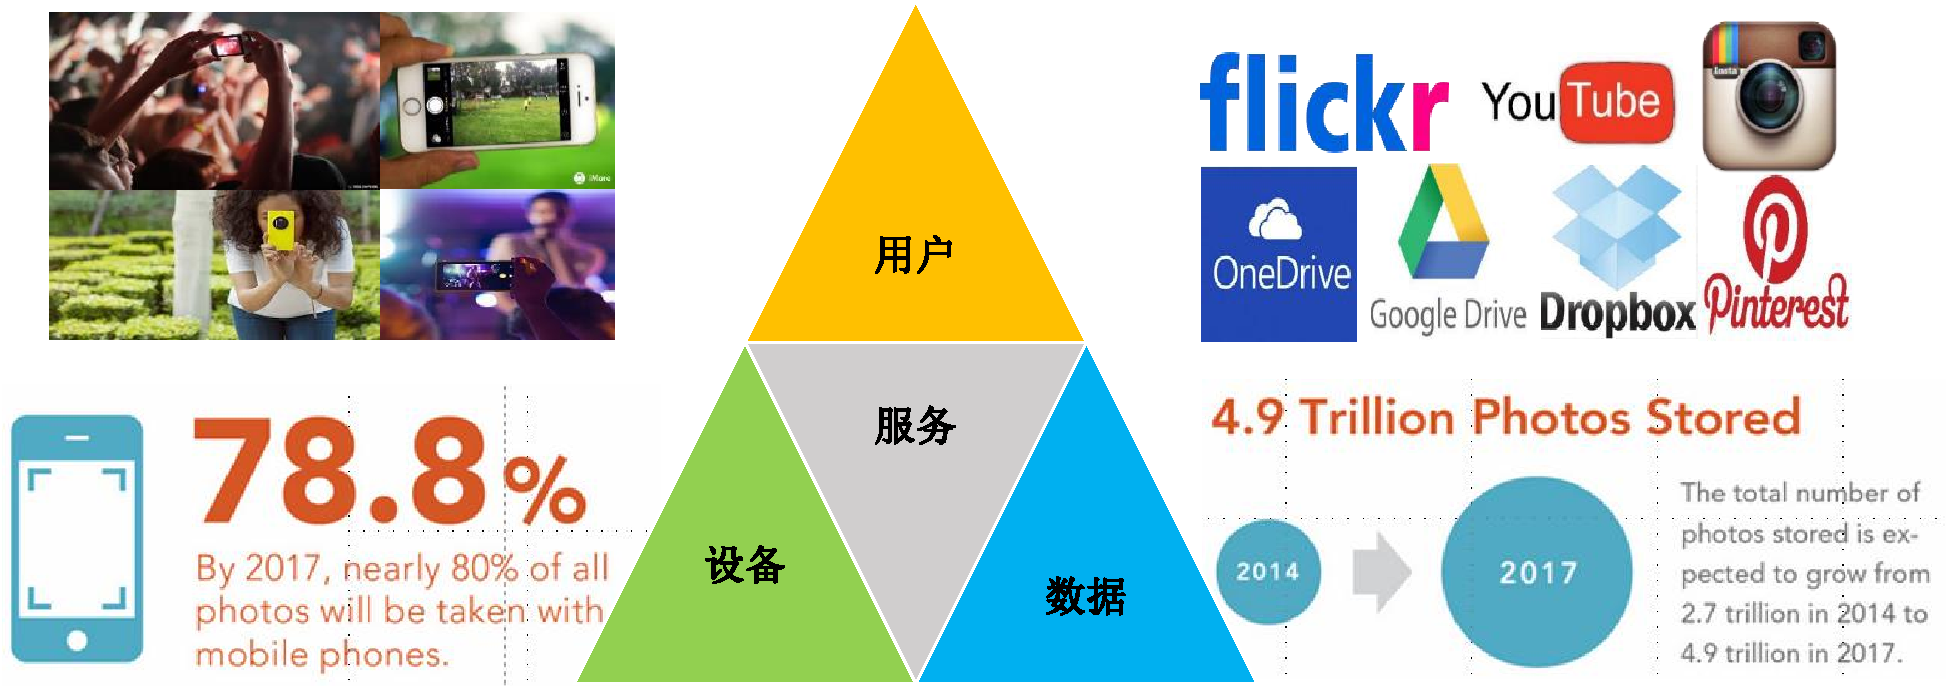
\includegraphics[width=1\textwidth]{social-media.pdf}
\caption{社交多媒体数据产生和利用现状} \label{fig:status}
\end{figure}

相比于传统多媒体数据,社交多媒体数据具有以下特点:
\vspace{-0.2em}
\begin{enumerate}\setlength{\itemsep}{0pt}
    \item \textbf{质量不确定}。由于普通用户的拍摄技巧比较业余、
        拍摄时的光线限制、相机的快速移动或者抖动、场景快速变换等原因,
        社交多媒体数据通常伴有抖动、散焦、过度曝光、欠曝光、模糊、遮挡以
        及拍摄出无意义的照片或视频等问题,影响了社交多媒体数据的后期浏览体验。
    \item \textbf{内容冗余}。用户在拍照时通常采取多次拍摄的方式来获得最理想的拍照效果,
        使得社交多媒体数据中存在大量冗余。这些冗余数据带来三个方面的主要问题:
        (1)需要耗费大量的时间和精力去整理;(2)占据了大量的存储资源;
        (3)增加了用户查找数据的难度。
    \item \textbf{多样性}。用户拍摄的时间、地点和环境比较随机,拍摄的角度、
        内容具有很大的不确定性,使得社交多媒体数据的内容表现出多样化的特点。
        社交多媒体数据相关的服务,不仅需要去除冗余的用户数据,
        也需要最大程度的保留用户数据的多样性。
    \item \textbf{故事性}。用户的拍摄行为并不是随机的,而是选择性地记录对他们有意义的时刻和场景。
        相同时间段内相近地点拍摄的多媒体数据,浓缩了用户在一段时间内的足迹以及经历的事件。
        完整的多媒体数据则记录了很长一段时间内发生在用户身上的故事。
        然而,当前社交多媒体数据相应的服务还不能很好地将这些原始的记录片段整理成高观赏性的纪录片。
    \item \textbf{具有位置和时间信息}。现代移动设备拍摄时通常都能检测到拍摄的时间、地点等信息,
        并将这些信息存储在图像或者视频的文件头中。这些时间和地点信息记录了拍摄的时空上下文关系,
        使得数据之间能够产生关联。基于用户历史拍摄的时间、地点和具体内容,可以更好地挖掘出
        发生在用户身上的故事。
\end{enumerate}

社交多媒体数据具有数量庞大、质量不确定、内容冗余、多样、带有丰富的故事性和时空上下文信息等特点,
对相关的处理算法提出了更高更复杂的要求。因此,对于社交多媒体数据的研究已经成为计算机视觉领域的热点问题,
相关的成果不仅有利于推动计算机视觉以及多媒体领域相关课题的创新,
对于用户体验的提升以及工业界的发展也具有重要的应用价值和现实意义。

\section{社交多媒体数据研究的关键问题}
\label{sec:key_problems}
社交多媒体数据的研究涉及图~\ref{fig:key-problems}所示内容分析层的语义理解和应用层的关联表达两个大的方面。
\begin{figure}[ht]
\centering
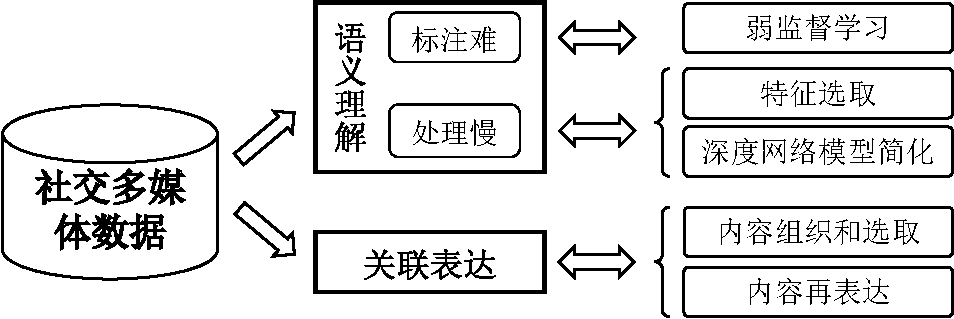
\includegraphics[width=0.9\textwidth]{key-problems.pdf}
\caption{社交多媒体数据研究的关键问题}
\label{fig:key-problems}
\end{figure}

其中,语义理解面临的主要问题包括:
\begin{itemize}
    \item 标注难的问题。机器学习算法可以归纳为有监督学习、半监督学习和无监督学习三个类别。
        有监督学习通常能够获得最好的学习效果。然而,它依赖大量准确的标注数据,
        在当前大数据的背景下有监督学习的应用成本十分高昂。
        据了解,目前最大的有标注图片数据集ImageNet~\cite{russakovsky2015imagenet}
        花费了大约$25,000$名用户一年左右的时间完成标注。
        尽管如此,ImageNet仅包含$22,000$个类别,与现实应用中的语料库相差甚远(如WordNet
        ~\footnote{\url{http://wordnet.princeton.edu/}})。
        与之相反,半监督学习和无监督学习不需要大量的标注数据,但是学习的效果与有监督学习
        还有明显的差距。 基于以上问题,
        越来越多的研究人员将注意力投向了弱监督学习上(Weakly Supervised Learning)。
        弱监督学习是指从标注不完备、不准确的噪音数据中,
        充分挖掘有价值的信息,滤除或抑制错误信息,达到学习模型的目的。
        因此,弱监督学习能够充分利用有噪音的标注数据,
        解决有监督学习标注难和无监督学习效果差的问题。
    \item 处理慢的问题。社交多媒体数据的规模十分庞大,
        对于模型的复杂度以及硬件的计算能力都提出了很高的要求。
        此外,移动设备的计算能力、存储空间以及电池容量依然有限,
        提高社交多媒体数据的处理速度对于提升移动端的用户体验也至关重要。
        为了解决处理慢的问题,一方面可以利用特征选取减少特征提取的种类和数目。
        图片和视频的内容既包括传统的全局特征、局部特征,
        也包括近年来提出的深度神经网络产生的特征。
        对于不同的任务,某些特征具有很强的表征能力,某些特征则十分冗余。
        因此,选取对具体任务最紧凑、最具有表征能力的特征作为数据内容的表达,
        既可以减少特征提取的种类和数目,也可以减少后续模型学习的计算量。
        另一方面,可以对特征提取过程中用到的模型进行简化,
        减少每种特征提取的时间开销。例如,近年来深度神经网络在目标识别、
        物体检测等领域取得了非常好的效果,但是网络的深度和参数数目也在不断增加,
        如何在不影响模型准确度的情况下简化深度神经网络成为了当前研究的热点问题。
\end{itemize}

社交多媒体数据关联表达是指根据用户个性化的需求,从社交多媒体数据中选取有关联的数据,
并以一定的表达形式将这些关联数据呈现给用户。它面临的主要问题包括:
\begin{itemize}
    \item 内容组织和选取。当前,社交多媒体数据以碎片化的形式,
        按照用户拍摄或上传的时间顺序存储在云端服务器上,
        社交网站以及搜索引擎根据用户提供的标签对数据进行索引、
        查询和检索。然而,社交多媒体数据存在质量不确定、内容冗余多样以及故事性等
        特点,高效的内容组织和选取需要理解数据之间的关联性和故事性,从时间、位置、
        用户、内容、关联性等多个维度对数据进行组织和选取。
    \item 内容再表达。内容组织和选取是将数据高效地组织在一起,
        并选取最能满足用户需求的数据。在实际应用中,需要在原始社交多媒体数据的基础上以一种新的、富有艺术美感的
        形式将数据重新呈现给用户。例如,Magisto \footnote{\url{http://www.magisto.com}}
        系统能够给用户的照片和视频加上丰富的特效,并将视频和音乐的节奏进行匹配,
        生成类似专业编辑人员编辑的具有丰富表现力的音乐视频。
        专业的编辑人员在视频编辑中根据素材的内容以及需要表达的效果选取与之相适应的
        素材和特效对视频进行编辑。对于计算机,如何将专业编辑人员在编辑中运用到的规则和
        语法转化成可计算的规则和算法是社交多媒体关联表达面临的一个主要问题。
        由于表现形式以及编辑语法的多样性和主观性,挖掘和应用可计算的编辑语法也具有非常大的挑战性。
\end{itemize}

\section{本文主要工作}
针对\ref{sec:key_problems}节中提到的关键问题,本文分别对社交多媒体数据
的语义理解和关联表达做了深入的研究,构成了社交多媒体数据挖掘和利用的一个相对
完整的框架。图~\ref{fig:correlation}给出了本文研究的具体内容以及相互之间的关联。
针对语义理解标注难的问题,弱监督深度学习直接从不准确标注的社交多媒体数据
中学习语义模型,理解数据的内容。结合传统计算机视觉方法和弱监督深度学习得到的
特征,特征选取针对具体的任务选取最紧凑、最有代表性的特征来表征数据内容,
减少特征提取的种类和数目,加快大规模社交多媒体数据处理的速度。此外,弱监督深度学习
需要耗费大量的计算资源,本论文结合特征提取算法,提出了深度卷积神经网路模型简化算法,
减少网络的参数数目和计算时间。对于社交多媒体数据的关联表达,本论文从基于主题的照片集故事化表达和移动多摄像头
视频自动剪辑两个方面做了具体的应用研究。其中,基于主题的照片集故事化表达分析检测照片集中的事件,
根据照片的质量和关联选取有代表性的照片、并通过可计算的视频编辑语法,对照片集
进行故事化的表达。移动多摄像头视频自动剪辑将同一时间段内同一地点不同用户拍摄的
多摄像头视频在时间上进行同步,通过可计算的视频编辑语法选取镜头和录音,
将多摄像头视频剪辑成单一高质量的音视频流。

\begin{figure}[t]
\centering
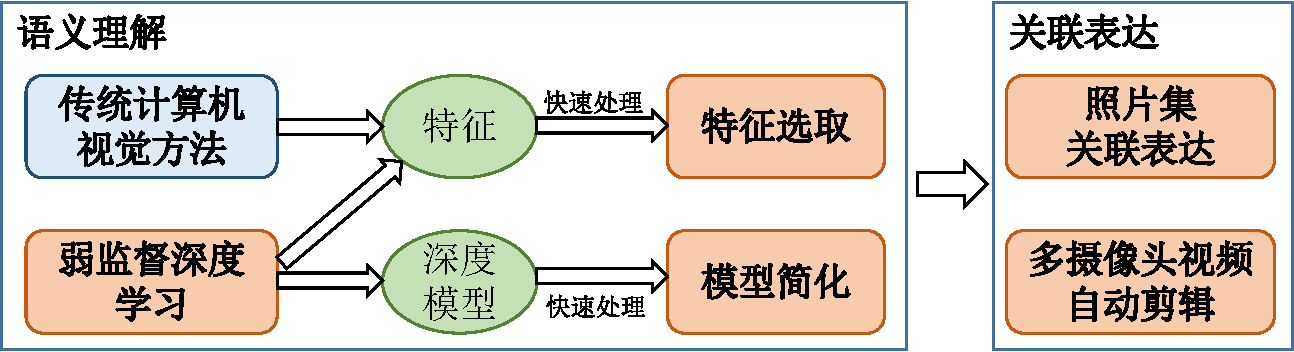
\includegraphics[width=0.9\textwidth]{correlation.pdf}
\caption{社交多媒体数据的研究内容和相互关联}
\label{fig:correlation}
\note{橙色部分表示本论文的研究工作}
\end{figure}

基于以上研究点,本论文具体的研究内容包括:
\vspace{-0.5em}
\begin{enumerate}\setlength{\itemsep}{0pt}
    \item 弱监督深度学习算法研究。 针对任意语义类别,
        从社交多媒体获取弱标注数据,提出具有抗噪效果的语义理解模型。
        传统深度学习算法对于噪声的敏感性是由于所有的数据在学习过程中具有相同的权重。
        本论文提出方法的基本假设是:同一类别下,正确标注的数据由于语义上关联,
        在特征空间上比较接近,而错误标注的数据则与其他数据有很大差异。
        因此,可以利用数据在特征空间上的关系,使得不同数据在训练过程中有不同的贡献加权,
        使得特征空间上的``孤立''数据具有较小的权重,
        特征空间上密集区域的数据具有较大的权重,我们称之为相关反馈。
        该思想可以在学习过程中通过特征空间的低秩近似实现。
        为了加速模型的训练速度,我们进一步对模型进行了简化和近似,降低了模型的复杂度,
        用于学习大规模社交多媒体数据的语义理解模型。
    \item 大规模高维特征选取算法研究。
        多媒体数据的特征表示不仅包括高层次的神经网络特征,
        还包含低层次的全局特征(如颜色特征、纹理特征),局部特征(如SIFT~\cite{lowe1999object}、SURF~\cite{bay2006surf})
        以及通过局部特征描述整体视觉信息的词袋特征等。
        实际应用中需要根据需求选取对目标任务最有用的特征子集,
        这对于大规模社交多媒体数据的处理速度以及移动设备有限的计算能力和内存空间尤其重要。
        此外,去除特定任务不相干的特征,还可以提高特征的表达能力。
        本论文利用二阶在线学习算法,基于特征的置信度进行特征选取,
        并利用最大/最小堆结构提出从大规模高维数据中选取特征的高效算法。
        已有的稀疏在线特征选取算法的复杂度与特征的维度成正比,
        本论文进一步利用置信度的单调递减特性提出了快速二阶在线特征选择算法,
        将算法的复杂度降为与非零特征数目成正比。
    \item 深度卷积神经网络模型简化算法研究。
        深度卷积神经网络的深度和模型参数通常比较大,
        例如经典的VGG16网络包含超过138M的模型参数。
        大量的模型参数意味着在实际应用中需要大量的计算资源和时间,
        极大限制了深度神经网络在大规模社交多媒体数据相关任务上的应用。
        此外,深度网络在移动设备上的应用已经成为一种趋势。由于移动设备计算能力、存储空间和
        电池容量的限制,在不影响模型准确率的条件下简化深度网络模型已经成为迫切的需要。
        本论文提出一种基于在线特征选取的模型简化算法。算法主要针对卷积层进行简化,
        对卷积层输出的e特征图增加对应每个通道的权重层,
        并利用在线特征选取算法对每个通道对应的权重进行更新和选取。
        区别于传统方法,在线特征选取方法可以在训练过程中动态调整需要保留的卷积核,
        减小模型简化对网络性能的影响。

    \item 基于主题的照片集故事化表达算法研究。照片集故事化表达首先对照片集进行事件检测,
        找出用户所拍摄的不同事件,并选取一部分照片子集代表整个照片集。
        其次,利用弱监督深度学习算法进行照片内容分析。由于深度网络的每一层都是对照片不同层次的语义表达,
        本论文利用在线特征选取算法选取最能表征照片语义的特征子集,
        构成照片内容的最终表达。为了达到更好的关联表达效果,不同主题的照片需要采用不同的编辑风格。
        本论文从网络上抓取训练图片,利用弱监督深度神经网络得到主题风格的分类器,为照片集中的照片选取合适的编辑风格。
        最后,通过可计算的视频编辑语法,对照片进行动画特效处理以及音乐的匹配,生成具有关联表达能力的视频呈现给用户。

    \item 移动多摄像头视频自动剪辑算法研究。多摄像头视频是指在同一时间段、同一地点由不同摄像头拍摄的时间上有重叠的
        一组视频。多摄像头视频是不同用户从不同的角度对相同事件的记录。本文提出一个全自动移动多摄像头视频自动剪辑系统。
        我们首先邀请专业的视频编辑人员探讨可计算的视频编辑语法。根据这些语法,自动剪辑系统首先对音频流进行质量评估,
        在保证尽可能减少音频切换次数的条件下选取高质量的音频片段, 形成单一音频流。
        对于视频流,系统首先根据音频的节奏以及语义特性选取视频镜头切换点。
        其次,对多摄像头视频进行语义分割,得到视频子镜头,并对这些子镜头的视觉质量、相机运动以及相互之间的多样性进行评估。
        在保证镜头运动一致性的前提下最大化质量和多样性,选取视频镜头,得到单一视频流。
        单一的音频流和频流通过混流得到剪辑好的视频呈现给用户。
\end{enumerate}

\section{本文主要创新点}
本论文的主要创新有以下几点:
\begin{enumerate}
    \item 针对社交多媒体数据标注难的问题,提出了一种可以从社交多媒体数据中学习目标识别模型的
        弱监督相关反馈深度神经网络学习算法,摆脱了对大量标注数据的依赖。该算法利用数据之间的关联,
        使得不同数据在模型训练中有不同的贡献加权。同时,通过对模型的简化和近似,降低了模型复杂度,
        对于训练大规模社交多媒体数据具有重要意义。
    \item 针对大规模社交多媒体数据处理慢的问题,提出了从大规模高维数据中选取特征的高效算法。
        相比于已有的批处理算法和在线特征选取算法,该算法显著降低了特征选取的时间复杂度,
        并能达到与已有特征选取算法差别不大甚至更好的准确率。
    \item 针对深度网络处理慢、耗费计算资源的问题,提出了简化深度卷积神经网络的高效算法,
        将传统的多维卷积核组稀疏优化问题转化为一维特征选取问题,在不影响模型准确率的情况下极大减少了模型参数。
    \item 提出了基于主题的照片集故事化表达系统——Monet,从照片集中自动检测事件,选取有代表意义的照片,
        选取合适的视频编辑风格,并将可计算的频编辑语法应用到照片集的编辑中。
    \item 提出了移动多摄像头视频自动剪辑系统——MoVieUp,自动剪辑移动多摄像头视频并生成高质量的单一音频视频流。
        该方法首次考虑了音频流的剪辑,并且首次系统地讨论了视频编辑理论在移动多摄像头视频自动剪辑中的应用。
\end{enumerate}

\section{本文结构安排}
本论文主要研究社交多媒体数据语义理解和关联表达中的几个关键问题:弱监督深度学习、
特征选取、模型简化、基于主题的照片集故事化表达和移动多摄像头视频自动剪辑。
各章节内容安排如下:
\begin{itemize}
    \item 第2章从弱监督学习、特征选取、模型简化和关联表达四个方面介绍本论文相关工作的
        研究现状和工作基础。在弱监督学习方面,主要介绍了传统的弱监督学习方法和
        近年来热点研究的弱监督深度学习方法;在特征选取方面,主要回顾了传统的
        批处理方法,用于解决大规模流数据的在线学习方法和在线特征选取算法;
        在模型简化方面,主要介绍与深度神经网络相关的模型简化工作;
        在关联表达方面,主要介绍学术界和工业界关于社交多媒体数据的研究成果
        和代表性应用产品。
    \item 第3章重点介绍弱监督相关反馈深度神经网络的设计思路和实现方法、
        网络模型的简化和近似策略以及相应的实验结果。
    \item 第4章介绍大规模社交多媒体数据快速处理方法,包括在线特征选取的基本模型、
        本文提出的置信度加权二阶在线特征选取方法以及相应的快速算法。
        此外,该部分还介绍深度卷积神经网络模型简化的问题建模和具体算法,以及相应的实验结果。
    \item 第5章介绍基于主题的照片集故事化表达系统,包括照片集的事件检测、代表性照片
        选取以及照片的质量评估、多样性评价和均衡性考量。
        系统为选取的代表性照片上分配不同的主题风格,并利用针对不同风格设计的可计算的编辑语法,
        对照片赋予丰富的特效,生成具有表现力的视频,重现照片集中的场景和故事。
    \item 第6章介绍移动多摄像头视频自动剪辑系统。首先介绍针对移动多摄像头视频
        自动剪辑的可计算的视频编辑语法,并提出相应的系统框架。其次,该部分详细介绍了
        音频的质量评估和剪辑方法、基于音频节奏和语义内容的视频切换点检测算法
        和基于镜头质量、多样性和运动连续性的镜头选取算法。最后,通过实验证明
        了系统各个部分的有效性和整体的用户体验。
    \item 第7章对全文进行总结,并展望未来可以进一步开展和改进的工作。
\end{itemize}


\chapter{国内外研究现状和工作基础}
本章对社交多媒体数据语义理解和关联表达涉及的关键问题的研究现状和工作基础做详细回顾。
首先回顾弱监督学习,总结近年来弱监督学习和弱监督深度神经网络的发展情况;
然后针对社交多媒体数据的特征选取, 回顾传统的批处理方法、
解决大规模流数据的在线学习方法、在线特征提取算法以及它们在
解决大规模社交多媒体数据特征选取问题中的不足;
在模型简化方面,主要介绍与深度神经网络相关的模型简化工作;
对于关联表达,本章从照片集和移动多摄像头视频两个角度分别介绍学术界和工业界
的研究成果和代表性应用产品,指出它们在社交多媒体数据关联表达中
的不足,引出本论文提出的基于主题的照片集故事化表达系统和移动多摄像头视频自动剪辑系统。

\section{弱监督学习}
弱监督学习是指训练数据标注不完备或包含噪音条件下的学习问题。本论文主要针对
弱监督目标识别问题做工作总结和算法创新。具体的方法可以分为两个方面:
数据去噪和噪音鲁棒模型。

\subsection{数据去噪}
\label{sec:data-cleaning}
数据去噪是指找出并移除可能错误标注的数据。
数据去噪的优点在于不依赖目标任务的模型和训练方法,
但同时也面临区别噪音数据和异常数据的难题~\cite{danyluk2014small}。
数据去噪方法会导致两种类型的错误:正确标注的样本被误判为错误标注并被丢弃,
以及错误标注的样本被漏判。

经典的数据去噪方法基于从数据本身提取的特征进行判别。
Brodley等人提出的交叉过滤法~\cite{brodley1999identifying}采用类似于交叉验证的思路,
将训练数据分成$n$等份, 并选择$m$种分类算法(称为过滤算法)。 对于每份数据,
在剩下的$n-1$份数据上训练$m$个分类模型,然后用得到的$m$个分类器对这部分数据进行预测,
最后判定错误标注的数据并将之移除。
此外,Zhou等人提出的最大边界难分类样本学习算法迭代地学习正负类别分界面,
保留难分类数据,移除易分类数据,通过更新正负样本集的方法
达到去除噪音数据的目的~\cite{zhou2015conceptlearner}。

交叉过滤法和最大边界难分类样本学习算法属于有监督学习方法。
研究人员也提出了半监督噪音数据去除方法——核平均算法~\cite{huang2006correcting,vo2015deep}。
半监督学习方法首先人工标注部分数据作为种子数据,记为$\L = \{(\x_i, y_i)\}_{i=1}^m$。
剩余数据记为$\U = \{\z_j\}_{j=1}^n$。通常情况下,$m \ll n$。
核平均算法的核心思想是对未标注的数据加权,
使得加权后未标注数据的分布与有标注数据的分布相同。

此外,社交多媒体数据具有丰富的上下文信息,
这些上下文信息从侧面反映了数据内容, 因此可以用来辅助数据去噪。
Schroff等人提出了一种基于图片上下文信息进行重排序的算法~\cite{schroff2011harvesting}。
算法首先利用图片附近的文本上下文学习标注是否正确的后验概率并进行重排序,
然后从基于文本重排序的结果中选择前$n_+$个图片作为正样本,
再从所有其他类别的图片中选择$n_-$个图片作为负样本,再对图片提取视觉特征,
训练SVM分类器。社交主动学习(Social Active Learning)首先用视觉特征训练
分类器,并评价数据对于提升分类效果的信息量,同时利用文本特征评价每个数据标注可靠
的置信度,综合考虑信息量和置信度选取数据,
迭代地训练模型并选取正确标注的数据~\cite{chatzilarisalic}。

可以看出,数据去噪方法分成两步进行:特征提取和数据去噪的模型训练,
对于噪声的判别也依赖于人为假设和定义的准则,这些因素导致在真实的
社交多媒体数据上,数据去噪方法的效果受多重因素影响,很难达到理想的效果。

\subsection{噪音鲁棒模型}
噪音鲁棒模型是指对数据的标注噪音不敏感或具有抑制作用的模型。
在经验风险最小化(Empirical Risk Minimization, ERM)规则和特定的损失函数下,
如果模型发生分类错误的概率保持不变并且与标注噪音无关,
则认为模型是对标注噪音鲁棒的。研究人员讨论了在特定条件下,理论上是否存在
对标注噪音完全鲁棒的模型~\cite{manwani2013noise}。 例如,
$0-1$损失函数在均匀标注噪音或者能达到$0$错误率的情况下是
噪音鲁棒的~\cite{thathachar2011networks,sastry2010team}。
Beigman等人讨论了非随机噪音模型下的鲁棒模型~\cite{beigman2009learning},
最小平方差损失函数在均匀标注噪音下同样是噪音鲁棒的。其它常见的损失函数,如
指数损失函数,对数损失函数,以及Hinge Loss都不是噪音鲁棒的。换句话说,大部分常见的
机器学习算法都不是完全噪音鲁棒的,但可以在一定程度上减小错误标注的影响, 提升
模型的鲁棒性。

对于经典的SVM分类器,Bunescu等人提出了稀疏多实例学习算法用于解决训练样本中的
噪音数据问题~\cite{bunescu2007multiple,vijayanarasimhan2008keywords}。
多实例学习将一组包含正样本的有噪音数据称为一个正样本包,将一组负样本数据称为负样本包,同时假设正样本包
中至少包含一个真实的正样本,负样本包中全是负样本。通过对正负样本包采用
不同的约束条件和惩罚系数,达到抑制噪音影响的目的。

直推式支持向量机(Transductive Support Vector Machine, TSVM)
~\cite{sindhwani2006large,vo2015deep}是一种半监督学习算法,
该算法同时根据有标注的数据$\L$和未标注的数据$\U$寻找分界面,
并约束最多有$r$个未标注数据被判定为正样本来抑制噪音数据的影响。

逻辑回归是一种经典的概率统计分类模型,得到了十分广泛的应用。
然而,逻辑回归算法对于训练数据中的标注噪音十分敏感。
Feng等人提出了一种基于次高斯分布的鲁棒逻辑回归算法~\cite{feng2014robust}。
根据理论分析结果,算法首先去除范数大于一定阈值的数据,
在剩余数据中仅最大化前$n_1$个数据的标注和预测结果之间的相关度。
此外,在随机噪音(Noise at Random, NAR)假设下,研究人员提出用隐藏变量对数据的真实类别、错误标注的转移概率
以及测到的标注建模,并通过EM算法优化目标结果~\cite{izadinia2014image,izadinia2015deep}。

近年来,深度卷积神经网络在目标识别上获得了巨大的成功。
卷积神经网络最早于1998年被Lecun等人应用在文字识别上~\cite{lecun1998gradient}。
得益于显卡设备的快速发展,卷积神经网络的深度、宽度以及结构不断改进,
深度卷积神经网络的识别能力和应用范围都得到了巨大的
提升~\cite{krizhevsky2012imagenet,simonyan2014very,szegedy2015going,szegedy2016rethinking,szegedy2016inception,he2016deep}。

然而,深度卷积神经网络需要大量的训练数据,对于数据标注的准确性有很大依赖。
如何利用容易获得的弱监督数据训练深度卷积神经网络成为了近年来的研究热点之一。
自举深度神经网络是2014年谷歌研究团队提出的利用图片特征之间的相似性
监督网络学习、抑制错误标注影响的学习方法~\cite{reed2014training}。文章
认为,如果图片的特征之间具有相似性,预测的结果也应该比较相似。
这种相似性被称之为感知连续性。在随机噪声的假设下,该方法在神经网络中加入全连接隐藏层表示真实的
类别。为了达到感知连续性的约束,论文提出引入类自适应编码器的方法训练网络。此外,还可以
通过约束隐藏层输出的熵最小达到软自举优化,
以及约束隐藏层概率最大类别的熵最小达到硬自举优化。Sukhbaatar等人通过约束
隐藏层参数的迹达到感知连续性的优化目标~\cite{sukhbaatar2014training}。
Xiao等人综合考虑了标注可能遇到的随机噪音和非随机噪音,通过隐藏变量对不同噪音
类型下的概率建模,用两个神经网络分别学习噪音类型和真实的标注,通过EM算法
学习整个模型的参数~\cite{xiao2015learning}。 以上方法都基于特定的噪音模型。
Azadi等人提出一种辅助图片正则项(Auxiliary Image Regularizer, AIR)方法~\cite{azadi2015auxiliary},
根据数据的特征结构,通过组约束使得只有部分数据具有响应,在训练数据中识别出有用的辅助数据,
从而更好地训练神经网络。某种程度上,可以认为辅助图片正则项方法是在训练数据中寻找最近邻数据,
减少深度模型对噪音数据的拟合。

传统的噪音鲁棒模型仍然基于特征提取和模型训练两个步骤,
具有\ref{sec:data-cleaning}节提到的局限性。现有的弱监督深度学习
方法基于特定的噪音模型,难以处理真实的场景,或建模过于复杂,难以
训练。因此,本论文提出一种新的利用数据在特征空间的相关性作为相关反馈的弱监督深度神经网络,
并对网络进行简化和近似,提高模型的适用性和实用性。

\section{特征选取}
数据的特征表示不仅包括高层次的神经网络特征,还包含低层次全局特征(如颜色特征~\cite{jain1996image}、
边缘特征~\cite{jain1996image} 、纹理特征~\cite{manjunath1996texture})、
局部特征(如SIFT~\cite{lowe1999object} 、SURF~\cite{bay2006surf}),
以及通过局部特征描述整体视觉信息的词袋特征等~\cite{yang2007evaluating}。
实际应用中需要根据需求选取对目标任务最有用的特征子集,
这对于处理大规模社交多媒体数据以及计算能力、内存和电量都十分受限的移动设备尤其重要。
此外,去除特定任务不相干的特征,还可以提高特征的表征能力。
特征选取在机器学习和数据挖掘领域得到了广泛的研究,
从处理数据的方法上可以将特征选取算法分成两大类别:批处理方法和在线特征选取。

\subsection{批处理方法}
批处理方法是指训练过程中每次迭代都需要考虑所有的训练数据,可以分为三个类别:
\begin{itemize}
    \item 过滤法(Filter)。 过滤法分析特征之间的关联、距离、交互信息熵等,
        选取最有代表意义的特征子集~\cite{yu2003feature,jiang2015relative,li2016feature} 。
        Yang等通过分析指出,传统的过滤法存在单调性的问题,
        不同大小的特征子集之间存在单调的包含关系,
        这种包含关系在实际情况中并不成立~\cite{yang2013efficient}。
        他们对特征之间的联系建模,提出了一种多核学习的方法。
    \item 包装法(Wrapper)。包装法使用预先定义的分类器评价特征子集的性能~\cite{kohavi1997wrappers}。
        这类方法迭代地选取不同的子集,并得到该子集在分类器上评价结果,
        虽然包装法能够获得该分类器上最好的特征子集,但计算过程过于复杂,因此对于该类方法的研究相对较少。
    \item 嵌入法(Embedded)。嵌入法将特征选取与模型训练融合,
        是一种综合平衡过滤法的高效率和包装法的高准确性的方案~\cite{pappu2015sparse,le2014feature}。
\end{itemize}

\subsection{在线特征选取}
批处理方法的缺点在于需要将所有训练数据都加载到内存中。
对于大规模高维数据,这类方法的局限性十分明显。
此外,批处理方法假设数据预先已经全部存在,而实际场景中数据大多是流媒体数据。
因此,随着近年来数据量的增大和维度的增加,大量的工作转向了在线学习。
最早的在线学习算法是1958年提出的感知机算法~\cite{rosenblatt1958perceptron}。
2006年,Crammer等人在感知机算法上约束型每次更新后在当前数据上能获得正确的预测结果~\cite{crammer2006online}。
考虑到批处理学习算法中,二阶海森矩阵能够显著提高算法的收敛速度,
Crammer等人假设模型参数服从高斯分布,用协方差矩阵表示当前模型对于参数的不确定性,
提出了置信度加权的在线学习算法~\cite{crammer2009multi}。
该算法每次更新时约束更新后的模型以一定概率在当前的数据上获得正确的预测结果。
自适应的置信度加权在线学习算法在此基础上降低了模型对于数据噪音的敏感性~\cite{crammer2009adaptive}。

在线学习也被应用到特征选取上。Langford等人提出的稀疏在线学习算法
在感知机模型上增加了模型参数的$L1$范数作为正则项,
学习稀疏在线模型~\cite{langford2009sparse}。
Duchi等提出的FOBOS算法将稀疏在线学习分成两步,第一步是传统的在线学习,
第二步是约束模型的$L1$范数同时使得模型尽可能接近第一步得到的参数~\cite{duchi2009efficient}。
另一种稀疏在线学习思路是优化模型在主空间和对偶空间的距离,
利用模型的$L1$范数实现稀疏优化而提出的RDA算法~\cite{xiao2010dual} 。
RDA算法在高稀疏度下往往能获得更好的效果。
受置信度加权等二阶算法的启发,Duchi等利用梯度的协方差矩阵构建二阶信息,
提出了自适应的二阶FOBOS算法和二阶RDA算法~\cite{duchi2011adaptive}。

基于$L1$范数的稀疏在线学习算法是针对特征选取的``软''约束方法。
参数设定与目标特征数目之间没有确定的关联。
基于$L0$范数的在线特征选取也得到了研究人员的关注。
Wu等提出的在线特征流学习算法能够在每次迭代后返回一个模型和它选取的特征子集~\cite{wu2010online}。
该算法每次获得所有数据的某个特征,算法按顺序依次处理所有特征。
另一种更普遍的应用场景下,算法每次获取一个数据的部分或者所有特征,
算法按时序依次处理所有数据。该场景下,Huang等提出一种无监督在线特征选取算法~\cite{huang2015unsupervised}。
Wang等利用有监督的数据,根据权重向量的绝对值在线选取特征~\cite{wang2014online}。

批处理方法的主要问题在于不具有可伸缩性,以及对于流数据不具有很好的应对能力。
基于$L1$范式的稀疏在线学习方法不能直接约束特征数目,
在实际应用中需要根据不同的数据反复调整参数选取预期数目的特征。当前的在线
特征选取算法根据权重向量的绝对值选取特征,其结果与批处理方法还有较大差距,
并且算法的复杂度仍然较高。因此,本论文提出了大规模高维特征选取算法,
不仅显著减小了计算复杂度,还能达到批处理方法相近甚至更好的准确率,
对于处理大规模社交多媒体数据具有非常大的应用价值。

\section{模型简化}
近年来,深度卷积神经网络在目标识别、物体检测等领域获得了巨大的成功。
为了进一步提高网络的表征能力,研究人员不断改进网络的深度~\cite{simonyan2014very}、
宽度~\cite{zagoruyko2016wide}以及拓扑结构~\cite{szegedy2015going,srivastava2015highway,he2016deep}。
然而,大量的网络参数也要求大量的时间开销和计算资源,同时也极大地限制了
深度网络在计算能力、存储空间和电池续航受限的移动设备上的应用。如何在
不影响网络性能的情况下减少网络参数成为了当前研究的热点问题。深度网络模型简化
相关的工作可以分为三个类别:矩阵分解、量化以及稀疏优化。

矩阵分解利用参数之间的相关性,对参数矩阵做低秩分解,减少网络参数的个数。
Denil等人提出将参数矩阵分解成两个低秩矩阵的乘积,其中一个矩阵作为特征空间的一组基,
并提出了基向量字典的构建方法~\cite{denil2013predicting}。
Denton等人提出在网络的预测阶段,对参数矩阵做奇异值分解,如果参数矩阵的奇异值迅速下降,则参数矩阵能够被
前$K$个最大奇异值及对应的奇异向量很好地近似~\cite{denton2014exploiting}。
Rigamonti等人提出对每个通道的卷积核用秩为$1$的矩阵近似, 减小计算量~\cite{rigamonti2013learning}。
Jaderberg等人在矩阵分解的基础上进一步利用通道之间的冗余信息,
将原始的卷积操作分解成两步卷积运算~\cite{jaderberg2014speeding}。
Ioannou等人和Tai等人改进并扩展了低秩分解方法,
将其用于更大的深度网络~\cite{ioannou2015training,tai2015convolutional}。
Mamalet等人将卷积核分解为秩为1的向量乘积,并与后续的池化(Pooling)操作融合为
一层卷积运算,减少运算量~\cite{mamalet2012simplifying}。

量化是指利用较少的比特数表示网络参数,减少模型的大小和乘法运算的复杂度。
当前网络通常采用32比特的浮点数表示网络参数。研究表明,
网络参数可以用更少的比特数表示。例如,Hwang等人和Arora等人提出仅用$+1, -1,
0$三个数值表示网络参数并训练卷积神经网络~\cite{hwang2014fixed,arora2014provable}。
Courbariaux等人和Rastegari等人进一步提出用二个数值表示网络参数~\cite{courbariaux2015binaryconnect,rastegari2016xnor}。
Gong等人提出用向量量化的方法量化全连接层的参数~\cite{gong2014compressing}。
针对卷积层的向量量化在Wu等人提出的Q-CNN网络中得到研究和应用~\cite{wu2016quantized}。
Anwar等人用最小平方差方法量化网络~\cite{anwar2015fixed}。
Chen等人利用哈希函数随机将网络参数分组,达到量化的目的~\cite{chen2015compressing}。

当前网络的参数矩阵是密集矩阵, 稀疏优化的目标是使得最终的参数矩阵稀疏,
达到模型简化的目的。
区别于参数矩阵低秩分解,Liu等人提出对卷积核做稀疏分解,并提出了高效的稀疏矩阵
相乘算法~\cite{liu2015sparse}。受$L1$范数和$L2$范数约束的启发,Han等人提出重复交替进行
删除神经元之间连接和重新训练精简后网络的模型简化方法~\cite{han2015learning,han2015deep}。
然而,这些稀疏方法产生的稀疏网络不是结构化的,运算时会导致无规则的内存访问,
不能带来实际的运算加速。Li等人根据卷积核的绝对值之和去除部分卷积核,
达到运算的加速~\cite{li2016pruning}。
Murray和Chiang运用结构化稀疏方法约束隐藏层神经元的个数~\cite{murray2015auto}。
Anwar等提出了卷积核、通道以及卷积核内部的结构化稀疏方法~\cite{anwar2015structured}。
他们还提出用粒子滤波器(Particle Filter)衡量网络连接的重要性,从而
优化网络结构。Wen等人系统讨论了结构化的稀疏算法,从卷积核、通道、卷积核形状、深度
四个方面对网络进行结构化约束,不仅达到了减少网络参数的目的,
还获得了实际运算速度上的提升。
Hu等人通过研究发现,大网络部分神经元的响应大部分情况下为0,且与网络的
输入信号无关。因此,他们通过分析网络神经元在大数据集上的响应去除部分
神经元~\cite{hu2016network}。
Soravit等人提出了通道稀疏连接方法,在保持与其他结构化方法同样计算
速度的情况下获得了很好的效果~\cite{changpinyo2017power}。

以上介绍的模型简化方法,虽然取得了一定的效果,但同时也存在很多的问题。
矩阵分解方法对于全连接层以及大卷积核操作具有非常好的效果,然而最新的网络
更倾向于使用更少的全连接层,并通过级联小卷积核的方法达到大卷积核相同大小的
感知野(Receptive Field),不仅减少了运算量,还提高了网络的表征能力~\cite{szegedy2016rethinking}。
量化方法需要特定硬件或软件库的支持才能显著提高运算的速度。
非结构化的稀疏优化方法对于减少参数数目作用比较明显,对于计算速度的提升十分有限。
结构化的方法一般基于参数的绝对值决定参数的重要性,具有一阶在线特征选取方法相同的
缺陷,组稀疏优化方法增加了网络优化的难度。为此,有必要提出一种
新的模型简化方法,既能保证简化后网络的表征能力,减小参数规模,提升网络运算效率,
又易于优化,提高模型简化的可操作性。

\section{社交多媒体数据的关联表达}
本节从基于主题的照片集故事化表达和移动多摄像头视频自动剪辑两个方面回顾社交多媒体数据关联表达相关的工作。

\subsection{基于主题的照片集故事化表达}

照片集关联表达涉及事件检测、关键照片选取和故事化表达等多个方面。
通常,用户照片包含拍摄的时间和位置信息,可以用来检测照片集中记录的事件。
Platt等人提出用一个小时或者自适应的阈值作为相邻事件之间的时间间隔~\cite{platt2003phototoc}。
Graham等人扩展了该方法,使用事件聚类的类内拍照频率和类间时间间隔调整已有的事件划分~\cite{graham2002time}。
Gargi提出将拍摄频率急速增加的时间点作为事件的起点,将长时间间隔没有拍摄行为
作为事件的终点~\cite{gargi2003modeling}。Matthew等人将可信度、动态规划
和贝叶斯信息准则(Bayes Information Criterion, BIC)运用到照片的相似度矩阵,
检测事件的边缘位置~\cite{cooper2005temporal}。一般来说,
事件检测问题可以表示为一个聚类问题。Loui和Svakis提出用
两类的K-means聚类算法将照片分组,并检查照片之间颜色的相似性改进
聚类结果~\cite{loui2000automatic}。Gong等人利用层次聚合聚类算法将照片
分配到不同的聚类中心~\cite{gong2007segmenting}。
Platt等人用隐马尔科夫模型聚类~\cite{platt2003phototoc}。
Mei等人在时间、位置以及内容特征上利用混合高斯模型解决事件检测问题~\cite{mei2006probabilistic}。
Xu等人进一步利用纹理和深度特征改进了该算法~\cite{shen2016multi}。

近年来许多研究工作和产品相继出现,用以解决关键照片选取问题。在学术界,
关键照片选取主要依赖照片的代表性~\cite{cooper2005temporal,mei2006probabilistic,shen2016multi,chu2008automatic}。
Cooper等人将事件中第一张照片作为关键照片。Mei
等人选择具有最大后验概率的照片~\cite{mei2006probabilistic}。
Chu等人提出在照片的聚类中,根据相似图片对之间的相互关系选取关键照片~\cite{chu2008automatic}。
Xu等人根据事件的重要性引入了照片的受欢迎程度(popularity)以及事件内部的相似度决定
关键图片~\cite{shen2016multi}。工业界的在线服务,如Microsoft
Onedrive\footnote{\url{https://onedrive.live.com}}、
Google+\footnote{\url{https://plus.google.com}}可以在一定程度上对照片集进行
事件检测和照片选取,但缺乏对数据的故事化表达。

照片集故事化表达一直以来受到了工业界和学术界的共同关注。
例如,Magisto\footnote{\url{http://magisto.com}}和
Animoto\footnote{\url{http://animoto.com}}是两个可以根据用户提供的照片生成
音乐视频的在线服务。然而,它们依赖用户主动选取和提供的照片,
不能直接从照片集中总结并整理出故事呈现给用户。此外,用户需要手动指定
音乐视频编辑的风格。
在学术界,Hua等人提出的Photo2Video系统是从照片生成音乐视频
的先驱性工作~\cite{hua2006photo2video}。该系统利用相机运动将静态照片转换成运动片段,
并通过转场效果以及与音乐节奏的匹配生成最终视频。
然而该系统采用的编辑风格和编辑效果比较单一。其他系统如Tiling SlideShow将照片和背景音乐同步,
并以贴片幻灯片的形式播放~\cite{chu2007tiling}。
Kuo等人提出的Sewing Photos系统专注于解决播放照片幻灯片时平滑的转场效果~\cite{kuo2011sewing}。
Sewing Photos和Tiling SlideShow也存在Photo2Video同样的编辑风格单一的问题。

以上工作没有系统地对照片集进行总结整理,在表达时很少运用丰富的视频制作特效、编辑风格
和编辑语法,因而对于照片集的故事化表达能力十分有限。
表格~\ref{tab:monet-comp}总结了现有照片集关联表达系统存在的问题。
因此,我们需要提出一个能够对照片集进行事件挖掘和关键图片选取,
并运用专业的编辑语法按照照片的主题风格故事化表达的系统。

\begin{table}[t]
    \centering
    \caption{照片集关联表达系统比较} \label{tab:monet-comp}
    \small
    \begin{tabular}{|c|c|c|c|c|c|c|c|}
    \hline
     & Magisto  & Animoto &  Google+ & & Magisto  & Animoto &  Google+ \\
    \hline
    物体识别 & - & - & +   & 设计风格 & + & - & -  \\
    人脸检测 & + & - & +  & 相机运动 & + & - & - \\
    音乐分析 & + & - & -   & 场景分析 & + & - & +  \\
    照片分析梳理 & - & - & +  & 色彩调整 & + & + & +  \\
    \hline
\end{tabular}
\end{table}

\subsection{移动多摄像头视频自动剪辑}
移动多摄像头视频是指在同一个事件中,由多个移动摄像头从多个角度拍摄的,时间上有
重叠的一组视频~\cite{DBLP:conf/mm/ShresthaWWBA10}。
随着智能设备的普及与性能的提升,移动多摄像头视频自动剪辑成为了近年来的热点问题。

移动多摄像头视频自动剪辑的方法可以总结为三个类别:
基于规则的方法~\cite{DBLP:books/daglib/0023820}、
基于优化的方法~\cite{DBLP:conf/mm/ShresthaWWBA10}
和基于学习的方法~\cite{DBLP:conf/mm/NguyenSNO13,DBLP:conf/mm/SainiGYO12}。
基于规则的方法模仿专业人员的编辑过程。然而,视频剪辑的
过程带有很强的主观性和倾向性,而并非固定的编辑规则。Shrestha等人提出了从
视频质量、多样性和切换点合适度选取镜头的优化算法~\cite{DBLP:conf/mm/ShresthaWWBA10}。
然而实际系统并没有提出切实可行的切换点合适度评价方法,仅仅
考虑了视频质量和多样性。在视频质量评估中,该系统也没有考虑移动视频中的倾斜和遮挡问题。
此外,该系统通过贪心算法解优化方程,仅获得了目标方程的局部最优解。
Nguyen等人提出Jiku Director系统用于解决在线移动多摄像头视频自动剪辑问题~\cite{DBLP:conf/mm/NguyenSNO13,DBLP:conf/mm/SainiGYO12}。
该系统通过学习隐马尔科夫模型完成镜头选取和镜头长度选取。
通过这种方式学习到的模型与内容无关,而实际中,镜头角度和长度的
选取都是和内容密切相关的,并且受运动强度、音乐节奏以及其它因素的影响~\cite{DBLP:conf/mm/HuaLZ04a}。
此外,由于不能准确判断视频的角度,该系统不能做到全自动视频剪辑,
尤其是在模型的训练阶段该系统需要人工干预。
Arev等人提出的多摄像头视频自动剪辑系统~\cite{Arev:2014:AEF:2601097.2601198}
依赖场景的三维重建,不适用于移动多摄像头视频。

以上系统均没有考虑音频剪辑,而完整的视频由音频流和视频流两部分构成,
高质量的音频流对于提升用户体验具有十分重要的作用。
表格~\ref{tab:mashup-comp}比较了现有移动多摄像头视频剪辑系统的特点和问题,
\begin{table}[t]
    \centering
    \caption{移动多摄像头视频自动剪辑系统比较} \label{tab:mashup-comp}
    \begin{tabular}{|c|c|c|c|c|c|c|}
    \hline
    & diversity & shakiness & tilt  & occlusion  & audio mashup  & cut point \\
    \hline
    VD~\cite{DBLP:conf/mm/ShresthaWWBA10} & Yes & Yes & No & No & No & Manual \\
    \hline
    Jiku~\cite{DBLP:conf/mm/SainiGYO12} & Yes & Yes & Yes & Yes & No & Learning \\
    \hline
\end{tabular}
\note{VD 是Virtual Director~\cite{DBLP:conf/mm/ShresthaWWBA10}的简称。}
\end{table}

移动多摄像头视频自动剪辑还与视频编辑相关,包括视频摘要(Video Summarization)、
镜头选取和家庭音乐视频编辑。视频摘要与视频剪辑的共同点在于它们都要最大化
有信息内容的部分。Sundaram等人提出了从可计算镜头中生成快速概览的
实用框架~\cite{sundaram2002computable}。
可计算镜头的检测通常基于人类记忆的一个仿真模型~\cite{sundaram2002computable}。
该论文将视觉编辑语法运用到镜头编辑中(选取、 缩放、时长、顺序等)~\cite{CinemaElements1982},
对于本论文的工作具有很大的借鉴意义。

镜头选取在演讲和会议等诸多特定场景都得到了广泛的研究,
通常可以通过识别演讲者或者检测人脸来选取需要展示的镜头内容~\cite{DBLP:journals/ieeemm/LampiKBE08,sumec2006multi}。
Ranjan等人和Zhang等人提出的系统中用跟踪和基于音频定位的方法来选择镜头。以上系统都可以
归结为基于音频的方法。在移动多摄像头视频自动剪辑中,音频不是唯一的关注点,音频定位和人脸检测
在嘈杂的拍摄环境和低视觉质量条件下的作用十分有限。

此外,还有大量关于家庭视频或音乐视频编辑的工作。Hua等人提出了自动家庭视频编辑系统
AVE,从一系列的家庭视频中提取一部分最精彩的镜头~\cite{DBLP:conf/mm/HuaLZ03}。
他们提出了两套规则分别保证对原始视频的代表性,以及音频和视频之间的协调性。
类似的方法被拓展到自动音乐视频编辑中,通过分析视频的时序结构匹配音频的节奏~\cite{DBLP:conf/mm/HuaLZ04a}。
然而,由于移动多摄像头视频需要进行时间上的同步,并且需要保证内容的质量和多样性,
这些系统不能直接用于移动多摄像头视频自动剪辑。


\chapter{弱监督社交多媒体数据语义理解}
本章研究训练数据标注不准确情况下的弱监督社交多媒体数据语义理解问题。
弱监督社交多媒体数据语义理解是分析、挖掘、利用社交多媒体数据的基础。
本章主要研究弱监督目标识别问题,首先对弱监督目标识别问题建模,然后依次对
本章提出的弱监督相关反馈深度神经网络的构建、简化和近似以及相关反馈分析做详细介绍。
最后通过实验验证本章提出的算法对于标注噪音的鲁棒性。

\section{弱监督目标识别问题建模}
在目标识别问题中, 给定$N$个训练数据$X=\{(\x_1, y_1), \ldots,
(\x_N, y_N)\}$, $\x_i \in \R^d$是训练数据的特征表示,$y \in
\Y$是数据的类别,通常为离散的整数值,$\Y$是类别空间,类别数目为$|\Y| = K$。
本章仅讨论单类别分类问题,即每个训练数据有且仅有一个类别。

传统的目标识别问题假设数据的标注$y$是准确无误的,
在社交多媒体数据中实际获得的标注$y$
和真实的数据类别$z$存在不一致的情况。在统计学上,
用一个二值的随机变量$E$表示是否存在标注噪音。
数据$X$、真实标注$Z$、实际观测到的标注$Y$和随机变量$E$之间存在图~\ref{fig:noise-taxonomy}
所示三种关系~\citep{frenay2014classification}:

\begin{figure}[t]
    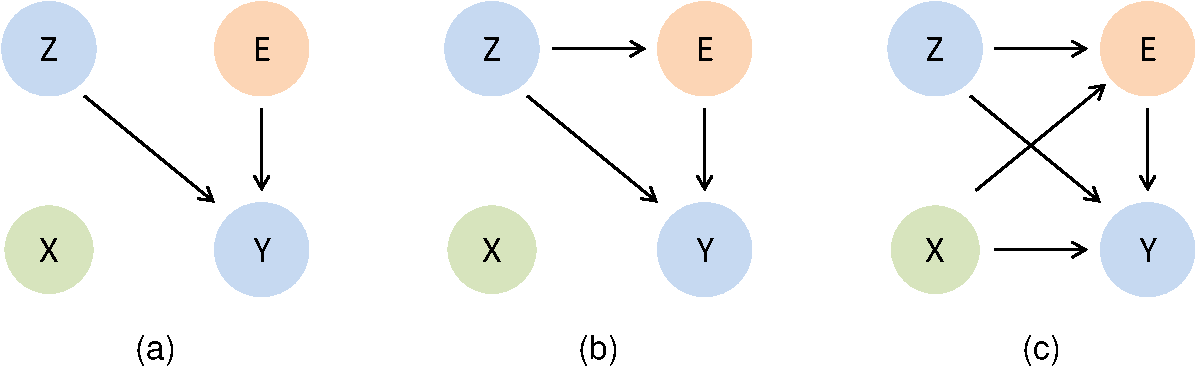
\includegraphics[clip=true, width=0.95\textwidth]{noise-taxonomy.pdf}
    \caption{数据标注噪音类型: (a)完全随机噪音; (b) 随机噪音; (c) 非随机噪音}\label{fig:noise-taxonomy}
\end{figure}

\begin{itemize}
    \item \textbf{完全随机噪音(NCAR)}。噪音$E$独立于其他随机变量,包括真实的标注$Z$。
    \item \textbf{随机噪音(NAR)}。噪音$E$独立于数据$X$, 但依赖真实的标注$Z$。
        该模型允许非对称噪音,即某些类别的数据更有可能出现标注噪音。
        随机噪音可等价地表示为一个标注矩阵或转移矩阵:
        \begin{eqnarray}
            \gamma =
            \begin{pmatrix}
                \gamma_{11} & \cdots & \gamma_{1K} \\
                \vdots & \ddots & \vdots \\
                \gamma_{K1} & \cdots & \gamma_{KK}
            \end{pmatrix}
            =
            \begin{pmatrix}
                \P(Y = 1|Z=1) & \cdots & \P(Y= K|Z=1) \\
                \vdots & \ddots & \vdots \\
                \P(Y = 1|Z=K) & \cdots & \P(Y = K|Z=K)
            \end{pmatrix}
        \end{eqnarray}
    \item \textbf{非随机噪音(NNAR)}。上述两种噪音类型均假设标注噪音对于同一类别下的
        所有样本具有相同的影响。然而在实际场景中,上述假设不一定成立。例如,
        当样本与其他类别样本之间的距离较近时,更有可能发生错误标注。此外,
        样本分布密度较低的区域标注的可靠性也比其它区域低。在图~\ref{fig:noise-taxonomy}(c)所示的
        模型中,标注噪音$E$同时依赖于数据$X$和真实类别$Y$,错误标注更有可能
        出现在某些类别和数据空间的某些区域。非随机噪音是最有普适性
        的噪音类型。例如,分界面附近和低样本密度分布区域的标注噪音只能用非随机噪音
        来建模。
\end{itemize}

\section{弱监督相关反馈深度神经网络}
传统弱监督目标识别算法需要人工设计一系列的特征,如全局特征、局部特征等。这些特征的表征能力直接
影响目标识别的效果,不仅提高了研究人员设计特征的难度,也制约了目标识别效果的
提高。近年来,深度卷积神经网络在目标识别上获得了巨大的成功。
2012年,Alex等人将深度卷积神经网络应用到了百万规模的ImageNet目标识别任务上,
提出了AlexNet网络模型,通过5层卷积层和3层全连接层的网络结构,
从原始的图片像素中提取从浅层到深层的语义特征并做目标识别~\cite{krizhevsky2012imagenet}。
深度学习的优点在于不需要人工设计特征,网络通过反向传播的方式同时
学习特征提取和分类器。然而,经典的深度卷积神经网络对数据标注的准确性有很大的依赖性,
如何利用大规模弱监督社交多媒体数据训练深度卷积神经网络成为了近年来的研究热点之一。

\subsection{经典深度卷积神经网络}
如图~\ref{fig:cnn}所示,经典深度卷积神经网络的前几层通常是卷积层,最后几层为全连接层,
不同的任务可能会采用不同深度的网络。假设训练数据为$X=\{(\x_1, y_1), \ldots,
(\x_N, y_N)\}$, $\x_i \in \R^d$表示第i个数据,$y_i \in [0,K-1]$是第i个数据的标注类别,
$K$是类别数目 $N$是图片总数目。假设网络的层数为$M$,网络参数表示为
$W = \{W^1, \ldots, W^M\}$。数据在第$m$层的特征图(Feature Map)表示为
$Z^m(X) = [\z^m(\x_1), \ldots, \z^m(\x_N)]^T \in \R^{N \times d_m}$。
最后一个全连接层的输出$\z^M(\x_i)$作为Softmax分类器的输入,
得到所有类别上的概率分布$\p(\z^M(\x_i))$。

通常,卷积神经网络的损失函数是Softmax函数的负对数似然函数和权重衰减项(weight decay)之和:
\begin{equation}\label{eqn:cnn-loss}
    \L(W;X,\y) = -\frac{1}{N}\Big[\sum_{i=1}^N {\log p(y_i | \x_i; W)}\Big] + \frac{\beta}{2}\|W\|_F,
\end{equation}
其中,$\beta$是
权重衰减项的系数。假设最后一层为全连接层,上述损失函数相对于最后一层特征图$Z^M$以及参数$W^M$的
梯度为:
\begin{eqnarray}
    Z^M &=& Z^{M-1}W^M \\
    \frac{\partial{\L(W;X,Y)}}{\partial{\z^M(\x_i)}} &=&
    -\frac{1}{N} \Big({\one_{y_i}(\z^M(\x_i)) - \p(\z^M(\x_i))}\Big),\\
    \frac{\partial{\L(W;X,Y)}}{\partial{W^M}} &=&
    (Z^{M-1})^T\frac{\partial{\L(W;X,Y)}}{\partial{\z^M(\x_i)}} \nonumber \\
    &=& -\frac{1}{N}\sum_{i=1}^N {\z^{M-1}(x_i) \Big({\one_{y_i}(\z^M(\x_i))
    - \p(\z^M(\x_i))}\Big)^T}.
\end{eqnarray}
其它层参数的梯度通过方向传播(Back Propagation)得到~\cite{lecun1998gradient}。
从上述公式可以看出,错误的标注会导致参数梯度计算错误,并被反向传播,
使得经典的深度卷积神经网络对于标注噪音十分敏感。

\begin{figure}[t]
    \centering
    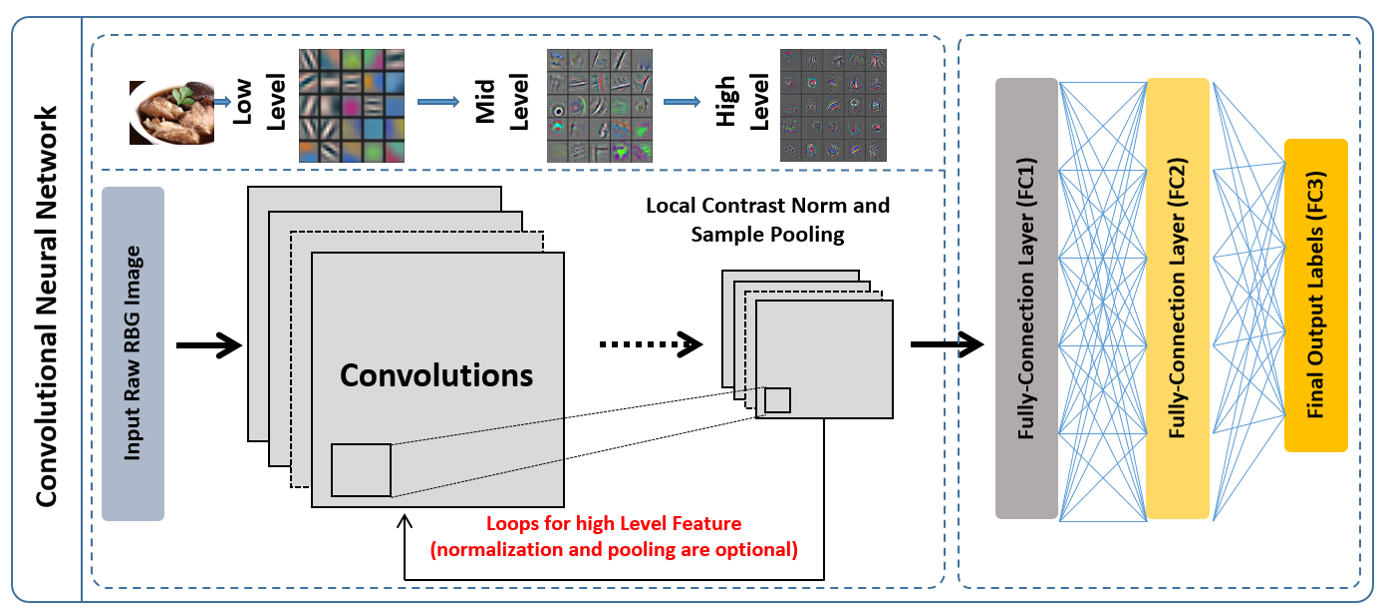
\includegraphics[clip=true, width=0.95\textwidth]{cnn.png}
    \caption{深度卷积神经网络结构图}
    \label{fig:cnn}
\end{figure}

\subsection{相关反馈深度卷积神经网络}
目前已有部分工作研究弱监督深度学习, 然而现有方法大多基于特定的噪音模型,
难以处理真实的场景,或建模过于复杂,难以训练。
2014年谷歌研究团队提出了利用数据特征之间的相似性监督网络学习,
抑制错误标注影响的学习方法~\cite{reed2014training}。文章认为,
如果数据的特征之间具有相似性,那么预测的结果也应该比较相似。
文章将这种关系称之为感知连续性, 并将感知连续性应用到随机噪声假设下的网络学习中。
本章在感知连续性的基础上提出了不依赖于特定噪声类型的相关反馈深度卷积神经网络。

\begin{figure}[t]
    \centering
    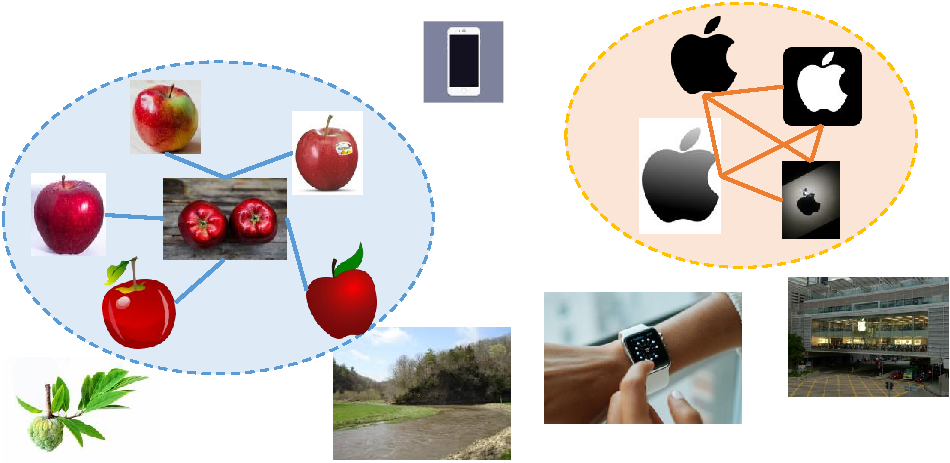
\includegraphics[clip=true, width=0.9\textwidth]{perceptual-consistence.pdf}
    \caption{感知连续性示例}
    \label{fig:perceptual-consistence}
\end{figure}

基于感知连续性,本章提出方法的基本假设是正确标注样本在数据空间具有相似性,
它们的特征在特征空间也具有相似性,而错误标注的样本则不具有这种相似性。
因此,可以利用特征之间的相关性作为反馈,使得不同数据在网络训练过程中发挥不同的作用。
图~\ref{fig:perceptual-consistence}是在搜索引擎中搜索``apple''的部分结果,虚线框中的
数据相互之间比较接近,在训练过程中应该发挥更大的作用,虚线框以外的数据不具有与其他数据
的相似性,为噪音标注的可能性较大,在训练过程中应该发挥较小的作用。

为了表示特征之间的关系,我们将网络最后一层的特征转换为能反映
特征之间相互关系的关联特征表示(Affinity Representation)。类似于
Belkin等人提出的最近邻系统~\cite{belkin2001laplacian},我们定义如下
相似度矩阵$S\in R^{N \times N}$:
\begin{equation}\label{eqn:rf-cnn-sim}
    S_{ij} =
    \begin{cases}
        \exp\{-\frac{\|\z^M(\x_i) - \z^M(\x_j)\|^2}{\gamma^2}\} & y_i = y_j\\
        0 & \text{otherwise},
    \end{cases}
\end{equation}
其中$\gamma$是尺度因子。为了更好地反映相似度矩阵的局部结构,我们用一个对角矩阵$D$
对相似度矩阵进行正则化,$D_{ii} = \sum_{j=1}^N S_{ij}$。
训练数据最终的特征表示为$\Psi(X;W) = [\vpsi(\x_1), \ldots, \vpsi(\x_N)] =
D^{-1}S$,矩阵$\Psi(X;W)$的每一列包含了数据$\x_i$和其他数据特征之间的关系。

假设理想情况下不受噪音影响的模型参数为$W^*$,
噪音鲁棒学习算法应该尽量优化$W$使其逼近$W^*$。
该优化目标可以通过最小化特征表示$\Psi(X;W)$和理想情况下的
特征表示$\Psi(X;W^*)$之间的差值$E_n$得到。$E_n$是由标注噪音引起的特征表示的误差。
换句话说,可以认为$\Psi(X;W)$是理想特征与一个加性噪声之和:
\begin{equation}
    \Psi(X;W) = \Psi(X;W^*) + E_n
    \label{eqn:additive-noise}
\end{equation}
根据方程~\eqref{eqn:additive-noise}以及低秩理论~\cite{candes2011robust},
我们假设$\Psi(X;W^*)$是$\Psi(X;W)$的低秩近似矩阵:
\begin{equation}
    \text{rank}(\Psi(X;W)) > \text{rank}(\Psi(X;W^*))
\end{equation}

在社交多媒体数据上,当类别数目足够多,可以假设错误的标注来自于同一训练数据集上的其他类别,
训练数据的特征最多有$K$个模式,$\Psi(X;W^*)$的秩等于类别数目$K$,因此, $\Psi(X;
W^*)$可以通过如下优化方程得到:
\begin{eqnarray}
    \label{eqn:low-rank}
    \min_{\Psi(X;W^*)} \|\Psi(X;W) - \Psi(X;W^*)\|_F,
    \quad \text{s.t.} \quad  \text{rank}(\Psi(X;W^*)) = K.
\end{eqnarray}

\begin{figure}[t]
    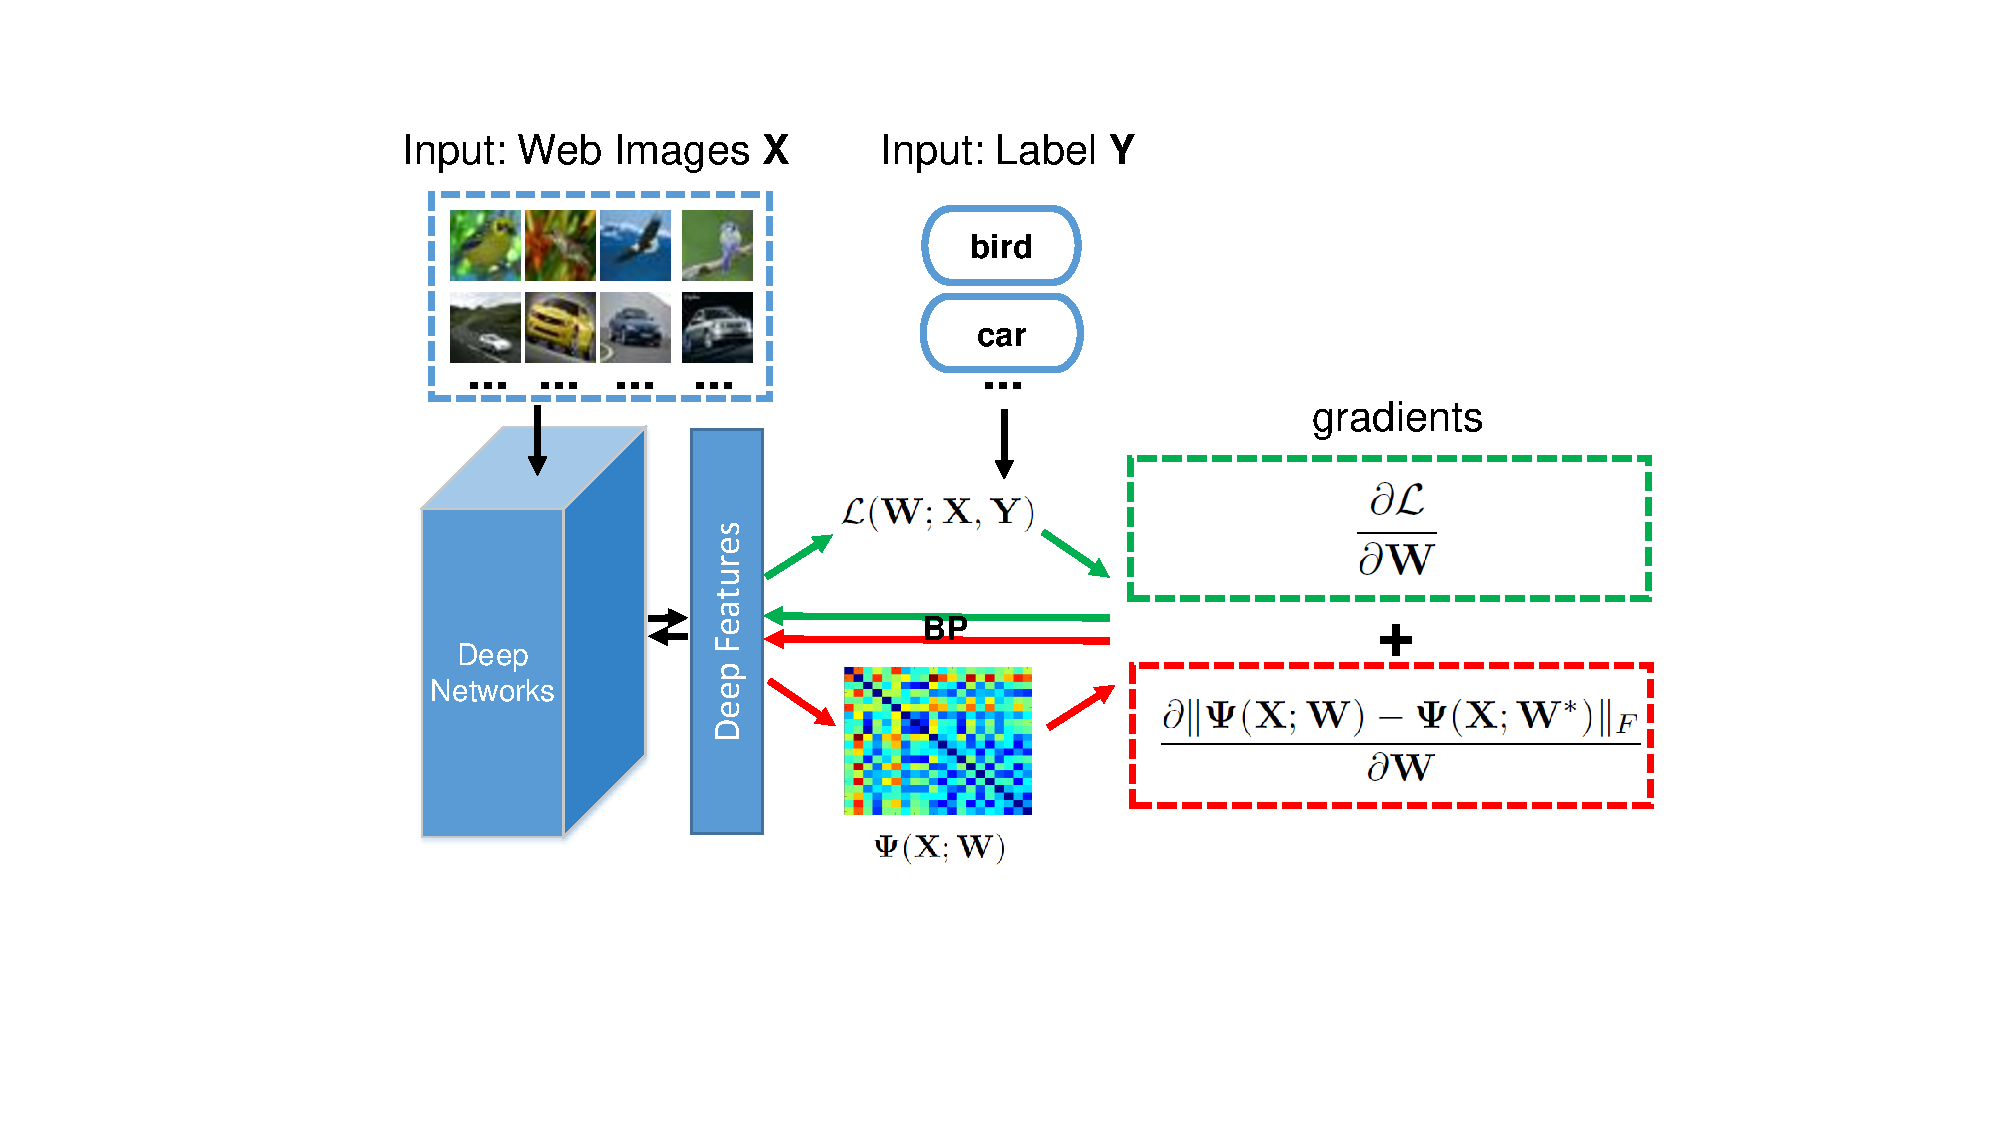
\includegraphics[clip=true, width=0.9\textwidth]{rf-cnn-frm}
    \caption{弱监督相关反馈深度卷积神经网络}\label{fig:rf-cnn-frm}
\end{figure}
如图~\ref{fig:rf-cnn-frm}所示,相关反馈神经网络利用训练数据之间的感知连续性,
通过特征矩阵的重构误差抑制训练过程中噪音的影响。
然而,方程~\eqref{eqn:low-rank}带来的计算量极大增加了优化过程的时间开销。
此外,该方法优化过程分两步:解优化方程~\eqref{eqn:low-rank}和反向传播。
为了解决该方法以上缺点,本章进一步提出了改进的简化和近似算法。改进的算法基于下面的命题:
\begin{proposition}\label{prop:lowrank-spec}
    令$L=D-S, H^* \in R^{N\times K}$由$\Psi(X;W)$的K个最大特征值
    对应的特征向量构成,可以得到:1)方程~\eqref{eqn:low-rank},即$\Psi(X;W)$
    的秩为$K$的最佳近似矩阵由特征向量矩阵$H^*$唯一决定;2)$H^*$也是下列优化方程的最优解:
    \begin{equation}
        \label{eqn:spec-cluster}
        \min_H \text{tr}[H^TLH] \quad \text{s.t.} \quad H^TH = I.
    \end{equation}
    由于方程~\eqref{eqn:low-rank}和方程~\eqref{eqn:spec-cluster}均在$H^*$取得
    最优值,可以认为方程~\eqref{eqn:low-rank}和方程~\eqref{eqn:spec-cluster}
    作为惩罚项是等价的。
\end{proposition}
\begin{proof}
    命题~\ref{prop:lowrank-spec}可以通过如下三个定理得到。
    不失一般性,假设$\text{rank}(\Psi(X;W)) = r$。矩阵的秩为$K$
    的最小重构误差矩阵可以通过\emph{Eckart-Young-Mirsky}
    定理~\cite{eckart1936approximation}得到:
    \begin{theorem}[Eckart-Young-Mirsky]\label{thm:eym}
        对秩为$r$的矩阵$P\in \R^{m\times n}$进行奇异值分解(Singular Value
        Decomposition, SVD)得到$P=U\Sigma V^T, U^TU=I, V^TV=I$,
        如果$K < r$, 则有:
        $$%\begin{equation}
        \argmin_{
            \mbox{\scriptsize
                $
                \begin{array}{c}
                    \hat{P} \in \R^{m\times n} \\
                    \text{rank}(\hat{P}) = K
                \end{array}
                $
            }
        } \|P - \hat{P}\|_F = U\hat{\Sigma}V^T,
        $$%\end{equation}
        其中$\hat{\Sigma}$是包含$P$的前$K$个最大奇异值的对角矩阵。
    \end{theorem}

    此外,如果矩阵$P$是实对称矩阵,它的奇异值和特征值之间具有如下定理所示关系:
    \begin{theorem}\label{thm:evd}
        对实对称矩阵$P$特征值分解得到$P=Q\Lambda Q^T, Q^TQ = I,
        \Lambda = \text{diag}(\lambda_1, \ldots, \lambda_N).
        \lambda_1 \geq \lambda_2 \geq \ldots \geq \lambda_N$是矩阵$P$的特征值。则有
        $$Q=U$$
    \end{theorem}
    因此,根据定理~\ref{thm:eym}和定理~\ref{thm:evd},实对称矩阵$\Psi(X;W)$的秩为$K$
    的最小重构误差矩阵由$\Psi(X;W)$的前$K$个最大特征值对应的特征向量对应的矩阵构成。

    \begin{theorem}[Rayleigh~\cite{golub2012matrix}定理]
        令$H^* = [\h_1^*, \ldots, \h_K^*] = \argmin_{H} \text{tr}[H^TLH]$,
        并且$H^TH = I$,
        则最优解$H^*$可以通过求解如下泛化特征值分解问题得到:
        $$
        L\h_i = (1-\lambda_i) D\h_i,
        $$
        其中$\{1-\lambda_i^* | i = 1,\ldots,
        K\}$是矩阵$\Psi(X;W)$的前K个最大特征值,
        $H^* = \{\h_i^* | i=1, \ldots, K\}$是对应的特征向量。
    \end{theorem}
    由于方程~\eqref{eqn:low-rank}和方程~\eqref{eqn:spec-cluster}均在$H^*$取得
    最优值,可以认为方程~\eqref{eqn:low-rank}和方程~\eqref{eqn:spec-cluster}
    作为惩罚项是等价的。
\end{proof}

通过以上命题和证明可以发现,方程~\eqref{eqn:low-rank}的最优解可以通过
优化方程~\eqref{eqn:spec-cluster}中的最小迹得到。因此,我们提出将最小迹的优化
目标引入到经典的神经网络中,最终的噪音鲁棒深度网络目标方程为:
\begin{equation}\label{eqn:rf-cnn-obj}
    \widetilde{\L} = \L(W;X,Y) + \alpha \text{tr}[H^TLH].
\end{equation}

上述优化方程仍然需要对特征矩阵做特征值分解,本文进一步提出了近似方法。
首先构建标注矩阵$Y = [\y_1,\ldots, \y_N]^T \in \{0,1\}^{N\times K}$, 每一列
$\y_i\in\{0,1\}^{K\times
1}$表示数据$\x_i$的标注向量,并且只有$y_i$位置为非零值。由于$Y$矩阵是在
标注空间上对数据的表述,$H$矩阵是在特征空间上的主成分表述,根据感知连续性,$H$
可以通过如下优化方程近似得到~\cite{yang2011l2,ye2008discriminative}:
\begin{equation}
    \min_{H} \|HH^T - YY^T\|_F^2.
\end{equation}
为了满足$H$矩阵的正交性,一个合理的近似解为$H = Y(Y^TY)^{-\frac{1}{2}}$。

\begin{figure}[t]
    \center
    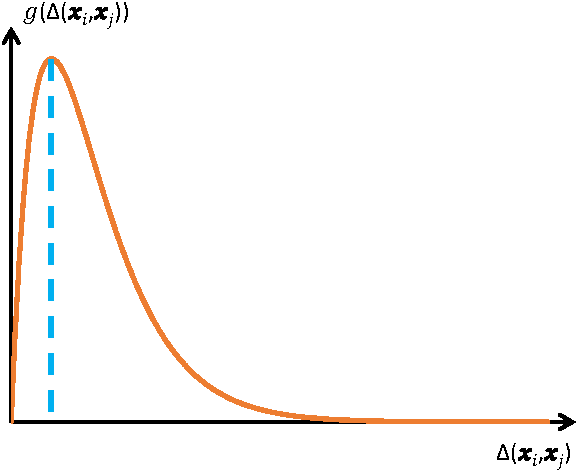
\includegraphics[clip=true, width=0.55\textwidth]{rf-cnn-gradient}
    \caption{训练数据对于梯度的贡献曲线,横坐标为数据与其他数据特征之间的距离}\label{fig:rf-cnn-gradient}
\end{figure}

\subsection{相关反馈分析}
为了验证上述方法有效性,我们从梯度的角度分析相关反馈对于噪声的抑制作用。
定义第$M$层特征之间的距离为:
\begin{eqnarray}
    \Delta(\x_i, \x_j) = \|\z^M(\x_i) - \z^M(\x_j)\|^2
\end{eqnarray}
当$y_i$与$y_j$相同时,$\x_i$和$\x_j$之间的距离$S_{ij}$表示为:
\begin{eqnarray}
    S_{ji}
    = \exp\{-\frac{\|\z^M(\x_j) - \z^M(\x_i)\|^2}{\gamma^2}\}
    = \exp\{-\frac{\Delta(\x_j, \x_i)}{\gamma^2}\}
\end{eqnarray}
$S_{ij}$相对于输入$\z^M(\x_i)$的梯度为:
\begin{eqnarray}
    \frac{\partial S_{ij}}{\partial \z^M(\x_i)} =
    \frac{\partial S_{ij}}{\partial \Delta(\x_i, \x_j)}
    \frac{\partial \Delta(\x_i, \x_j)}{\partial \z^M(\x_i)} =
    \frac{2S_{ij}}{\gamma^2}(\z^M(\x_i) - \z^M(\x_j))
\end{eqnarray}
定义$G=HH^T$,目标方程~\eqref{eqn:rf-cnn-obj}中的相关反馈项对于特征$\z^M(\x_i)$的梯度为:
\begin{eqnarray}
    \frac{\partial tr(H^TLH)}{\partial \z^M(\x_i)} &=&
    \frac{\partial tr(HH^TL)}{\partial \z^M(\x_i)} =
    \frac{\partial tr(GL)}{\partial \z^M(\x_i)}
    =\frac{\sum_{k=1}^N\sum_{j=1}^N{G_{kj}\partial L_{jk}}}{\partial \z^M(\x_i)}
    \nonumber \\
    &=&\frac{\sum_{k=1}^N\sum_{j=1}^N{(G_{kk} - G_{kj})\partial S_{kj}}}{\partial \z^M(\x_i)}
    \nonumber \\
    &=&\frac{2\sum_{k=1}^N\sum_{j=k+1}^N{(G_{kk} - G_{kj})\partial S_{kj}}}{\partial \z^M(\x_i)}
    \nonumber \\
    &=&\sum_{j=i+1}^N{(G_{ii} - G_{ij})}\frac{2\partial S_{ij}}{\partial \z^M(\x_i)}
    \nonumber \\
    &=&\sum_{j=i+1}^N{(G_{ii} - G_{ij})\frac{4S_{ij}}{\gamma^2}(\z^M(\x_i) - \z^M(\x_j))} \\
    \|\frac{\partial tr(H^TLH)}{\partial \z^M(\x_i)}\|^2 &\propto&
    g(\Delta(\x_i, \x_j)) = \Delta(\x_i, \x_j)(\exp\{-\frac{\Delta(\x_i, \x_j)}{\gamma^2}\})^2
\end{eqnarray}

图片$\x_i$对于梯度的贡献是图~\ref{fig:rf-cnn-gradient}所示的单峰函数。
在峰值的右边,随着$\x_i$和$\x_j$之间距离的增大,反馈的梯度逐渐减小至0,意味着
当同一类的样本之间距离过大时,相关反馈的作用较小。在峰值的左边,随着距离减小,
反馈的梯度也减小,距离为0时梯度也为0。这是因为深度学习需要多样化的训练样本,
距离为0意味着两个训练数据完全相同,反馈的梯度也应该为0。

\section{实验结果和评估}
本节从实验的角度验证本章提出的弱监督相关反馈深度神经网络的有效性。
首先在标准数据集上验证该方法对于噪声标注的鲁棒性,其次,我们将该方法用于
真实的社交数据集,验证该方法在社交图片标注上的有效性。

\subsection{目标识别}

\textbf{实验数据}: 我们在两个公开数据集上分别验证算法对噪声的鲁棒性。
一个是Cifar10~\cite{krizhevsky2009learning},
包含$10$个类别$60,000$张$32\times 32$的彩色图片,其中
$50,000$张用于训练,$10,000$张用于测试。 为了产生不同噪声比例的训练数据,
在每个类别的训练数据上按照不同比例,随机选取图片,并将他们的类别随机替换为
数据集中的其他类别,训练数据集的总图片数目保持不变。在我们的实验设置中,
训练数据从无噪声到$90\%$的噪声均匀取$10$个噪声比例。
另一个数据集是PASCAL VOC2007~\cite{pascal-voc-2007},包含$20$个类别总共
$9,963$张图片。我们将数据集随机等分成训练数据和测试数据。

\textbf{比较基准}:本章提出的相关反馈神经网络称为RFCNN,与以下四个方法进行比较:
\begin{itemize}\setlength{\itemsep}{-0.2em}
    \item \textbf{CNN}: 经典的卷积神经网络。
    \item \textbf{RPCA+CNN}: 训练卷积神经网络之前,首先用RPCA~\cite{candes2011robust}
        方法重构训练数据,并移除重构误差较大的数据,移除的比例和噪音的比例相同。
    \item \textbf{CAE+CNN}:用卷积自动编码器预训练卷积神经网络的每一层,
        然后微调整个网络,减小噪音标注的影响~\cite{luo2012hierarchical}。
    \item \textbf{NL+CNN}:用全连接层表示噪音概率矩阵并和卷积神经网络一起训练~\cite{sukhbaatar2014training}。
\end{itemize}
对于VOC2007数据集,我们与另外两种方法进行比较:
\begin{itemize}\setlength{\itemsep}{-0.2em}
    \item \textbf{Best\_VOC}: 在ImageNet数据集预训练网络,
        并在VOC2007上微调~\cite{oquab2014learning}。
    \item \textbf{Web\_HOG}: 在网络图片上基于局部模型和人工设计的特征对图片分类~\cite{divvala2014learning}。
\end{itemize}

\begin{figure}[t]
    \center
    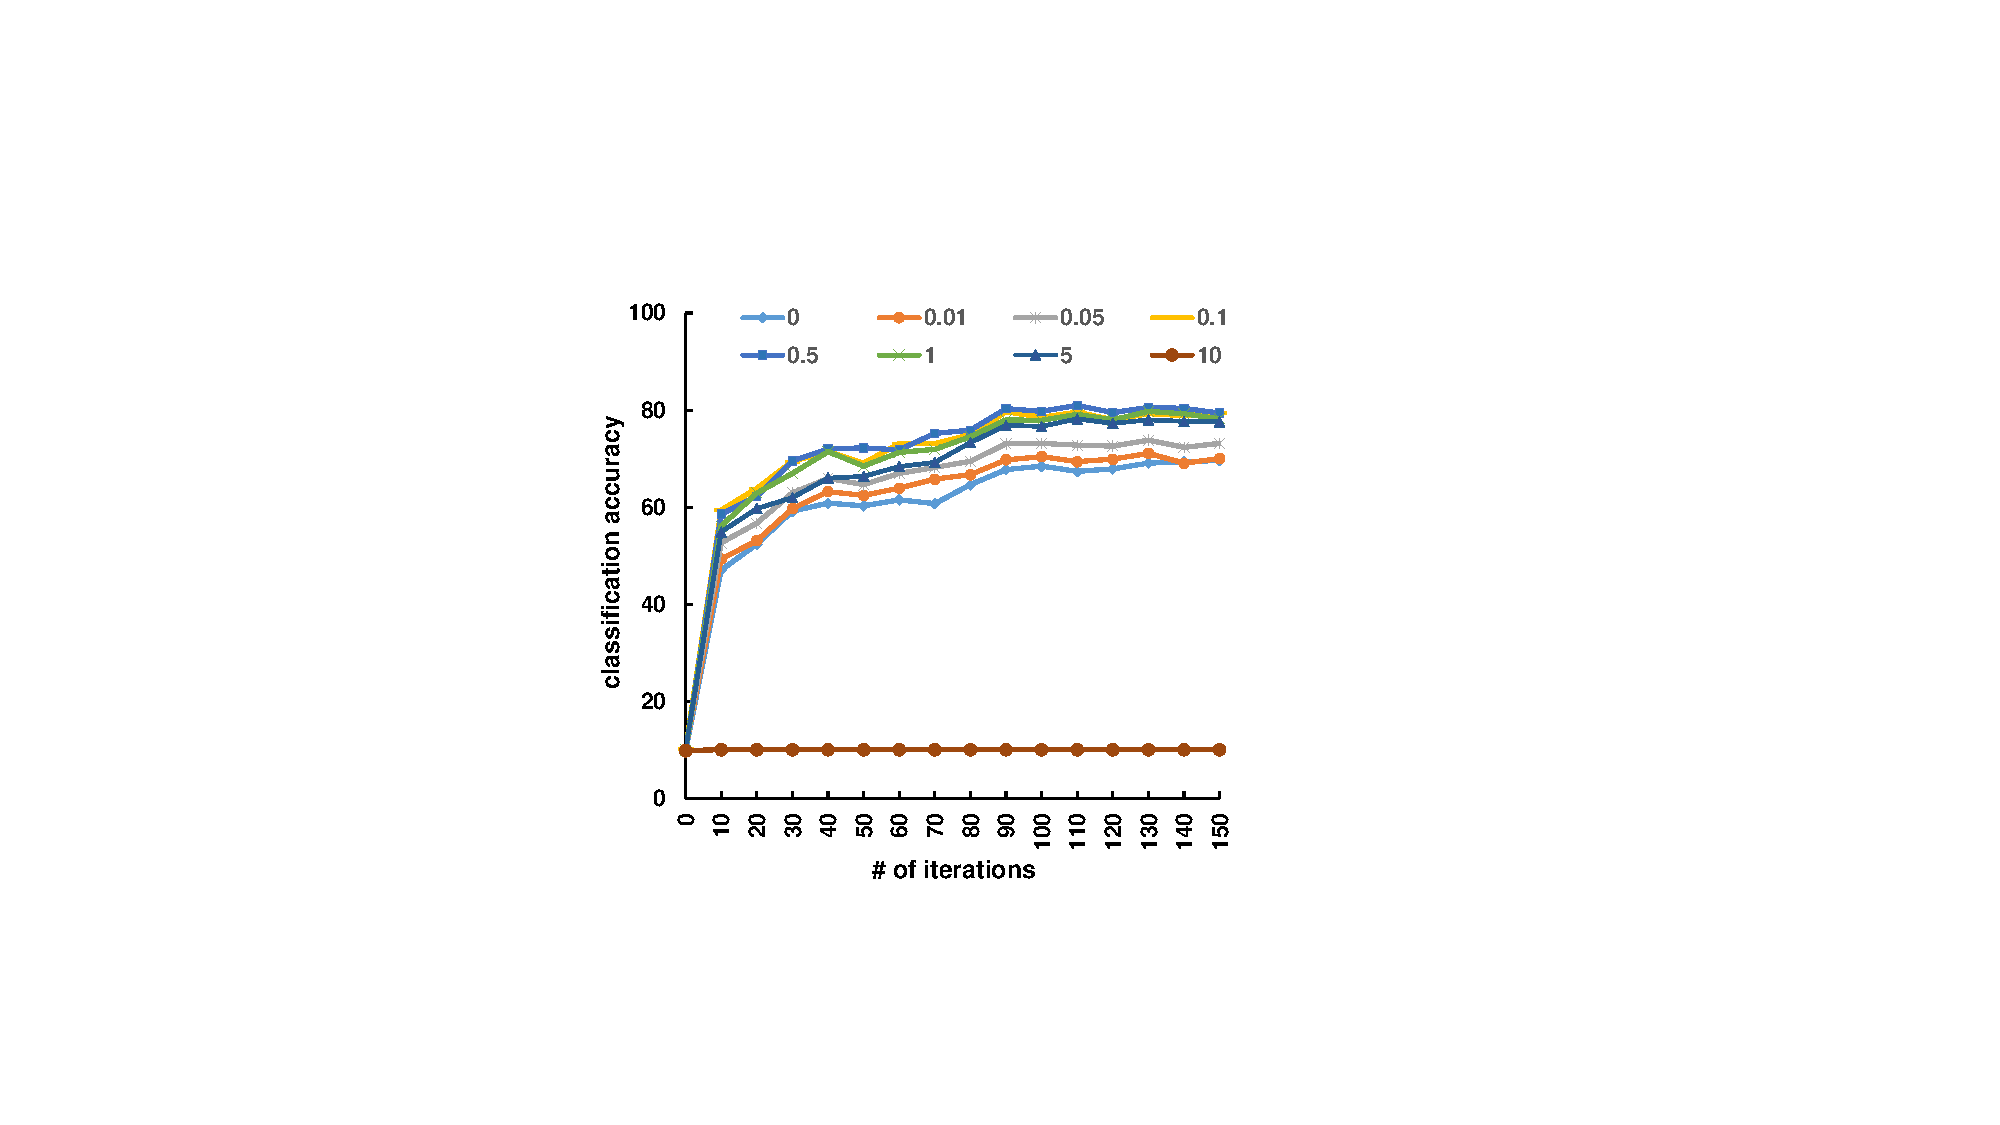
\includegraphics[clip=true, width=0.7\textwidth]{rf-cnn-alpha}
    \caption{参数$\alpha$对于神经网络分类性能的影响}\label{fig:rf-cnn-alpha}
\end{figure}
\textbf{参数设置}:首先,我们调整公式~\eqref{eqn:cnn-loss}
中权重衰减项的系数$\beta$。对于$10\%$的噪音比例,该系数取$0.004$时
网络能达到最好的效果,对于$20\%$的噪音比例,取值为$0.008$,其他噪音比例下取值
为$0.04$。该参数设置对于两个数据集都能取得最好的效果。
此外,我们按照经验将公式~\eqref{eqn:rf-cnn-sim}中的$\gamma$参数设为$0.1$,使得特征相似度在合理的范围。
图~\ref{fig:rf-cnn-alpha}显示了在Cifar10数据集$20\%$噪音下,公式~\eqref{eqn:rf-cnn-obj}中不同$\alpha$取值
对于网络准确率的影响。我们发现,只有当$\alpha$取值过大时(比如取$10$),模型
完全丧失了分类能力,对于其他取值,准确率都保持在相对稳定的范围,并在取值为$0.5$时
达到最优。此外,我们发现$\alpha$取$0.5$在其他噪音条件下也能取得最好的效果。因此,
以下实验$\alpha$均取$0.5$。

\begin{table}[tbp]
    \centering
    \caption{Cifar10数据集上不同算法在不同噪音比例下的准确率比较}
    \label{tab:rf-cnn-cifar10}
    \small
    \tabcolsep=1.5mm
    \begin{tabular}{|c|c|c|c|c|c|c|c|c|c|c|}
        \hline
        \diagbox{\scriptsize{算法}}{\scriptsize{噪声比例}} & 无噪声  & 10\% &  20\% & 30\% & 40\% & 50\% & 60\% & 70\% & 80\% & 90\% \\
        \hline
        CNN & 81.24 & 77.79 & 71.97 & 65.09 & 55.65 & 45.60 & 36.65 & 25.02 & 19.46 & 17.55 \\
        RPCA+CNN & 81.24 & 77.94 & 72.44 & 65.94 & 57.82 & 45.77 & 36.55 & 23.68 & 17.85 & 15.49\\
        CAE+CNN & 81.55 & 78.54 & 73.19 & 67.69 & 60.83 & 52.71 & 44.71 & 34.39 &
        27.54 & 18.61 \\
        NL+CNN & 81.16 & 78.28 & 73.36 & 68.26 & 61.63 & 55.83 & 47.33 & 37.12 &
        30.81 & 19.49 \\
        RFCNN & \textbf{81.60} & \textbf{79.39} & \textbf{76.21} & \textbf{72.81}
        & \textbf{68.79} & \textbf{63.01} & \textbf{54.78} & \textbf{45.48} &
        \textbf{35.43} & \textbf{20.56} \\
        \hline
    \end{tabular}
\end{table}

\begin{figure}[t]
    \vspace{1em}
    \centering
    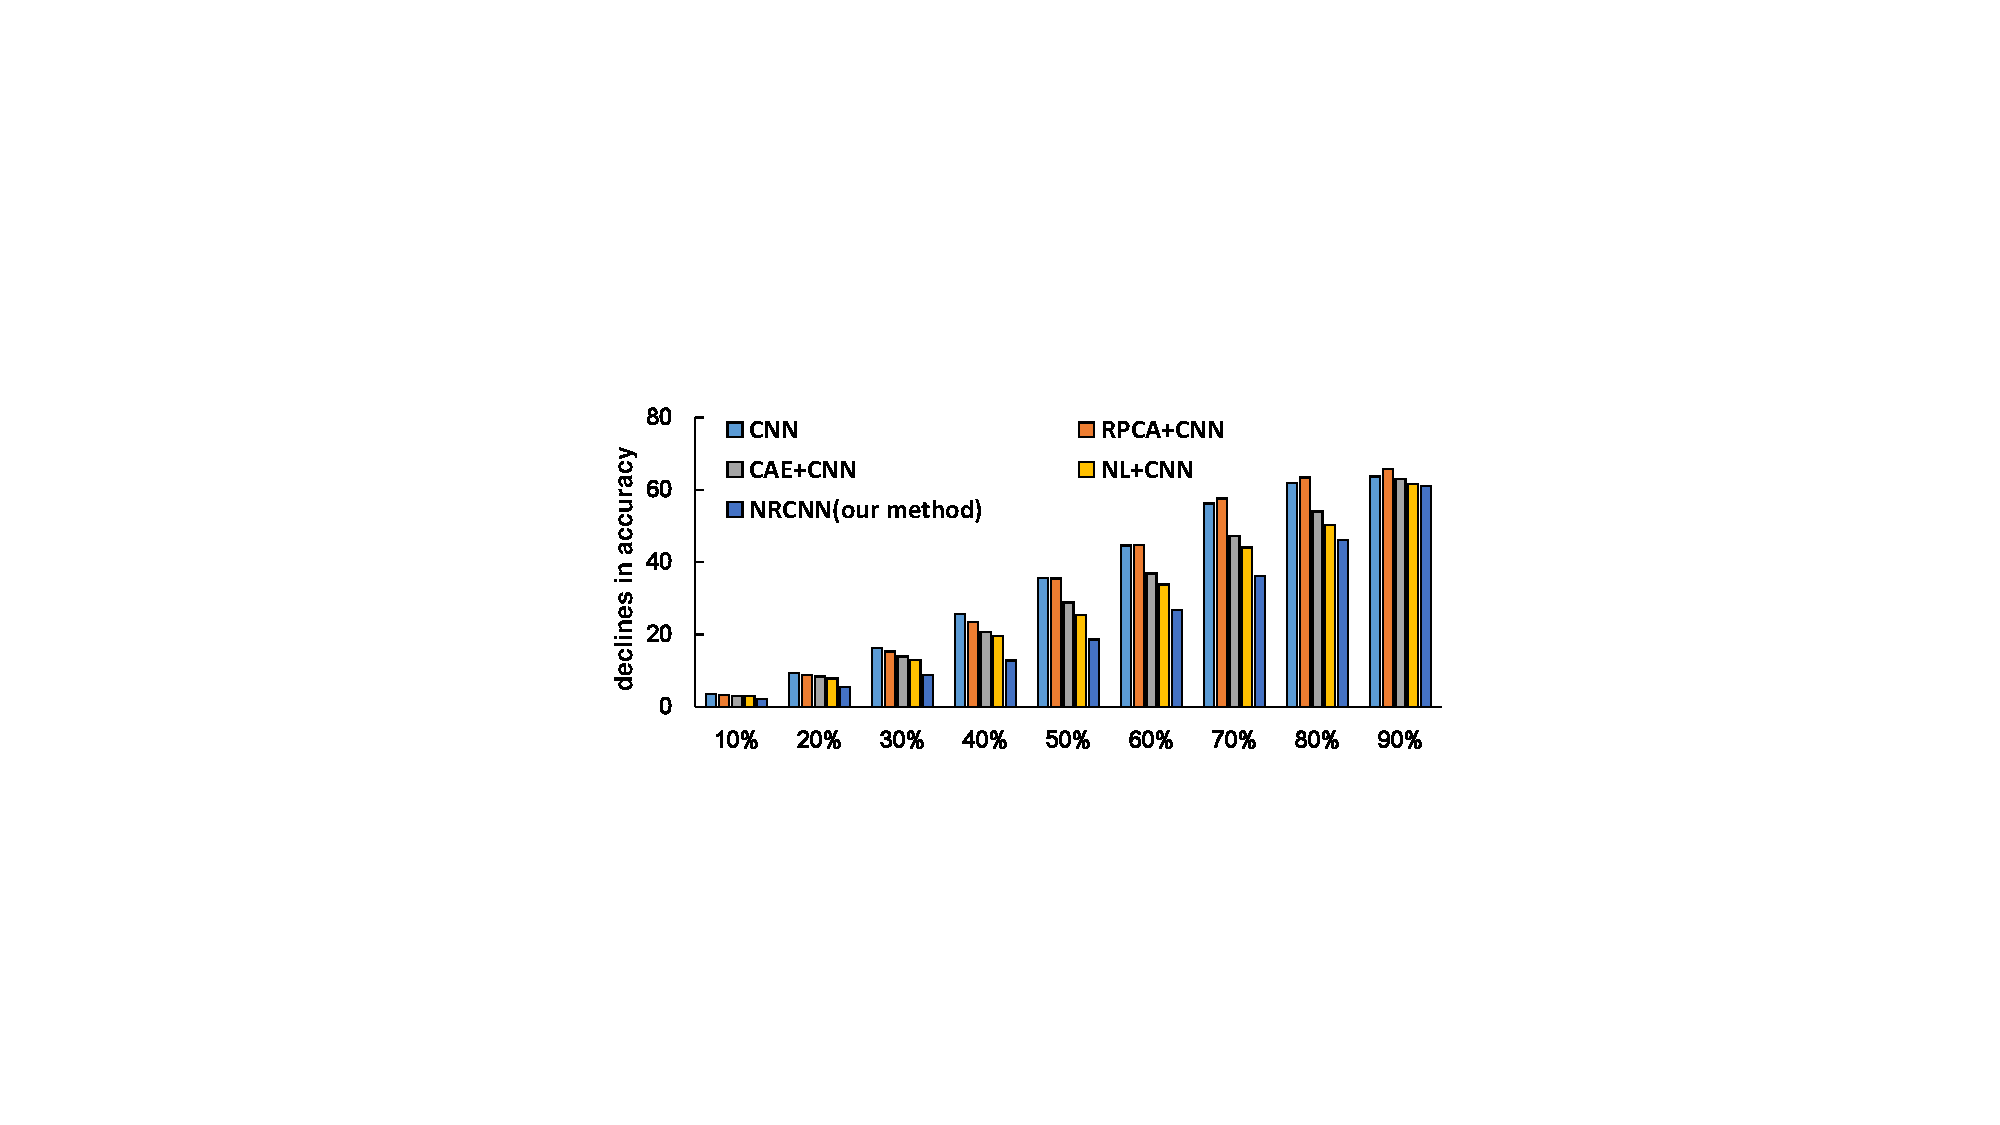
\includegraphics[clip=true, width=0.9\textwidth]{rf-cnn-cifar-decline}
    \caption{不同算法在不同噪音比例下的准确率相对于无噪声准确率的下降程度比较}
    \label{fig:rf-cnn-cifar-decline}
\end{figure}
\textbf{实验结果}:表格~\ref{tab:rf-cnn-cifar10}显示了在Cifar10数据集上不同噪音
程度下不同算法的分类准确率比较。
图~\ref{fig:rf-cnn-cifar-decline}反映了在不同噪音程度下不同方法分类准确率相对于
无噪声下降程度的比较。
本文提出的算法在所有条件下都达到了最好的实验结果,
甚至在无噪声数据集上,我们的算法也比经典的卷积神经网络取得了略好的准确率。我们发现,
在$30\%$数据噪音下,经典卷积神经网络的准确率下降了将近$20\%$,相比之下,本章提出的算法
仅下降了$10\%$,表现出对数据噪音很强的鲁棒性。此外,我们发现数据预处理方法RPCA+CNN在
噪音比例小于$50\%$时,准确率要高于经典的卷积神经网络,当有更多的噪音数据时,
RPCA+CNN的效果则比经典CNN要差。这个现象的原因在于当噪音数据增多时,
数据预处理移除正确数据的风险也随之增大,导致在最终的训练数据中噪音数据的比例增加。
CAE+CNN和NL+CNN算法的性能十分接近,在$30\%$噪音比例下,准确率分别下降$17.0\%$和
$15.9\%$。CAE+CNN虽然能够解决区域级的噪声(背景噪声),但对于样本集噪声(如标注错误),
算法的鲁棒性比较有限。对于NL+CNN,实验证明仅仅在网络上增加一层
噪音适应层并不能达到很好的噪音鲁棒性。相反,本章所提算法可以抑制噪音在所有层的影响。

在PASCAL VOC2007数据集上,我们首先在ImageNet数据集上预训练AlexNet网络~\cite{krizhevsky2012imagenet},然后在网络数据上微调网络参数。为了获取网络数据,
我们将数据集的每个类别作为查询词抓取搜索引擎的返回结果,并滤除重复的图片。
我们收集了两个训练数据集,第一个数据集中正负样本的数目和VOC2007中相同,
在该数据集上的实验我们记为CNN(Web)和RFCNN(Web)。第二个数据集中我们将正样本的
数目增加到VOC2007的4倍,并将该数据集上的方法记为CNN(Webx4)和RFCNN(Webx4)。
根据统计的结果,两个数据集上的噪音比例分别是$20\%$和$40\%$。不同方法
在VOC2007测试数据集上的平均准确率如表~\ref{tab:rf-cnn-voc2007}所示。
可以发现:
\begin{itemize}\setlength{\itemsep}{-0.2em}
    \item CNN(Web)相比Web\_HOG具有十分明显的提升,证明了深度学习网络比基于人工设计的特征
        训练的分类模型具有更强的噪声鲁棒性。
    \item 相比于在有限的标注好的数据集上训练深度模型,RFCNN(Webx4)取得了更好的效果。
\end{itemize}

\begin{table}[tbp]
    \centering
    \caption{VOC2007数据集上不同算法在不同噪音比例下不同类别的平均准确率比较}
    \label{tab:rf-cnn-voc2007}
    \small
    \begin{tabular}{|c|c|c|c|c|c|c|}
        \hline
        \multirow{2}{*}{\diagbox{\scriptsize{类别}}{\scriptsize{算法}}} &
        \multirow{2}{*}{Best\_VOC} & \multirow{2}{*}{Web\_HOG} &
        CNN & CNN & RFCNN & RFCNN \\ 
        &  & & (Web) & (Webx4) & (Web) & (Webx4)
        \\ \hline
        Aeroplanes & 88.5 & 68.5 & 84.1 & 85.4 & 85.8 & \textbf{91.3}
        \\ \hline
        Bicycles & \textbf{81.5} & 48.2 & 68.8 & 69.4 & 69.7 & 75.2
        \\ \hline
        Birds & \textbf{87.9} & 47.3 & 77.1 & 77.1 & 77.4 & 83.3
        \\ \hline
        Boats & \textbf{82.0} & 55.7 & 73.0 & 74.5 & 75.1 & 81.5
        \\ \hline
        Bottles & 47.5 & 40.0 & 63.0 & 63.7 & 63.8 & \textbf{70.2}
        \\ \hline
        Buses &  75.5 & 56.3 & 74.2 & 74.7 & 75.8 & \textbf{81.3}
        \\ \hline
        Cars & \textbf{90.1} & 60.1 & 74.3 & 75.0 & 75.6 & 80.6
        \\ \hline
        Cats & 87.2 & 64.1 & 79.2 & 81.6 & 82.7 & \textbf{88.3}
        \\ \hline
        Chairs & 61.6 & 43.6 & 61.8 & 62.3 & 62.7 & \textbf{67.0}
        \\ \hline
        Cows & 75.7 & 59.2 & 73.8 & 75.7 & 76.9 & \textbf{82.5}
        \\ \hline
        Dining tables & \textbf{67.3} & 32.9 & 48.9 & 53.3 & 53.5 & 60.0
        \\ \hline
        Dogs & 85.5 & 46.5 & 79.5 & 80.2 & 80.6 & \textbf{86.3}
        \\ \hline
        Horses & 83.5 & 56.2 & 81.0& 83.8 & 84.7 & \textbf{90.0}
        \\ \hline
        Motorbikes & 80.0 & 62.4 & 82.1 & 84.6 & 84.9 & \textbf{90.3}
        \\ \hline
        People & \textbf{95.6} & 41.3 & 48.4 & 50.7 & 49.2 & 75.8
        \\ \hline
        Potted plants & 60.8 & 29.6 & 57.9 & 58.9 & 59.1 & \textbf{64.8}
        \\ \hline
        Sheep & 76.8 & 41.4 & 72.0 & 75.9 & 76.0 & \textbf{81.0}
        \\ \hline
        Sofas & \textbf{58.0} & 35.6 & 31.6 & 41.0 & 50.8 & 57.8
        \\ \hline
        Trains & \textbf{90.4} & 68.9 & 83.4 & 84.5 & 84.8 & 89.9
        \\ \hline
        TV/Monitors & \textbf{77.9} & 35.5 & 64.7 & 69.1 & 69.2 & 74.9
        \\ \hline
        \textbf{mAP} & 77.7 & 49.6 & 68.9 & 71.1 & 71.9 & \textbf{78.6}
        \\ \hline
    \end{tabular}
\end{table}

\subsection{社交图片标注}
本章提出的弱监督相关反馈深度卷积神经网络可以大量的社交图片作为训练数据,
可以用于任意类别的社交图片标注。例如,社交图片中广泛存在的``风景'',``家庭''等标签并没有
相应的标注好的训练数据。

\begin{table}[tbp]
    \centering
    \caption{社交图片标注结果比较} \label{tab:rl-social-tagging-comp}
    \footnotesize
    \tabcolsep=0.3mm
    \begin{tabular}{|c|c|c|c|c|c|c|c|}
        \hline
        & CNN(Web) & RPCA+CNN(Web) & CAE+CNN(Web) & NL+CNN(Web) & CNN(ImageNet) &
        DeViSE & RFCNN\\
        \hline
        NDCG@1 & 0.08 & 0.23 & 0.11 & 0.24 & 0.20 & 0.28 & \textbf{0.32}\\
        \hline
        NDCG@3 & 0.18 & 0.32 & 0.25 & 0.33 & 0.29 & 0.36 & \textbf{0.41}\\
        \hline
        NDCG@5 & 0.26 & 0.39 & 0.34 & 0.41 & 0.39 & 0.43 & \textbf{0.46}\\
        \hline
    \end{tabular}
\end{table}

\begin{figure}[t]
    \center
    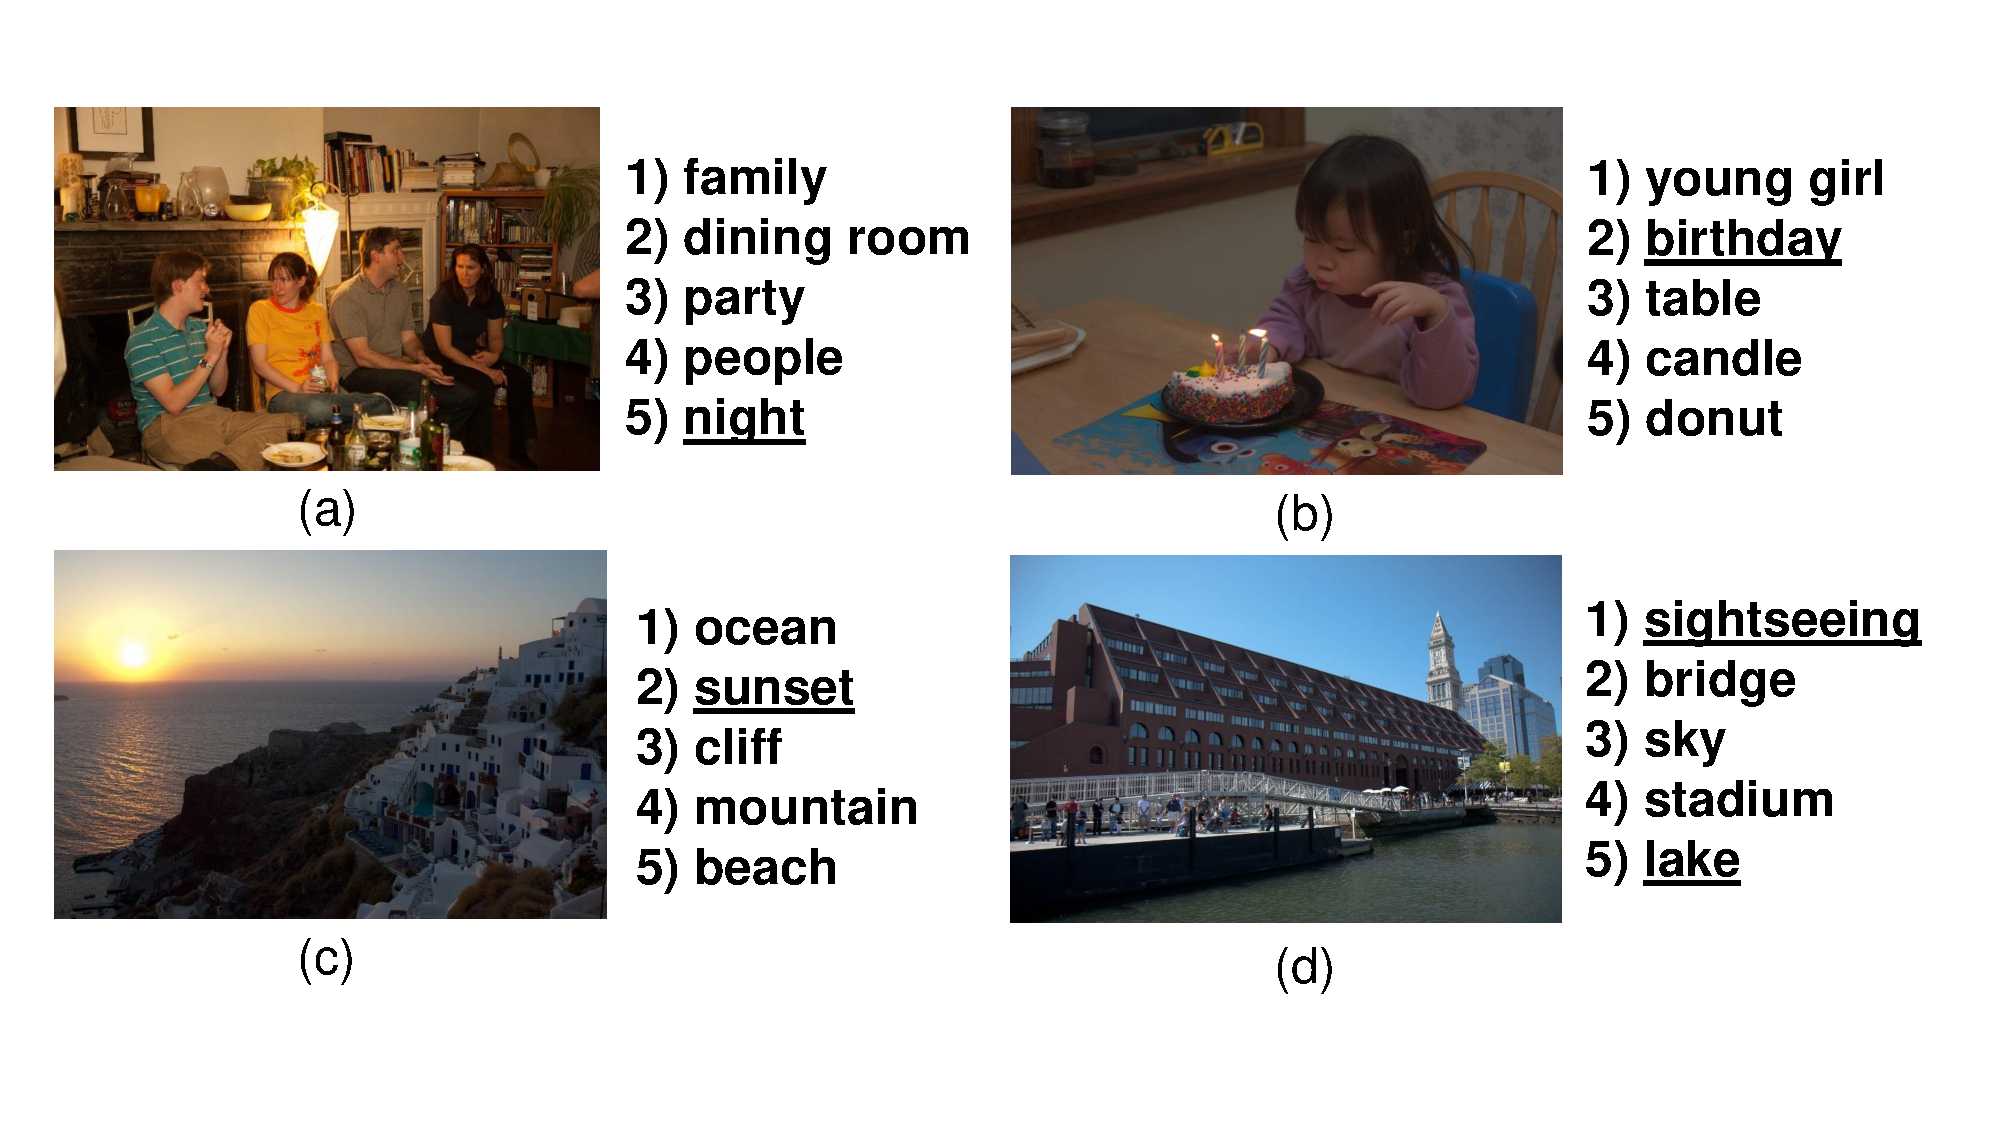
\includegraphics[clip=true, width=0.9\textwidth]{rf-cnn-tagging}
    \caption{社交图片标注结果示例}
    \label{fig:rf-cnn-tagging}
\end{figure}
我们根据Flickr\footnote{\url{https://www.flickr.com/}}上$100,000$名活跃用户(注册
超过2年并在过去6个月上传超过500张照片)提供的标签中选取了200个常见标签,
其中50个标签例如``日落'',``观光'',``生日''等没有在ImageNet数据集中出现。实验中的基准方法采用了ImageNet数据集。
对于这200个标签,我们仅用ImageNet数据集提供的每类$1,000$张图片作为训练数据训练模型,该方法称为\textbf{CNN(ImageNet)}。
此外,我们还采用了视觉语义嵌套方法DeViSE~\cite{frome2013devise},在150个已有训练数据类别上
训练视觉语义嵌套模型,对200个类别进行标注。
对于我们的方法,为了获得完整的200个类别的数据,我们从搜索引擎上为每个类别抓取$1,000$张图片,
移除重复图片并训练模型。网络模型与VOC2007实验中相同。

为了测试不同算法的性能,我们从\textbf{MIT-Adobe FiveK}数据集~\cite{fivek}中随机选取了
$1,000$张图片作为测试集。每种方法根据预测的分数为每张图生成5个有序标签。我们邀请了25位
标注人员为每个标签打分:2—非常相关;1—相关;0—不相关。我们采用归一化折扣增益值(Normalized
Discounted Cumulative Gain,NDCG)作为评价指标。NDCG可以评价不同级别的相关性,相关结果越靠前得到的评分越高。有序结果中
位置$p$的NDCG定义为:
\begin{eqnarray}
    \text{NDCG}@p = Z_p \sum_{i=1}^p \frac{2^{r^i} - 1}{\log{(1+i)}}
\end{eqnarray}
其中$2^{r^i}$是第$i$个标签的相关性评价,$Z_p$是归一化参数。

表格~\ref{tab:rl-social-tagging-comp}显示了相关性评价结果。相比于其它噪音鲁棒算法,
本章提出的方法获得了最好的效果。此外,CNN(ImageNet)数据集由于训练的标注空间较小,
效果较差,证明了利用社交图片的有效性。
本章算法的效果也比视觉语义嵌套方法DeViSE要好。

图~\ref{fig:rf-cnn-tagging}显示了本章提出的弱监督相关反馈深度卷积神经网络在社交图片
上标注结果的示例,其中有下划线的标注没有在ImageNet数据集中出现。

\section{本章小结}
本章提出了弱监督相关反馈深度卷积神经网络,从大量的弱标注社交多媒体数据中学习目标识别模型。
算法利用了训练数据之间的相关性使得不同的训练数据在网络训练中有不同的梯度贡献,抑制
了训练数据中标注噪音的影响,实现了在不需要人工标注的情况下快速学习任意的语义类别。
为了提高算法的效率,本章对弱监督相关反馈深度神经网络做了进一步的简化和近似。
本章在混入噪音的标准数据集和真实的社交图片上进行了实验,验证了算法的对于标注噪音
的鲁棒性。

本章的主要贡献包括:
\vspace{-0.5em}
\begin{itemize}\setlength{\itemsep}{-0.2em}
    \item 基于感知连续性提出了端到端的弱监督相关反馈神经网络,
        直接从弱标注社交多媒体数据中学习任意语义类别。
    \item 对相关反馈网络做了简化近似,提高了算法的计算速度。
    \item 本章提出的弱监督相关反馈深度神经网络不依赖特定的网络结构,可以方便地
        应用到更复杂的网络结构和应用场景。
\end{itemize}

\chapter{大规模社交多媒体数据快速处理}
社交多媒体数据由于规模庞大,需要耗费大量的计算资源和处理时间。本章从特征选取
和模型简化两个角度讨论大规模社交多媒体数据的快速处理。

本章首先介绍用于大规模高维数据的特征选取算法。 社交多媒体数据的特征包括深度网络特征、全局特征、
局部特征等,实际应用中需要根据特定的需求选取对目标任务最有用的特征,
这对于提高大规模社交多媒体数据的处理速度
以及在计算能力、内存空间和电池续航都十分有限的移动设备上处理社交多媒体数据都具有重要意义。
此外,去除与特定任务不相干的特征,还可以提高特征的表达能力。

其次,本章介绍用于深度卷积神经网络的模型简化算法。
深度卷积神经网络在很多计算机视觉领域都表现出很好的效果,
然而大量的模型参数需要大量的计算资源和时间,极大地限制了深度卷积神经网络
在实际场景中的应用。此外,深度网络在移动设备上的应用已经成为一种趋势,
由于移动设备计算能力的限制,在不影响模型准确率的条件下简化深度网络模型已经成为迫
切的需要。

\section{在线特征选取问题建模}
特征选取是指从数据中移除不相关或冗余的特征。在当前大数据的背景下,特征选取
已经成为了十分重要的技术,并在多个领域尤其是大规模高维数据的场景下获得了
广泛应用~\cite{Bolon015RAE,Zhai14EBD}。尽管特征选取已经被广泛地研究,大部分的算法
都属于批处理学习。批处理学习的主要问题在于需要将整个数据集加载到内存中,
对于实际问题中的大规模高维数据不具有可伸缩性。此外,
批处理方法假设所有的训练数据和特征在训练前已经确定,
而实际场景中需要处理的通常是流数据,并可能伴随有新的特征出现。
为了克服批处理算法的这些问题,近年来有部分工作研究在线特征选取~\cite{wang2014online,wu2010online,yang2013efficient}。
在线学习的优点在于算法每次迭代只处理一个数据,因此具有很高的伸缩性,
并且可以很好地应对数据中模式和特征的变化。然而,目前已有的在线特征选取算法复杂度仍然过高,
算法的准确率与批处理方法也有不小差距。
因此,本章提出了快速二阶在线特征选取算法,
不仅对于大规模高维数据具有很高的可伸缩性和学习效率,
算法的准确率也与批处理方法十分接近。

不失一般性,本章首先研究二分类问题,并在~\ref{ssec:smofs}节将算法扩展到多类问题。
令$\{(\x^t,y^t)|t=1,\ldots, T\}$表示训练过程中依次收到的数据,每个数据$\x^t
\in \R^d$是一个$d$维的向量,数据类别$y^t\in\{+1,-1\}$。
在线学习算法学习一个相同维度的线性分类器$\w \in \R^d$。
在时刻$t$,算法接收到数据$\x^t$,基于当前的模型参数$\w^t$预测它的类别$\hat{y}\in\{+1,-1\}$。
\begin{equation}\label{eqn:predict}
    \hat{y}^t = \sign(\w^t \cdot \x^t).
\end{equation}
预测以后,算法得到真实的类别$y^t$,并衡量在数据$(\x^t,y^t)$上的损失函数$\ell(\w^t)$。
损失函数通常为真实类别和预测结果的函数。根据损失函数和特定的更新规则,算法更新
模型参数$\w^t$。例如,在线梯度下降算法更新的规则为:
\begin{equation}
    \w^{t+1} = \w^t + \eta^ty^t\x^t,
\end{equation}
$\eta^t$是时刻$t$的学习率(Learning Rate)。根据不同的更新规则,在线学习算法可以分为两类:
\vspace{-0.8em}
\begin{itemize}\setlength{\itemsep}{-0.5em}
    \item 一阶算法:本质上是梯度下降算法~\cite{crammer2006online};
    \item 二阶算法:挖掘输入数据几何特点~\cite{crammer2009adaptive}
        或构建目标方程的近似海森矩阵~\cite{duchi2011adaptive};
\end{itemize}

在线特征选取算法对$\w$的$L_0$范式施加公式~\eqref{equ:sofs-l0-norm}中所示约束,
选取权重向量$\w^t$中相对较少的一部分元素,并将其他元素设为$0$。
\begin{equation}
    \label{equ:sofs-l0-norm}
    \|\w\|_0 \leq B, \|\w\|_0 = \sum_{i=1}^d w_i^0,
\end{equation}
其中$B$是预先定义的常数。相应地,只有与$\w$中非零权重对应的$\x$的$B$个特征被选取。

\section{置信度加权二阶在线特征选取}
在线特征选取最直接的算法是截断感知机算法(Perceptron with Truncation, PET)~\cite{wang2014online}。
具体来说,分类器在每次迭代时首先根据$\w^t$预测类别$\hat{y}^t$并计算损失函数$\ell(\w^t)$。
如果$\ell(\w^t)$大于0,则$\w^{t+1}=\w^t$;
否则,分类器根据感知机规则更新$\w^{t+1}$:$\hat{\w}^{t+1} = \w^t + \eta y^t\x^t$。
算法保留更新后参数绝对值最大的$B$个元素,其他元素设为$0$。截断后的分类器参数
$\w^{t+1}$被用于下一轮迭代的预测和更新。算法~\ref{alg:pet}显示了PET算法的框架,
算法~\ref{alg:truncate}显示了在线特征选取的截断函数。

\begin{algorithm}[t]
    \SetKwData{Left}{left}\SetKwData{This}{this}\SetKwData{Up}{up}
    \SetKwFunction{Union}{Union}\SetKwFunction{FindCompress}{FindCompress}
    \SetKwInOut{Input}{input}\SetKwInOut{Output}{output}

    \Input{$B$ - 需要选取的特征个数,$\eta$ - 学习率}
    \Output{权重向量$\w^T$}
    \BlankLine
    初始化$\w^1 = \zero$\;
    \For{$i\leftarrow 1$ \KwTo $T$}{
        接收到数据$\x^t\in \R^d$,预测类别$\hat{y}^t = \sign(\w^t\cdot \x^t)$\;
        接收真实类别$y^t$\;
        计算损失函数$\ell(\w^t)$\;
        \If{$\ell(\w^t)>0$}{
            $\hat{\w}^{t+1} = \w^t + \eta y^t \x^t$\;
            $\w^{t+1} = \Truncate(\hat{\w}^{t+1},B)$\;
        }
    }
    \caption{PET——截断感知机算法}\label{alg:pet}
\end{algorithm}

\begin{algorithm}[t]
    \SetKwData{Left}{left}\SetKwData{This}{this}\SetKwData{Up}{up}
    \SetKwFunction{Union}{Union}\SetKwFunction{FindCompress}{FindCompress}
    \SetKwInOut{Input}{input}\SetKwInOut{Output}{output}

    \Input{$\hat{\w}$ - 权重向量,$B$ - 需要选取的特征个数}
    \Output{截断的权重向量$\w$}
    \BlankLine
    $\w=\hat{\w}$\;
    \If{$\|\hat{\w}\|_0 > B$}{
        除了$\w$的绝对值最大的$B$个元素,其他元素全部设为0\;
    }
    \caption{Truncate——截断函数}\label{alg:truncate}
\end{algorithm}

根据Wang等人的分析,上述算法在实际应用中并不总能取得很好的效果~\cite{wang2014online}。
它不能保证被截断的参数足够小,因而不能保证很小的错误率。
因此,Wang等人提出了一阶在线特征选区(First Order Feature Selection, FOFS)算法,
在截断之前对权重向量做稀疏投影。FOFS算法保证了每次迭代时分类器参数$\w^t$都限制在一个$L_1$范式
约束的超体内部。算法~\ref{alg:fofs}显示了FOFS算法的细节。

\begin{algorithm}
    \SetKwData{Left}{left}\SetKwData{This}{this}\SetKwData{Up}{up}
    \SetKwFunction{Union}{Union}\SetKwFunction{FindCompress}{FindCompress}
    \SetKwInOut{Input}{input}\SetKwInOut{Output}{output}

    \Input{$B$ - 需要选取的特征个数,$\eta$ - 学习率,$\lambda$ - 正则化参数}
    \Output{截断的权重向量$\w$}
    \BlankLine
    $\tilde{\w}^{t+1} = (1-\lambda\eta)\w^t + \eta y^t \x^t$\;
    $\hat{\w}^{t+1} = \min\{1,\frac{\frac{1}{\sqrt{\lambda}}}{\|\tilde{\w}^{t+1}\|_2}\tilde{\w}^{t+1}\}$\;
    $\w^{t+1} = \Truncate(\hat{\w}^{t+1}, B)$\;
    \caption{FOFS——一阶在线特征选取算法}\label{alg:fofs}
\end{algorithm}

一般来说,一阶在线特征选取算法的复杂度和特征维度成正比。对于超高维度数据,
算法的速度比较慢。此外,当输入数据的不同维度特征不在同一个尺度时,一阶算法
可能会移除有价值的特征。如公式~\eqref{eqn:predict}所示,预测结果不仅依赖于
权重向量,也依赖于输入数据。即使$|w_i|<|w_j|$,
也不能保证$|w_i * E(x_i)| < |w_j * E(x_j)|$,$E(x_i)$是$x_i$的期望。为了克服
一阶算法的局限性,我们探索了二阶在线学习的最新发展,
提出了置信度加权二阶在线特征选取(Second Order Feature Selection, SOFS)算法。

置信度加权二阶在线学习算法~\cite{dredze2008confidence}假设线性分类器的权重向量服从高斯分布
$\w\sim \Nn(\Mu, \Sigma)$。权重的置信度通过协方差矩阵$\Sigma$的对角元素表示,
对角元素$\Sigma_{jj}$越小,权重$w_j$的均值的置信度越高。算法在接收到训练数据之前,
所有权重有共同的置信度或不确定性。训练过程中,给定一个接收到的
训练数据$(\x^t,y^t)$,置信度加权算法更新权重使得在当前数据$\x^t$上做出正确预测的
概率大于一个阈值$\tau$。同时,算法尽量保持与更新前的权重分布相同。置信度加权算法
可以表示为如下所示优化问题:
\begin{eqnarray} \label{eqn:prob}
    (\hat{\Mu}^{t+1},\Sigma^{t+1}) &=&
    \argmin_{\Mu,\Sigma}{\DKL(\Nn(\Mu,\Sigma), \Nn(\Mu^t,\Sigma^t))}
    \nonumber \\
    s.t. &&\Pr_{\w\sim\Nn(\Mu,\Sigma)}[y^t(\w\cdot \x^t) \geq 0]  \geq \tau,
\end{eqnarray}
其中$\DKL(*,*)$是Kullback-Leibler(KL)距离。两个高斯分布$\Nn(\Mu,\Sigma)$和
$\Nn(\Mu^t,\Sigma^t)$的KL距离定义为:
\begin{eqnarray}
    \DKL(\Nn(\Mu,\Sigma), \Nn(\Mu^t,\Sigma^t)) &=&
    \frac{1}{2}\log{\frac{\text{det}\Sigma^t}{\text{det}\Sigma}}
    + \frac{1}{2}\text{Tr}((\Sigma^t)^{-1}\Sigma) \nonumber \\
    &+& \frac{1}{2}(\Mu^t - \Mu)^T(\Sigma^t)^{-1}(\Mu^t - \Mu) - \frac{d}{2}.
\end{eqnarray}
公式\eqref{eqn:prob}中的约束可以重新表达为:
$y^t(\Mu\cdot \x^t)  \geq  \phi\sqrt{(\x^t)^T\Sigma\x^t}$,
$\phi = \Phi^{-1}(\tau)$ ($\Phi$是高斯分布的累积函数)。
研究人员提出了多种方法解公式~\eqref{eqn:prob}中的优化问题。本章
采用能够对每个训练数据的预测函数进行自适应正则化的AROW算法~\cite{crammer2009adaptive}。
研究和实验表明,该算法对于训练数据中的噪音具有更好的鲁棒性。
AROW算法的目标方程为:
\vspace{-0.5em}
\begin{eqnarray}
    (\hat{\Mu}^{t+1},\Sigma^{t+1}) =
    \argmin_{\Mu,\Sigma}\big\{\DKL(\Nn(\Mu,\Sigma),
        \Nn(\Mu^t,\Sigma^t))
    + \frac{1}{2\gamma}\ell^t(\Mu) + \frac{1}{2\gamma}(\x^t)^T\Sigma\x^t\big\},
    \label{eqn:arow_obj}
\end{eqnarray}
其中$\gamma > 0$是正则化参数。$\ell^t(\Mu)$是平方铰链损失函数(Squared Hinge Loss):
\begin{eqnarray}
    \label{equ:sofs-loss-function}
    \ell^t(\Mu) = \max(0,1 - y^t(\Mu \cdot \x^t))^2.
\end{eqnarray}
方程~\eqref{eqn:arow_obj}存在如下闭合解:
\vspace{-0.5em}
\begin{eqnarray}
    \label{equ:arow_solu}
    \beta^t &= \frac{1}{(\x^t)^T\Sigma^{t}\x^t + \gamma} \quad \g^t  =
    -2\max(0, 1 - y^t (\Mu^{t} \cdot \x^t)) y^t\x^t \nonumber \\
    \hat{\Mu}^{t+1} &= \Mu^{t} - \frac{1}{2}\beta^t\Sigma^{t}\g^t \quad
    (\Sigma^{t+1})^{-1} = (\Sigma^t)^{-1} + \frac{\diag(\x^t(\x^t)^T)}{\gamma}
\end{eqnarray}

\vspace{-0.5em}
需要注意的是,本文提出的SOFS算法仅仅考虑和计算协方差矩阵$\Sigma$的对角元素。
从效率的角度,维护完整协方差矩阵需要$O(d^2)$的空间复杂度和$O(d^2)$的计算复杂度,
这对于大规模高维数据是不切实际的。从学习能力的角度,相关研究工作也表明在数据量
足够的情况下,对角协方差矩阵可以获得比完整协方差矩阵更好的性能,原因在于学习的初始
阶段,完整协方差矩阵算法适应数据之间相互依赖的能力,当数据不可分时同样也使得它在逼近
最佳权重向量时过度拟合噪音~\cite{ma2010exploiting}。

不同于一阶在线特征选取算法基于权重向量的绝对值大小决定特征的重要性,本章提出的二阶在线
特征选取算法的核心思想是利用二阶信息保留B个置信度最高的特征。具体来说,在线学习
过程中,当训练数据$(\x^t,y^t)$的损失函数不为$0$时,
算法仅更新前B个最小协方差$\Sigma_{jj}$对应的$B$个最确信的权重,剩余权重设为$0$。
算法~\ref{alg:sofs}显示了本章提出的SOFS算法。

\begin{algorithm}[t]
    \SetAlgoLined
    \SetKwData{Left}{left}\SetKwData{This}{this}\SetKwData{Up}{up}
    \SetKwFunction{Union}{Union}\SetKwFunction{FindCompress}{FindCompress}
    \SetKwInOut{Input}{input}\SetKwInOut{Output}{output}

    \Input{$B$ - 需要选取的特征个数,$\gamma$ - 正则化参数}
    \Output{权重向量$\Mu^T$和对角协方差矩阵$\Sigma^T$}
    \BlankLine
    初始化$\Mu^1=\one, \Sigma^1 = I$\;
    \For{$i\leftarrow 1$ \KwTo $T$}{
        接收到数据$\x^t\in\R^d$,并预测$\hat{y}^t=\sign(\Mu^t\cdot\x^t)$\;
        接收到数据的真实类别$y^t$,计算损失函数$\ell(\Mu^t)$\;
        \If{$\ell(\Mu^t) > 0$} {
            根据公式~\eqref{equ:arow_solu}计算$\hat{\Mu}^{t+1}, \Sigma^{t+1}$\;
            \For{$j\leftarrow 1$ \KwTo $d$}{
                \eIf{$\Sigma_{jj}^{t+1}$ 是最小的B个元素之一}{
                    $\mu_j^{t+1} = \hat{\mu}_j^{t+1}$\;
                } {$\mu_j^{t+1}=0$\;}
            }
        }
    }
    \caption{SOFS——二阶在线特征选取算法}\label{alg:sofs}
\end{algorithm}

\vspace{-1em}
\section{快速在线特征选取算法}
当前的在线特征选取算法的一个普遍问题在于计算复杂度过高。具体来说,
在线特征选取的一个主要时间开销在于从$d$维数组(FOFS算法中的权重绝对值向量和
SOFS算法中的协方差矩阵的对角向量)中选取最大或最小的$B$个元素。本节提出一个基于
最小堆的快速FOFS算法和快速PET算法,避免了在迭代的每一步对整个向量排序~\cite{wang2014online}。
此外,基于类似的最大堆的实现,本节进一步利用置信度\emph{单调递减特性}
提出了复杂度更低的快速SOFS算法。

\subsection{一阶快速在线特征选取算法}
从$d$维数组中找出最大的$B$个元素 (算法~\ref{alg:truncate}中的Truncate函数)的
直接的做法是对$d$个元素排序,并选取前$B$个元素。为了提高计算效率,
我们构建了一个最小堆存储权重向量$\w^t$的$B$个最大绝对值。
学习过程中,当分类器的权重向量发生改变以后,通过如下两步更新找出最大的$B$个元素:
\vspace{-0.3em}
\begin{itemize}\setlength{\itemsep}{-0.5em}
    \item 调整已经存在于堆中的元素的位置,维护最小堆结构。
    \item 比较不在堆中的每个元素与堆顶元素的大小。如果小于堆顶元素,
        则将它的值设为0,否则将堆顶元素替换为当前元素,并调整堆顶元素与子节点的
        位置,维护最小堆结构,原堆顶元素的值设为0。
\end{itemize}

算法~\ref{alg:fast-fofs}显示了快速FOFS算法的详细步骤。快速PET算法的过程与之类似。

\begin{algorithm}[t]
    \SetKwData{Left}{left}\SetKwData{This}{this}\SetKwData{Up}{up}
    \SetKwFunction{Union}{Union}\SetKwFunction{FindCompress}{FindCompress}
    \SetKwInOut{Input}{input}\SetKwInOut{Output}{output}

    \Input{$B$ - 需要选取的特征个数,$\eta$ - 学习率,$\lambda$ - 正则化参数}
    \Output{权重向量$\Mu^T$}
    \BlankLine
    初始化$\w^1=\one, \v^1 = (|w^1_1|,\ldots,|w^1_d|) = \zero$,$\v^1$上大小为$B$的最小堆$H$\;
    \For{$i\leftarrow 1$ \KwTo $T$}{
        接收到数据$\x^t\in\R^d$,并预测$\hat{y}^t=\sign(\w^t\cdot\x^t)$\;
        接收到真实类别$y^t$,计算损失函数$\ell(\w^t)$\;
        \If{$\ell(\w^t) > 0$} {
            $\Tilde{\w}^{t+1} = (1-\lambda\eta)\w^t + \eta y^t\x^t$\;
            $\w^{t+1} = \min\{1,\frac{\frac{1}{\sqrt{\lambda}}}{\|\Tilde{\w}^{t+1}\|_2}\}\Tilde{\w}^{t+1}$\;
            $\v^{t+1} = (|w^{t+1}_{1}|,\ldots,|w^{t+1}_{d}|)$\;
            调整$H$中节点的位置,维护最小堆结构\;
            \For{$j\leftarrow 1$ \KwTo $d, v_j^{t+1} \notin H$}{
                \eIf{$v_j^{t+1} > H_{min}$}{
                    获取堆顶节点$H_{min}$,堆顶对应的特征位置记为$s$\;
                    $w^{t+1}_{s} = 0$,并将堆顶$H_{min}$替换为$v^{t+1}_{j}$\;
                    调整堆顶元素与子节点的位置,维护最小堆结构\;
                }{
                    $w_j^{t+1} = 0$\;
                }
            }
        }
    }
    \caption{一阶快速在线特征选取算法}\label{alg:fast-fofs}
\end{algorithm}

证明上述算法正确性的关键在于证明每次迭代以后绝对值最大的$B$个特征仍然在最小堆中。
用$h_1,\ldots, h_d$表示堆中特征的位置下标,其他不在堆中的特征的下标记为$h_{B+1},
\ldots, h_d$。在第一步中,$v_{h_1},\ldots, v_{h_B}$
被重新组织以满足最小堆的结构,存在如下两个命题成立:
\begin{proposition}\label{prop:fofs1}
    如果模型更新后$v_{h_i}, \forall i \in [1,B]$仍然在最大的B个元素中,
    则$v_{h_i}$不会被替换出最小堆;
\end{proposition}
\begin{proposition}\label{prop:fofs2}
    如果模型更新后$v_{h_i}, \forall i \in (B,d]$在最大的B个元素中,
    则$v_{h_i}$一定会被替换进最小堆。
\end{proposition}
\begin{proof}
    对于命题~\ref{prop:fofs1},如果$v_{h_i}$不是$B$个最大元素中最小的,
    则$v_{h_i}$始终不会成为堆顶元素,因而一定不会被替换出最小堆。
    如果$v_{h_i}$是$B$个最大元素中最小的,
    则意味着最小堆中元素已经构成了最大的$B$个特征,
    剩下的$d-B$个特征权重的绝对值均比$v_{h_i}$小,
    因此仍然不会在第二步过程中被替换出最小堆。
    对于命题~\ref{prop:fofs2},可以得到$v_{h_i}$是最大的$B$个元素之一时,
    堆顶元素一定小于$v_{h_i}$,因此一定会被替换进最小堆。综上所述,
    本文提出的最小堆结构和更新方法可以找出权重绝对值最大的$B$个特征。
\end{proof}

\begin{algorithm}[t]
    \SetAlgoLined
    \SetKwData{Left}{left}\SetKwData{This}{this}\SetKwData{Up}{up}
    \SetKwFunction{Union}{Union}\SetKwFunction{FindCompress}{FindCompress}
    \SetKwInOut{Input}{input}\SetKwInOut{Output}{output}
    \Input{$B$ - 需要选取的特征个数,$\gamma$ - 正则化参数}
    \Output{权重向量$\Mu^T$和对角协方差矩阵$\Sigma^T$}
    初始化$\Mu^1=\one, \Sigma^1 = I$,$B$个$\Sigma^1$元素的最大堆$H$\;
    \For{$i\leftarrow 1$ \KwTo $T$}{
        接收到数据$\x^t\in\R^d$,并预测$\hat{y}^t=\sign(\Mu^t\cdot\x^t)$\;
        接收到真实类别$y^t$,根据公式~\eqref{equ:sofs-loss-function}计算损失函数$\ell(\Mu^t)$\;
        \If{$\ell(\Mu^t) > 0$} {
            \For{$j\leftarrow 1$ \KwTo $d$, $x^t_j \neq 0$}{
                根据公式~\eqref{equ:arow_solu}计算$\hat{\mu}_{j}^{t+1},\Sigma_{jj}^{t+1}$\;
                如果$\Sigma_{jj}^{t+1} \in H$,递归调整$\Sigma_{jj}^{t+1}$与它子节点的位置,维护最大堆结构\;
            %\If{$\Sigma_{jj}^{t+1} \in H$}{
            %    递归调整$\Sigma_{jj}^{t+1}$与它子节点的位置,维护最大堆结构\;
            %}
            }
            \For{$j\leftarrow 1$ \KwTo $d, x^t_j \neq 0, \Sigma_{jj}^{t+1} \notin H$}{
                \eIf{$\Sigma_{jj}^{t+1} < H_{max}$}{
                    获取堆顶节点$H_{max}$,堆顶对应的特征位置记为$s$\;
                    $\mu^{t+1}_{s} = 0$,将堆顶$H_{max}$替换为$\Sigma^{t+1}_{jj}$\;
                    调整堆顶元素与子节点的位置,维护最大堆结构\;
                }{
                    $\mu_j^{t+1} = 0$\;
                }
            }
        }
    }
    \caption{二阶快速在线特征选取算法}\label{alg:fast-sofs}
\end{algorithm}

\subsection{二阶快速在线特征选取算法}
尽管一阶快速在线特征选取算法避免了对所有元素排序,算法复杂度依然和特征的维度成正比。
对于本章提出的二阶在线特征选取算法,可以进一步利用二阶特征的特殊性将算法复杂度
降低为和非零特征的个数成正比,这对于大规模高维稀疏数据具有重大的意义。
区别于一阶在线特征选取算法,本章提出的二阶算法具有如下\emph{单调递减特性}:
\vspace{-0.5em}
\begin{proposition}[单调递减性]\label{prop:sofs}
    对于$\forall t$和$\forall j\in[1,d]$,公式~\eqref{equ:arow_solu}中的对角协方差矩阵
    $\Sigma^t$满足$\Sigma_{jj}^{t+1} \leq \Sigma_{jj}^t$。
\end{proposition}
\vspace{-0.5em}
命题的正确性可以由$\diag{(\x^t(\x^t)^T)}/\gamma$始终非负得到。基于上述命题,
本章提出快速二阶在线特征选取算法。
算法维护一个最大堆结构存储当前协方差矩阵对角元素的最小$B$个元素。
由于协方差矩阵每个对角元素的单调递减性质,对于每个被更新权重的特征,算法的更新规则为:
\vspace{-0.5em}
\begin{itemize}\setlength{\itemsep}{-0.5em}
    \item 如果特征已经在最大堆中,算法仅需要比较当前特征与子节点的大小维护最大堆结构。
        因为置信度单调递减,更新后节点元素的值一定小于父节点;
    \item 如果被更新的特征不在最大堆中,则比较其与堆顶的大小,如果小于堆顶,则替换堆顶,
        并将原堆顶对应的特征权重置为$0$,否则将当前特征的权重置为$0$。
        对于没有被更新权重的特征,不需要进行比较,因为堆顶具有单调递减的特性,
        没有被更新权重的特征的置信度一定大于堆顶。
\end{itemize}

\vspace{-1em}
算法~\ref{alg:fast-sofs}显示了快速SOFS算法的细节。

\vspace{-1em}
\subsection{复杂度分析}
\label{sec:sofs-complexity}
上述快速在线特征选取算法显著提高了在线特征选取的效率。本节分析上述算法的计算复杂度。

记权重向量的维度为$d$,每个数据平均非零特征个数为$m$,最差情况下,PET算法单步迭代的
计算复杂度为$\{3m+d-B+d\log B\}$:
\vspace{-0.8em}
\begin{itemize}\setlength{\itemsep}{-0.5em}
    \item $2m$:计算损失函数,更新权重向量;
    \item $m$:计算权重向量的绝对值;
    \item $B\log B$:维护最小堆;
    \item $(d-B)\log B$:找出最大的$B$个元素,维护最小堆;
    \item $d-B$:将相应的权重置为$0$。
\end{itemize}

FOFS算法单步迭代的计算复杂度远高于PET算法,为$\{2m + 4d - B + d\log B\}$:
\vspace{-0.8em}
\begin{itemize}\setlength{\itemsep}{-0.5em}
    \item $2m$:计算损失函数,更新模型;
    \item $d$:计算权重向量的范数;
    \item $d$:稀疏投影;
    \item $d$:计算权重向量的绝对向量;
    \item $B\log B$:维护最小堆;
    \item $(d-B)\log B$:找出最大的$B$个元素,维护最小堆;
    \item $d-B$:将相应的特征值向量置为$0$。
\end{itemize}

SOFS算法单步迭代的复杂度为$\{4m + m\log B\}$:
\vspace{-0.8em}
\begin{itemize}\setlength{\itemsep}{-0.5em}
    \item $3m$:计算损失函数,更新模型和对角协方差矩阵;
    \item $m\log B$:维护最大堆(只有$m$个值发生改变);
    \item $m$:将相应的权重置为$0$。
\end{itemize}

当$m\ll d$并且$B\ll d$时,SOFS算法处理大规模高维稀疏数据具有很高的效率和可伸缩性。
在最差情况下,$m\approx d$,SOFS算法的复杂度与PET算法接近,但仍然小于FOFS。

对于空间复杂度,我们只考虑分类器需要的空间占用,不考虑数据加载和存储的内存开销。
在算法的具体实现众,出于效率考虑,输入数据存储成键值对的稀疏形式,模型参数表示成密集向量。
PET算法和FOFS算法需要保存权重向量$\w$和它的绝对值向量$\v$,因而空间复杂度为$O(2d)$。
SOFS算法也需要$O(2d)$的空间复杂度用来保存权重向量和协方差矩阵的对角元素。
因此,SOFS算法的空间复杂度和一阶在线特征选取算法的空间复杂度相同。

\section{置信度加权二阶多类在线特征选取}\label{ssec:smofs}
多类问题中,假设共有$k$个类别,每个训练数据的类别为$y\in\{0,1,\ldots,k-1\}$。
本节采用一对多的策略(one-vs-the-rest)将二阶在线特征选取算法扩展到多类问题。
根据Crammer等人的策略~\cite{crammer2009multi},置信度加权多类模型的分布类似于二分类问题,
$\w\sim\Nn(\Mu,\Sigma), \Mu \in \R^{kd}, \Sigma\in\R^{kd\times
kd}$。引入新的类别相关的特征:
\begin{eqnarray*}
    \vpsi(\x,i) = [\zero^T,\ldots,\x^T,\ldots,\zero^T]^T,
\end{eqnarray*}
只有$\vpsi(\x,i)$的第i个位置为$\x$,其他位置为$\zero(\zero, \x \in \R^d)$。
在每次迭代中,分类器接收到训练数据$\x^t$并预测类别$\hat{y}^t =
\argmax_{i=0}^{k-1}{\Mu^t \cdot \vpsi(\x,i)}$。损失函数为:
\begin{eqnarray}
    \ell(\Mu^t) = \max(0,1 - \Mu^t \cdot \Delta\vpsi^t)^2,
\end{eqnarray}
其中$\Delta\vpsi^t$依赖于多分类问题的更新策略。
对于最大分数多分类更新:
\begin{eqnarray}
    \Delta\vpsi^t = \vpsi(\x^t,y^t) - \vpsi(\x^t,\argmax_{i=0,i \neq y^t}^{k-1}{\Mu^t
    \cdot \vpsi(\x,i))}.
\end{eqnarray}
对于均匀多分类更新:
\begin{eqnarray}
    \Delta\vpsi^t &=& \sum_{i=0}^{k-1}\alpha^{t}_{i}\vpsi(\x^t,i), \quad
    \alpha^{t}_{i} =
    \begin{cases}
        -1 / |E^t|& i\in E^t\\
        1 & \text{if}\quad i = y^t\\
        0 & \text{otherwise}
    \end{cases}, \\
    E^t &=& \{i \neq y^t: \Mu^t \cdot \vpsi(\x^t, i)\geq \Mu^t \cdot
    \vpsi(\x^t,y^t)\}.
\end{eqnarray}
多分类更新目标方程为:
\small
\begin{eqnarray}
    (\hat{\Mu}^{t+1},\Sigma^{t+1}) =
    \argmin_{\Mu,\Sigma}\big\{\DKL(\Nn(\Mu,\Sigma),
        \Nn(\Mu^t,\Sigma^t)) + \frac{1}{2\gamma}\ell(\Mu) +
    \frac{1}{2\gamma}(\Delta\vpsi^t)^T\Sigma\Delta\vpsi^t\big\}.
    \label{equ:multi_arow_obj}
\end{eqnarray}
\normalsize
目标方程的闭合解与公式~\eqref{equ:arow_solu}类似,区别在于将$y^t\x^t$替换成$\Delta\vpsi^t$。

多类在线特征选取仍然选取$B$个最确信特征。一对多策略的多类问题中,特征的置信度依赖$k$个二分类器。
第$j$个特征的置信度定义为$C_j = k -
\sum_{i=0}^{k-1}\Sigma_{ik+j,ik+j}$。算法仅更新前$B$个最大$C_j$对应的权重参数,其他权重设为$0$。
算法细节与算法~\ref{alg:sofs}类似,区别在于将$y^t\x^t$替换成$\Delta\vpsi^t$。
多类SOFS算法的时间复杂度是二分类问题的$k$倍。

多类问题中$\sum_{i=0}^{k-1}\Sigma_{ik+j,ik+j}$仍然具有\emph{单调递减性}:
\begin{proposition}[单调递减性]
    对于$\forall t$和$\forall j \in [1,d]$,公式~\eqref{equ:multi_arow_obj}中的$\Sigma^t$满足
    $\sum_{i=0}^{k-1}\Sigma^{t}_{ik+j,ik+j} \leq \sum_{i=0}^{k-1}\Sigma^{t+1}_{ik+j,ik+j}$。
\end{proposition}
因此,快速二分类二阶在线特征选取算法也适用于多类二阶在线特征选取。

\section{实验结果和评估}
本节在不同规模的合成数据和真实数据上通过实验验证本章提出的二阶在线特征选取算法的
高效性和有效性。

\subsection{实验设置}
对于在线特征选取算法,如果没有显式说明,在线学习算法仅在训练数据上学习一轮。
实验的比较对象包括当前最好的在线和批处理特征选取算法:
\vspace{-0.3em}
\begin{itemize}\setlength{\itemsep}{-0.5em}
    \item PET:截断感知机算法,在线特征选取的基准算法~\cite{wang2014online};
    \item FOFS:前最好的一阶在线稀疏投影特征选取算法~\cite{wang2014online};
    \item mRMR: 最小冗余最大相关特征选取算法~\cite{peng2005feature},
        最好的批处理方法之一,以及它的图形处理器并行版本(GPU-mRMR)~\cite{ramirez2016fast};
    \item liblinear:用于大规模线性分类的开源库~\cite{fan2008liblinear},
        选用其中的l1-SVM算法作为\emph{Embedded}特征选取的代表算法。 \item
        FGM:当前最好的\emph{Embedded}批处理特征选取方法之一~\cite{tantw14fgm}。
\end{itemize}

本实验中,在线学习方法使用Hinge Loss作为损失函数,并通过五重交叉验证找出最优超参数。
对于每一个数据集,在线学习方法随机打乱数据顺序$10$次并取平均评测结果作为最终结果。
对于liblinear中的l1-SVM算法,实验中调节$C$参数获得不同的特征个数。
对于FGM,实验遵循Tan等人论文中的设定将$C$设为$10$~\cite{tantw14fgm}。
对于mRMR,首先用该算法选取特定数目的特征,然后用在线梯度下降算法训练分类器。
在具体的算法实现中,我们充分利用了在线学习依次处理单个数据的特点,
使用两个并行线程分别加载数据和训练模型。

\subsection{合成数据集实验评估}
本节仿照FGM算法的评估方法,生成了三种类型的合成数据测试算法的性能、效率以及可伸缩性,
分别是$\X_1 \in R^{100K\times 10K}, \X_2 \in R^{100K\times 20K}, \X_3 \in R^{1M\times1B}$。三个数据集都用于二分类任务。
每个数据的每个维度从独立同分布的高斯分布$\Nn(0,1)$中采样得到。为了模拟真实的数据,每个采样得到的数据都是稀疏数据,
有效特征维度分别为$100$,$200$,和$500$。每个数据随机选取$\X_1$的$200$维,
$\X_2$的$400$维,和$\X_3$的$500$维作为噪声。为了获得数据的类别,从高斯分布
$\Nn(0,1)$中采样得到权重向量$\w^*$作为分界面基准向量(groundtruth),每个数据类别为
$y=\sign(\w^*\cdot\x^*)$,$\x^*$是没有噪音特征的数据。合成数据集的详细情况如表~\ref{tab:synthetic-datasets}所示。

\begin{table}[t]
    \caption{合成数据信息(``K'',``M'',``B''分别代表千,百万,十亿)}
    \label{tab:synthetic-datasets}
    \begin{center}
        \begin{minipage}{11cm}
            \begin{tabular}{|c|c|c|c|c|c|c|}
                \hline
                DataSet & \#Train & \#Test & Dim & IDim\footnote{有效特征维度} &
                NDim\footnote{噪音特征维度} & \#Feature \\
                \hline
                $X_1$ & 100K & 10K & 10K & 100 & 200 & 30M \\
                $X_2$ & 100K & 10K & 20K & 200 & 400 & 60M \\
                $X_3$ & 1M & 100K & 1B & 500 & 500 & 1B \\
                \hline
            \end{tabular}
        \end{minipage}
        \vspace{-2em}
    \end{center}
\end{table}

\begin{figure}[t]
    \centerline{
        \subfigure[$\X_1$数据集]{ \includeMyGraphicX{synthetic-100k-fs-test-accuracy.pdf} }
        \subfigure[$\X_2$数据集]{ \includeMyGraphicX{synthetic-200k-fs-test-accuracy.pdf} }
    }
    \caption{合成数据集$\X_1$和$\X_2$上测试准确率和特征数目之间的关系}
    \label{fig:synthetic-accuracy}
    \vspace{-1em}
\end{figure}

本节首先在$\X_1$和$\X_2$数据集上评估所有特征选取算法。
然后在$\X_3$数据集测试本章算法的效率和可伸缩性。
图~\ref{fig:synthetic-accuracy}和图~\ref{fig:synthetic-time}显示了
$\X_1$和$\X_2$上的准确率和训练时间的比较结果。

\textbf{准确率}。根据图~\ref{fig:synthetic-accuracy}中的结果,有如下几点发现。
首先,当选取的特征数目足够多时,($\X_1$中的100维,$\X_2$中的200维),SOFS算法可以达到
接近批处理算法的准确率,liblinear和FGM相对于SOFS算法的优势十分有限。
其次,当选取的特征数目较少时,批处理算法的效果比在线学习算法更好,
其中FGM和mRMR的测试准确率尤其突出。
SOFS算法的准确率虽然在特征不足时准确率不高,但随着更多的特征被选取,
它的准确率迅速饱和并达到最佳。两个一阶在线特征选取算法
表现最差,尤其是在$\X_2$数据集上。PET算法和FOFS算法的准确率仅在特征数目很少时比SOFS算法高。
特征数目足够多时,一阶在线特征选取算法的准确率不能达到批处理算法相当的水平。总结起来,本章提出的
算法能有效挖掘有意义的特征,并能在特征数目足够多的情况下达到类似于批处理算法的准确率。


\begin{figure}[t]
    \centerline{
        \subfigure[dataset $\X_1$]{ \includeMyGraphicX{synthetic-100k-fs-train-time.pdf} }
        \subfigure[dataset $\X_2$]{ \includeMyGraphicX{synthetic-200k-fs-train-time.pdf} }
    }
    \caption{合成数据集$\X_1$和$\X_2$上训练时间和特征数目之间的关系}
    \label{fig:synthetic-time}
    \vspace{-1em}
\end{figure}

\begin{table}[t]
    \centering
    \caption{SOFS算法可伸缩性评测}
    \label{tab:sofs-scalability}
    \begin{tabular}{|c|c|c|c|c|c|c|c|c|c|}
        \hline
        & \multicolumn{3}{c|}{训练时间(s)} & \multicolumn{3}{c|}{准确率(\%)}
        & \multicolumn{3}{c|}{模型稀疏度(\%)} \\
        \hline
        & OGD & AROW & SOFS & OGD & AROW & SOFS & OGD & AROW & SOFS \\ \hline
        $\X_1$ & 3.58 & 3.59 & \textbf{3.52} & 98.44 & 98.48 & \textbf{99.17} & 0.00 & 0.00 & \textbf{99.00} \\ \hline
        $\X_2$ & 7.06 & 7.02 & \textbf{7.00} & 97.83 & 98.52 & \textbf{98.62} & 0.00 & 0.00 & \textbf{99.00} \\ \hline
        $\X_3$ & 114.82 & 130.72 & \textbf{132.94} & 99.39 & 99.55 &
        \textbf{99.56} & 83.16 & 72.22 & \textbf{99.99} \\ \hline
    \end{tabular}
\end{table}

\textbf{训练时间}。模型训练的时间开销也是实际问题必须考虑的关键因素。图~\ref{fig:synthetic-time}
显示了各个算法的训练时间比较。一般来说,批处理算法虽然效果较好,但是训练时间远高于在线
学习算法。本章提出的SOFS算法只需要几秒钟就可以达到批处理算法的准确率。相反,liblinear需要
大约10倍的训练时间,FGM和mRMR在$\X_2$数据集上甚至需要100倍的训练时间。并行mRMR算法相对于
非并行算法减少了大约一半的时间。在线特征选取算法在这两个数据集上的训练时间差别不大,
我们将在更大规模和更高维度上进行评估。
尽管如此,准确率和训练时间的实验比较结果证明了SOFS算法是一个快速有效的在线特征选取算法。


本实验在大规模超高维度的$\X_3$数据集上测试SOFS的可伸缩性,由于已有特征选取算法在$\X_3$
上需要耗费几个小时甚至几天才能完成特征选取,实验仅在$\X_1$,$\X_2$和$\X_3$上测试SOFS算法是否
能够处理增长的维度和规模,特征选取的数目分别固定为$B=100,200,500$。此外,实验将SOFS算法与两个
全部维度上的在线学习算法比较,验证SOFS算法的有效性。作为基准算法的两个在线学习算法分别是
在线梯度下降算法(OGD)和自适应权重向量正则化算法(AROW),比较结果如表~\ref{tab:sofs-scalability}所示。

根据表中的结果可以发现,测试准确率相对于基准算法有所提高,说明移除不相关特征
确实可以提高模型的准确率。更重要的是,SOFS只需要少于$1\%$的特征就可以达到这个准确率。快速
有效的特征选取有如下三个好处:(1)当输入特征是密集数据时,稀疏的分类器可以显著减少预测时间;
(2)可以显著减少预测时的内存占用;(3)可以显著减少特征提取的时间。在该数据集上,
OGD和AROW算法需要大约1GB内存存储分类器(每个权重需要4个字节),而SOFS算法仅需要
2KB。在嵌入式系统等内存空间十分有限的条件下,紧凑的分类器更加具有实际意义和经济价值。


此外,随着数据数目和特征维度的增加,SOFS训练时间的增加在可接受的范围。
在十亿个特征的数据集上,仅需要2分多钟的时间就可以完成模型训练和特征选取,
其他特征选取算法陷入\emph{维度灾难}的问题。
例如,PET算法需要至少10个小时从$\X_3$中选取500个特征,其他复杂度更高的算法的训练时间更久。
此外,相比于在线学习算法,SOFS并没有引入过多额外的时间开销。原因在于
在具体实现中数据加载和模型训练分为两个线程同时进行。由于三个算法都比较高效,数据加载
占据了主要的时间。总结起来,实验中的低训练时间和高准确率表明本章提出的算法
能够快速有效地挖掘大规模超高维度数据中的有效特征。

\begin{table}[t]
    \centering
    \caption{中等规模特征选取数据集详情}
    \label{tab:sofs-medium-dataset}
    \begin{tabular}{|c|c|c|c|c|c|c|}
        \hline
        数据集 & relathe & pcmac & basehock & ccat & aut & real-sim \\ \hline
        特征维度 & 4,322 & 7,510 & 4,862 & 47,236 & 20,072 & 20,958 \\ \hline
        训练数据数目 & 1,000 & 1,000 & 1,500 & 13,149 & 40,000 & 50,000 \\ \hline
        测试数据数目 & 427 & 946 & 493 & 10,000 & 22,581 & 22,309 \\ \hline
        特征个数 & 87,352 & 55,470 & 101,974 & 994,133 & 1,969,407 & 2,560,340 \\ \hline
    \end{tabular}
\end{table}

\subsection{中等规模真实数据集实验评估}
本节在中等规模公开数据集上评测在线特征选取算法。
数据集详情如表~\ref{tab:sofs-medium-dataset}所示。
数据集可以从亚利桑那州立大学特征选取
网站\footnote{\url{http://featureselection.asu.edu/datasets.php}} 或
SVMLin网站\footnote{\url{http://vikas.sindhwani.org/svmlin.html}}下载。

\begin{figure}[t]
    \centerline{
        \subfigure[relathe]{ \includeMyGraphicY{relathe-fs-test-accuracy.pdf}}
        \subfigure[pcmac]{ \includeMyGraphicY{pcmac-fs-test-accuracy.pdf}}
    }
    \centerline{
        \subfigure[basehock]{ \includeMyGraphicY{basehock-fs-test-accuracy.pdf}}
        \subfigure[real-sim]{ \includeMyGraphicY{real-sim-fs-test-accuracy.pdf}}
    }
    \centerline{
        \subfigure[ccat]{ \includeMyGraphicY{ccat-fs-test-accuracy.pdf}}
        \subfigure[aut]{ \includeMyGraphicY{aut-fs-test-accuracy.pdf}}
    }
    \caption{中等规模数据集上不同算法测试准确率比较}
    \label{fig:sofs-medium-test-accu-comp}
    \vspace{-2em}
\end{figure}

\textbf{准确率}:图~\ref{fig:sofs-medium-test-accu-comp}显示了不同算法测试准确率的比较结果。
在线特征选取算法中,除了在某些数据集上选取的特征数目过少时,SOFS的准确率
均高于PET和FOFS算法。该结果与在合成数据就集上的结果相似。相比于批处理算法,当选取的特征数目足够多
时,SOFS能够获得当前最好的FGM算法相近甚至更好的准确率。FGM算法在特征数目很少时效果很好。
liblinear在本实验中表现出了很有趣的现象。测试准确率首先随着特征数目的增多迅速增长,当到达
某个阶段以后又迅速的下降。该现象很可能是由于当选取的特征数目较多时,$l1$惩罚项的系数较小,
l1-SVM面临过拟合的问题。mRMR算法在特征数目较少时效果较好。
SOFS的准确率随着特征数目增多迅速增加并超过mRMR算法。然而,mRMR算法的整体效果比其他
特征选取算法要差很多。

一般来说,批处理算法在选取的特征数目较少时效果更好。然而,
随着特征数目增多,本章提出的SOFS算法迅速达到批处理算法相近甚至更好的准确率。

\begin{figure}[t]
    \centerline{
        \subfigure[relathe]{ \includeMyGraphicY{relathe-fs-train-time.pdf}}
        \subfigure[pcmac]{ \includeMyGraphicY{pcmac-fs-train-time.pdf}}
    }
    \centerline{
        \subfigure[basehock]{ \includeMyGraphicY{basehock-fs-train-time.pdf}}
        \subfigure[real-sim]{ \includeMyGraphicY{real-sim-fs-train-time.pdf}}
    }
    \centerline{
        \subfigure[ccat]{ \includeMyGraphicY{ccat-fs-train-time.pdf}}
        \subfigure[aut]{ \includeMyGraphicY{aut-fs-train-time.pdf}}
    }
    \caption{中等规模数据集上不同算法训练时间比较}
    \label{fig:sofs-medium-train-time-comp}
    \vspace{-2em}
\end{figure}

\textbf{训练时间}:图~\ref{fig:sofs-medium-train-time-comp}显示了不同算法在中等规模
数据集上训练时间的比较。首先,SOFS算法需要最少的训练时间完成特征选取,
尤其是在后三个数据维度较高的数据集上。其次,SOFS相对于PET和FOFS有大于10倍的训练时间优势。
此外,FOFS的训练时间比PET长,尤其是在后三个数据集上。再次,在批处理算法中,liblinear是最
高效的,但仍需要SOFS几十倍的训练时间。FGM的训练时间比liblinear大约高一个量级。
计算最慢的算法是mRMR。在``aut''数据集上,即使是并行的mRMR算法也需要超过$6,000$秒
选取$10,000$个特征法。此外,只有当训练数据的数目超过
数据维度时并行算法才能提高计算速度(``real-sim''和``aut''数据集)。

可以发现,中等规模数据集上的训练时间比较结果与\ref{sec:sofs-complexity}节分析的计算复杂度一致。SOFS的
复杂度与非零特征的数目成正比。虽然一阶在线特征选取算法的复杂度都与特征维度成正比,PET仍然比FOFS高效。

\subsection{物体识别实验评估}
本节将多类SOFS算法应用到物体识别任务中。实验在VOC2007数据集~\cite{pascal-voc-2007},
的20个物体类别上学习分类模型。实验首先从图片中将每个物体剪切成单独的图片,并将其中一半
用作训练,剩余的一半用作测试。为了提取图片特征,我们采用了广泛使用的深度卷积神经网络——在
ImageNet上预训练的VGG16模型~\cite{simonyan2014very}。网络的最后两层全连接层的输出作为图片
的特征表示。通过这些处理,我们获得了$12,315$个训练数据和$12,325$个测试数据,每个数据表示
成$8,192$维的稀疏特征。特征的稀疏性是由于网络采用了校正线性激活函数~\cite{krizhevsky2012imagenet}。
由于FGM算法只适用于二分类问题,这部分实验不考虑FGM算法。此外,由于本实验是多分类问题而
liblinear只能使得多分类问题的权重稀疏而不是特征稀疏,实验也忽略了liblinear算法。

\begin{figure}
    \centerline{
        \subfigure[测试准确率]{ \includeMyGraphicX{voc2007-fs-test-accuracy.pdf} }
        \subfigure[训练时间]{ \includeMyGraphicX{voc2007-fs-train-time.pdf} }
    }
    \caption{VOC2007数据集上不同算法在不同特征数目下的测试准确率和训练时间比较}
    \label{fig:sofs-voc-comp}
    \vspace{-2em}
\end{figure}
图~\ref{fig:sofs-voc-comp}显示了SOFS算法在物体识别问题上相对于其他在线和批处理特征选取
算法的分类的准确率和训练时间。可以发现,在所有算法中SOFS达到了最好的分类效果。随着选取特征
数目的增多,SOFS的测试准确率迅速增加,验证了SOFS算法在计算机视觉任务上的有效性。
在VOC2007数据集上,mRMR算法的效果最差。另一个发现是SOFS算法在$4,000$个特征左右达到最好的
准确率,大约是所有特征数目的一半。考虑到特征是深度卷积神经网络的全连接层的输出,减少特征数目
也意味着可以减小网络神经元的数目。图~\ref{fig:sofs-voc-comp}(b)再次验证了在线特征选取算法
的效率。

\subsection{大规模真实数据集实验评估}
本节在大规模真实数据集上评测SOFS算法的性能,采用的数据集如表~\ref{tbl:sofs-large-datasets}所示。
第一个数据集``news''维度较高,第二个数据集``rcv1''规模较大,第三个数据集``url''规模和维度
均较大。出于训练时间考虑,本实验仅比较SOFS算法,PET算法(快速)和FGM算法(高效)之间的差异。
\begin{table}[t]
    \centering
    \caption{大规模真实数据集信息}
    \label{tbl:sofs-large-datasets}
    \begin{tabular}{|c|c|c|c|c|}
        \hline
        数据集 & 特征维度 & 训练数据个数 & 测试数据个数 & 特征个数 \\
        \hline
        news & 1,355,191 & 10,000  & 9,996  & 5,513,533 \\
        \hline
        rcv1 & 47,152 & 781,265 & 23,149 & 59,155,144 \\
        \hline
        url & 3,231,961 & 2,000,000    & 396,130 & 231,249,028\\
        \hline
    \end{tabular}
\end{table}

\begin{figure}[t]
    \centerline{
        \subfigure[news]{ \includeMyGraphicX{news-fs-test-accuracy.pdf} }
        \subfigure[rcv1]{ \includeMyGraphicX{rcv1-fs-test-accuracy.pdf} }
    }
    \centerline{
        \subfigure[news]{ \includeMyGraphicX{news-fs-train-time.pdf} }
        \subfigure[rcv1]{ \includeMyGraphicX{rcv1-fs-train-time.pdf} }
    }
    \caption{``news''和``rcv1''数据集上测试准确率和训练时间与特征数目之间的关系}
    \label{fig:sofs-comp-big}
    \vspace{-2em}
\end{figure}

\begin{table}[t]
    \centering
    \caption{大规模高维数据集上不同特征选取算法比较($\rho$ 是选取的特征比例)}
    \label{tbl:sofs-comp-big}
    \footnotesize
    %\tabcolsep=0.6mm
    \begin{tabular}{|c|c|c|c|c|c|}
        \hline
        Dataset & $\rho$ & 0.005 & 0.05 & 0.1 & 0.2\\\hline
        \multirow{3}{*}{news}& PET & 90.33$\%$(41.34s) & 94.09$\%$(32.18s) &
        93.91$\%$(36.54s) & 95.08$\%$(31.37s) \\
        &SOFS &  91.26$\%$(\textbf{0.61s}) & 94.76$\%$(\textbf{0.63s})  &
        95.33$\%$(\textbf{0.60s})  & \textbf{95.84}$\%$(\textbf{0.61s})\\
        &FGM  & \textbf{94.92}$\%$(90.10s)&
        \textbf{95.43}$\%$(1610.53s) & \textbf{95.47}$\%$(5206.20s) &
        95.46$\%$(15055.28s)\\\hline
        \multirow{3}{*}{rcv1} & PET & 73.18$\%$(79.13s)& 96.21$\%$(20.30s)&
        97.01$\%$(18.53s) & 97.37$\%$(24.63s)\\
        &SOFS & 90.40$\%$(\textbf{6.29s}) & 96.86$\%$(\textbf{6.27s}) &
        97.19$\%$(\textbf{6.28s}) & \textbf{97.65}$\%$(\textbf{6.32s})\\
        &FGM & \textbf{91.74}$\%$(394.98s)&
        \textbf{97.13}$\%$(1346.03s) & \textbf{97.37}$\%$(1994.78s)&
        97.54$\%$(3253.97s)\\\hline
        \multirow{2}{*}{url} & PET &  98.15$\%$(1100.28s)& 98.38$\%$(1664.15s) &
        98.21$\%$(1528.01s) &	98.21$\%$(1573.35s)\\
        &SOFS & \textbf{98.32}$\%$(\textbf{6.95s})  & \textbf{98.74}$\%$(\textbf{7.05s}) &
        \textbf{98.92}$\%$(\textbf{6.94s}) & \textbf{99.18}$\%$(\textbf{6.94s}) \\
        \hline
    \end{tabular}
\end{table}


表~\ref{tbl:sofs-comp-big}和图~\ref{fig:sofs-comp-big}显示了三个算法测试准确率和训练时间之间的比较结果。
由于FGM算法在``url''数据集上训练时间过久,因此表格中缺少相关实验结果。根据表格结果,可以
发现SOFS的效果十分接近甚至优于FGM算法,尤其当足够多的特征被选取时。SOFS算法和FGM算法的准确率都高于
PET算法。对于训练时间,PET和SOFS在``news''数据集上的比较结果表明PET对于维度更敏感。
一个有趣的现象在于PET算法选取$0.5\%$的特征时需要耗费更多的时间,原因在于此时PET算法
收敛的速度过慢,需要反复地更新模型。FGM算法是计算最复杂的特征选取算法,训练时间至少比
在线特征选取算法高一个量级。此外,训练时间随着选取特征数目的增加也迅速增加。根据实验结果,
可以发现SOFS算法在大规模高维数据集上选取特征的巨大优势。实际问题中,往往需要
在相同数据集上反复运行多次在线算法使得模型收敛或选取参数,此时SOFS算法的优势将更加明显。

\section{深度卷积神经网络模型简化}
近年来深度卷积网络在目标识别、物体检测、物体分割等领域都获得了巨大的进步,
同时网络的宽度、深度、参数的规模也在逐渐增加。
表~\ref{tab:cnn-size}显示了当前主流的神经网络的深度和参数个数比较,
如VGG16网络包含超过138M的模型参数。
大量的模型参数意味着在实际应用中需要大量的计算资源和时间,
极大地限制了深度神经网络在大规模社交多媒体数据上的应用。
此外,深度网络在移动设备上的应用已经成为一种趋势。由于移动设备计算能力的限制,
在不影响模型准确率的条件下简化深度网络模型已经成为迫切的需要。
本节提出一种基于在线特征选取的模型简化算法,极大地减少了模型的参数。

\begin{table}[tbp]
    \centering
    \caption{主流深度卷积神经网络的深度和参数规模}
    \label{tab:cnn-size}
    \small
    \tabcolsep=0.5mm
    \begin{tabular}{|c|c|c|c|c|c|c|c|c|}
        \hline
        网络 & CaffeNet & VGG16 & VGG19 & Inception & Inception-v3 & Resnet-50
        & Resnet-101 & Resnet-152 \\
        \hline
        深度 & 8 & 16 & 19 & 22 & 59 & 50 & 101 & 152\\
        参数个数 & 60M & 138M & 144M & 11M & 24M & 26M & 45M & 60M \\
        \hline
    \end{tabular}
    \vspace{1em}
\end{table}

\subsection{深度卷积神经网络模型简化}
当前主流的深度卷积神经网络倾向于使用更多的卷积层和较少的全连接层,因此本节主要研究卷积层参数
的简化方法。假设第$l$个卷积层输入的通道数为$n_l$,高度为$h_l$,宽度为
$w_l$,输入被表示为三维特征图$X^l \in \R^{n_l \times h_l \times
w_l}$,卷积操作将输入的三维特征图映射为新的三维特征图,表示为
$X^{l+1} \in \R^{n_{l+1} \times h_{l+1} \times w_{l+1}}$,
作为下一个卷积层的输入。
映射通过$n_{l+1}$个卷积核与输入特征图卷积得到,假设第$l$层卷积核参数表示为
$W^l\in \R^{n_{l+1} \times (n_l \times k \times k)}$。
卷积操作表示为:
\begin{equation}
    X_j^{l+1} = \sum_{c=1}^{n_l}{W_{j,c}^l \ast X_c^l}
\end{equation}
卷积操作的运算量为$n_{l+1} n_l k^2 h_{l+1} w_{l+1}$。

\begin{figure}[t]
    \centering
    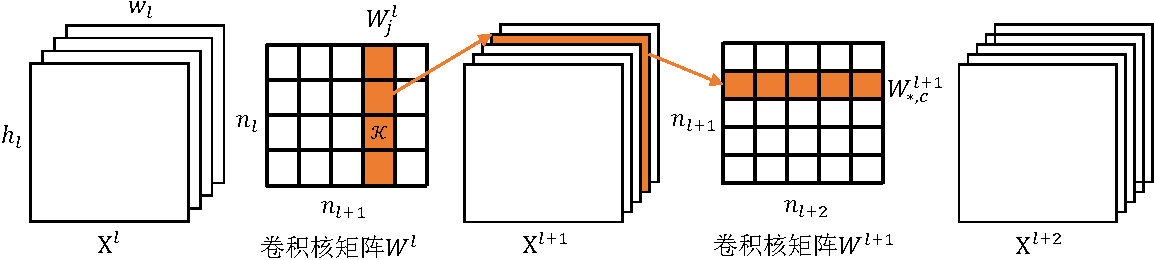
\includegraphics[clip=true, width=0.95\textwidth]{simplify.pdf}
    \caption{移除卷积核对深度卷积神经网络的影响示意图}
    \label{fig:cnn-simplify}
    \vspace{-2em}
\end{figure}

卷积神经网络的简化可以从卷积核、通道以及卷积核内部等多个角度进行稀疏优化。本节
主要研究卷积核的结构化稀疏方法,移除整个卷积核减少模型参数个数,加快模型运算速度。
如图~\ref{fig:cnn-simplify}所示,如果移除卷积核$W^l_j$,
则输出特征图的一个通道$X_j^{l+1}$也被移除,可以减少$n_l k^2 h_{l+1} w_{l+1}$的运算量。
由于输出通道数的减少,下一层卷积层也可以减少一个维度的卷积核,
进一步减少$n_{l+2}k^2h_{l+2}w_{l+2}$的运算量。
已有算法通常采用组稀疏的方法实现结构化稀疏:
\begin{equation}
    W^* = \argmin_{W} \L(X;W) \text{\quad s.t. \quad} \sum_{j=1}^{n_l}\|W_j^l\|_2^p \leq
    \lambda_l, \forall l \in [1,L]
\end{equation}
其中$p$取$0$时为$L_0$约束,取$1$时为$L_1$约束。组稀疏优化相对比较复杂,
$L_0$约束是非凸优化,$L_1$约束不能显示地控制卷积核的个数。
因此,本文提出了基于在线特征选取的深度卷积神经网络模型简化方法。

\subsection{基于在线特征选取的模型简化}
目前,深度网络的训练采取在线优化方法,本节提出将在线多维组稀疏优化问题转化为
一维在线特征选取问题,实现模型简化。如图~\ref{fig:cnn-simplify-w}所示,
在卷积层后引入辅助权重层,权重层参数是对应特征图每个通道的一维卷积核权重向量。
引入辅助权重层以后,模型简化问题的目标函数为:
\begin{eqnarray}
    W^* = \argmin_{W} \L(X;W,\bm{\omega}) \\
    \text{s.t.} \quad
    \sum_{j=1}^{n_l}(\omega_j^l)^0 \leq \lambda_l,
    -1 \leq &\omega_j^l& \leq 1,
    \forall l \in [1,L].
\end{eqnarray}
辅助权重层的前向运算为:
\begin{eqnarray}
    Z_j^l &=& \sum_{c=1}^{n_l}{W_{j,c}^l \ast X_c^l} \\
    X_j^{l+1} &=& Z_j^l \cdot \Omega_j^l \\
    \Omega_{j,:,:}^l &=& \omega_j^l.
\end{eqnarray}

初始条件下所有卷积核的权重$\omega_j^l$为$1$,模型训练过程中更新权重,
每次更新后利用在线特征选取算法保留部分权重并将剩余权重设为$0$,设为$0$的
权重对应的卷积核响应不能传递到更深的网络,因而在模型收敛以后可以将对应的卷积核移除,实现模型简化。
在线特征选取算法可以在训练过程中动态调整需要保留的卷积核,减小模型简化对模型性能的影响。

\begin{figure}[t]
    \centering
    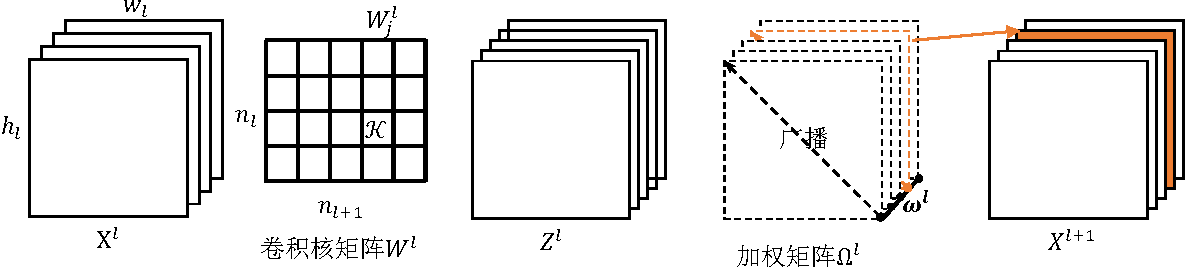
\includegraphics[clip=true, width=0.95\textwidth]{simplify-w.pdf}
    \caption{深度卷积神经网络辅助权重层模型简化}
    \label{fig:cnn-simplify-w}
    \vspace{-2em}
\end{figure}

模型简化问题中梯度通过反向传播得到。假设反向传播到
第$l$层权重层的梯度为$G^{l+1} \in \R^{n_{l+1} \times h_{l+1} \times w_{l+1}}$,
传回第$l$层卷积层的梯度为$\nabla Z^l$,第$l$层权重层的梯度为$\nabla\bm{\omega}^l$,
权重层参数的二阶对角协方差矩阵为$\Sigma^l$,梯度反向传播方式为:
\begin{eqnarray}
    \nabla Z^l &=& G^{l+1} \cdot \Omega^l \\
    \nabla \Omega^l &=& G^{l+1} \cdot Z^l \\
    \nabla{\omega_j}^l &=& \Sigma^l_j\sum_h\sum_w\nabla \Omega^l_{j,h,w} \\
    (\Sigma^l_j)^{-1} &=& (\Sigma^l_j)^{-1}  + \frac{\sum_h\sum_w Z^l_{j,h,w}}{\gamma}.
\end{eqnarray}

\subsection{实验结果和评估}
本文在Cifar10数据集上利用批量归一化(Batch Normalization, BN)的VGG模型(VGG-BN)
研究卷积层简化对于模型准确率的影响~\cite{vggbncifar}。
根据Sergey等人的结果,该模型在Cifar10上达到了$92.45\%$的准确率~\cite{vggbncifar}。
VGG-BN网络包含13层卷积层和2层全连接层,网络结构如表~\ref{tab:vgg-bn-network}所示,参数个数为15M。

本实验首先在Cifar10数据集上预训练VGG-BN网络,达到了$92.78\%$的准确率,然后在
预训练的模型上进行模型简化。简化在Cifar10训练数据集上使用$0.01$的学习率继续训练20轮。

图~\ref{fig:sofs-cnn-simplify}显示了简化不同卷积层对网络准确率的影响。可以发现,深层次的网络存在更多的参数冗余。
对于最深的6层卷积层(conv4\_1至conv5\_3),即使移除了95\%的卷积核,模型的准确率几乎不受到影响。
根据表格~\ref{tab:vgg-bn-network}中结果,最深的卷积层占据了主要的参数个数。因此,稀疏简化这些层能够显著减少
模型的大小和计算量。此外,可以发现随着网络深度的减小,卷积层对于简化的敏感性也逐渐增强。一方面可能是由于浅层卷积层
的卷积核个数本身比较少,另一方面可能是由于浅层网络提取更多的浅层语义,Cifar10数据集的内容比较简单,
深层次语义对于图片分类提升作用相对较小,因而对于模型简化的敏感性也较低。

\begin{table}[t]
    \centering
    \caption{VGG-BN网络结构}
    \label{tab:vgg-bn-network}
    \footnotesize
    \begin{tabular}{|c|c|c|c|c|c|c|c|c|c|}
        \hline
        卷积层 & 输入大小 & 卷积核数目 & 参数个数 & 卷积层 & 输入大小 & 卷积核数目 & 参数个数 \\ \hline
        conv1\_1 & 32x32 & 64 & 1,792 & conv4\_1 & 4x4 & 512 & 1,180,160 \\ \hline
        conv1\_2 & 32x32 & 64 & 36,928 & conv4\_2 & 4x4 & 512 & 2,359,808 \\ \hline
        conv2\_1 & 16x16 & 128 & 73,856 & conv4\_3 & 4x4 & 512 & 2,359,808 \\ \hline
        conv2\_2 & 16x16 & 128 & 147,584 & conv5\_1 & 2x2 & 512 & 2,359,808 \\ \hline
        conv3\_1 & 8x8 & 256 & 295,168 & conv5\_2 & 2x2 & 512 & 2,359,808 \\ \hline
        conv3\_2 & 8x8 & 256 & 590,080 & conv5\_3 & 2x2 & 512 & 2,359,808 \\ \hline
        conv3\_3 & 8x8 & 256 & 590,080 & 总计 & - & 4224 & 14,714,688 \\ \hline
    \end{tabular}
\end{table}
\begin{figure}[t]
    \center
    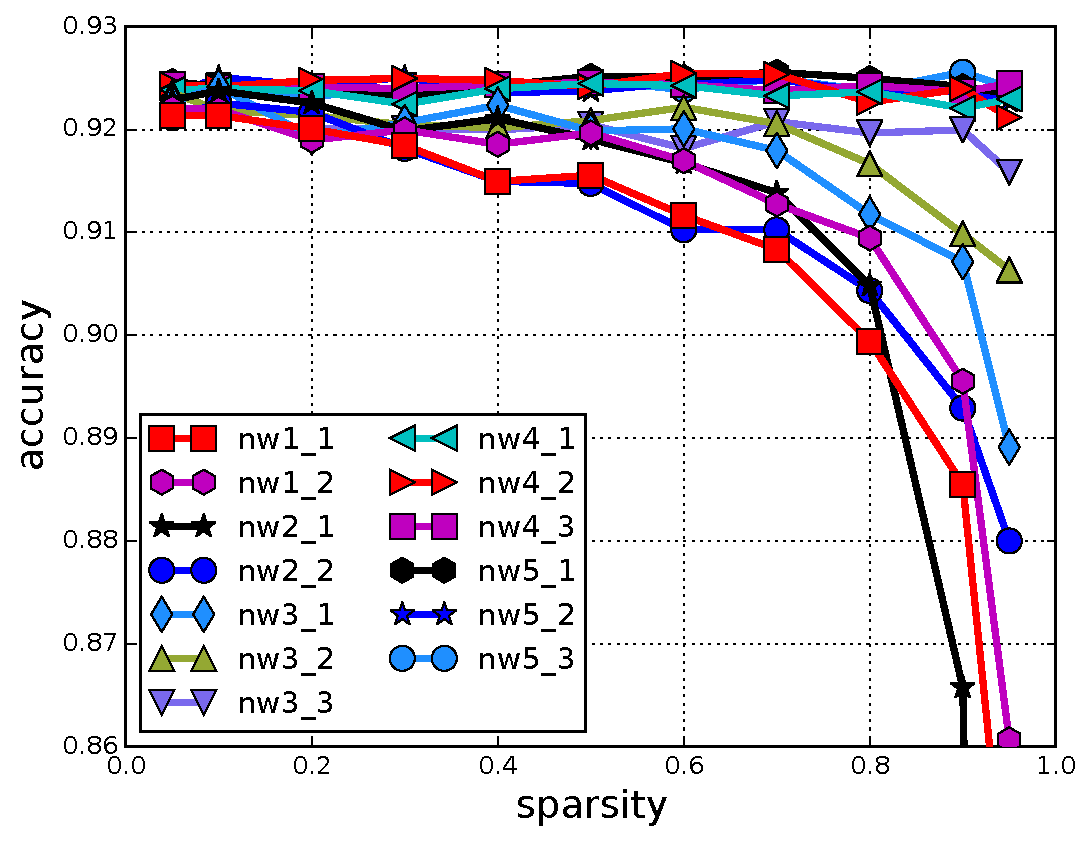
\includegraphics[clip=true, width=0.9\textwidth]{sofs-cnn-simplify.pdf}
    \caption{模型简化对模型准确率的影响}
    \label{fig:sofs-cnn-simplify}
    \vspace{-2em}
\end{figure}

为了更清晰地表示不同卷积层受模型简化的影响,表~\ref{tab:vgg-bn-layer-sparsity}显示了在
模型准确率下降至原来的99\%,95\%和90\%时不同层对应的稀疏度。当可容忍的准确率下降比例为1\%时,前7层卷积层能达到60\%左右的稀疏度,
后6层能达到95\%的稀疏度。随着可容忍下降比例的提高,网络的稀疏度也迅速增加,到10\%的下降比例时,
几乎所有层都能达到95\%的稀疏度或更高。

\begin{table}[t]
    \centering
    \caption{VGG-BN网络不同卷积层在不同准确率下的稀疏度($\rho$为下降百分比)}
    \label{tab:vgg-bn-layer-sparsity}
    \footnotesize
    \tabcolsep=1.6mm
    \begin{tabular}{|c|c|c|c|c|c|c|c|c|c|c|c|c|c|}
        \hline
        $\rho$  & C1\_1 & C1\_2 & C2\_1 & C2\_2 & C3\_1 & C3\_2 & C3\_3 & C4\_1 &  C4\_2 & C4\_3 & C5\_1  & C5\_2 & C5\_3 \\ \hline
        0.01  & 60\% & 60\% & 40\% & 40\% & 60\% & 70\% & 90\% & 95\% &  95\% & 95\% & 95\%  & 95\% & 95\% \\ \hline
        0.05  & 90\% & 90\% & 80\% & 90\% & 95\% & 95\% & 95\% & 95\% &  95\% & 95\% & 95\%  & 95\% & 95\% \\ \hline
        0.10  & 95\% & 95\% & 90\% & 95\% & 95\% & 95\% & 95\% & 95\% &  95\% & 95\% & 95\%  & 95\% & 95\% \\ \hline
    \end{tabular}
\end{table}

%为了在所有层上进行模型简化,本实验从浅层网络依次向深层网络进行简化,并将前一层简化结果
%中不低于92\%的准确率的最稀疏模型作为为下一层模型简化的预训练模型。最终简化结果如所示。

\section{本章小结}
本章主要解决大规模高维特征选取问题和深度卷积神经网络模型简化问题。
特征选取是从所有特征中选取一小部分与具体问题相关的特征。
本章提出了一个新的二阶在线特征选取算法SOFS。区别于已有在线特征选取
算法的复杂度与特征维度成正比,本章提出的算法的复杂度被显著减少到与每个训练样本的
非零特征个数成正比。本章在中等规模和大规模的合成数据集和真实数据集上进行了
充分实验,比较所提出算法相对于当前最好的批处理算法和在线特征选取算法的有效性和高效性。
实验结果表明SOFS算法不仅能够显著减少训练的训练时间,
还可以达到当前最好的批处理算法相近甚至更好的准确率,
使得SOFS算法成为处理大规模高维数据的切实可行的特征选取算法。

此外,本章提出了深度卷积神经网络模型简化算法,将传统的多维卷积核组稀疏优化问题转化为一维特征选取问题,
并基于在线特征选取算法给出了有效的模型简化方案。实验部分分析了不同网络卷积层
对于模型简化的敏感性,充分证明了模型简化的有效性。

本章的主要贡献包括:
\vspace{-0.5em}
\begin{itemize}\setlength{\itemsep}{0em}
    \item 提出了高效的二阶在线特征选取算法,用于解决大规模高维稀疏数据的特征选取问题。
    \item 提出了快速一阶在线特征选取算法和快速二阶在线特征选取算法,尤其是二阶算法的
        复杂度从与所有维度成正比降低到与非零特征个数成正比。
    \item 提出了高效的深度卷积神经网络模型简化算法,将多维卷积核组稀疏优化问题转化为一维特征选取问题。
    \item 进行了充分的实验,验证了所提出算法的有效性和高效性。
\end{itemize}


\chapter{基于主题的照片集故事化表达}
随着智能手机和智能移动设备的普及,人们几乎可以在任意时间任意地点拍摄照片。
大量的照片被分享到社交网络以后,用户很少再次浏览或利用这部分数据,
原因在于当前的社交多媒体缺少智能的服务去组织和挖掘用户数据。因此,
本章提出一个基于主题的照片集故事化表达系统——Monet,总结整理用户照片集,
并以故事化的表现形式重现照片集中的场景和事件。

本章首先介绍照片集故事化表达面临的主要问题和Monet系统的主要框架,然后依次介绍系统的两个
主要组成部分:照片集分析与梳理和照片集故事合成,最后通过实验验证本章所提出系统的有效性。

\section{主要问题与系统框架}
从照片集中总结生成有吸引力和纪念意义的故事化表达面临一些挑战。首先,海量的用户照片集通常
是无序的,浏览和分享照片的过程十分枯燥。然而大部分情况下,用户照片不是随机拍摄的,
而是拍摄在不同事件的特殊时刻。对于故事化表达系统,挖掘照片集中的事件并将照片集按照事件进行组织
十分必要。其次,用户会在事件中拍摄较多内容相似的照片,照片集存在数量多内容冗余的问题。
此外,由于普通用户不具备专业的拍摄技术,很多用户照片存在质量较差的问题。
因此,从照片集中选取一部分有代表性的子集是照片集故事化表达的关键步骤。
再次,故事化表达系统需要将选取的照片用有吸引力的方式重新呈现给用户,提升用户体验。
在本章提出的系统中,照片集通过音乐视频的方式表达。由于照片拍摄在不同的场景,系统
需要自动选取合适的编辑风格达到不同的表达效果。最后,为了增加音乐视频的吸引力,
应该在视频渲染时引入视频编辑元素,如视频特效、形状、颜色过滤器、转场等。
从专业的视频编辑的角度,这些编辑元素依赖特定的内容和风格。因此,如何挖掘视频编辑语法,
设计基于风格的编辑元素,并将它们运用到故事化表达系统中是一项具有很大挑战但又十分必要的部分。

根据以上总结的主要问题,本章提出的基于主题的照片集故事化系统如图~\ref{fig:monet-framework}所示。
系统首先检测照片集中的事件,然后在每个事件中选取一部分关键照片,完成对照片集的分析与梳理。
在选取的关键照片上,系统自动为每张照片选取合适的编辑风格。根据预先定义的编辑语法,
系统结合相机运动,视频特效和音乐产生视频片段。最后,通过在视频片段之间添加转场效果产生
完整的音乐视频。系统的每个部分将在后续章节逐一介绍。
\begin{figure}[t]
    \center
    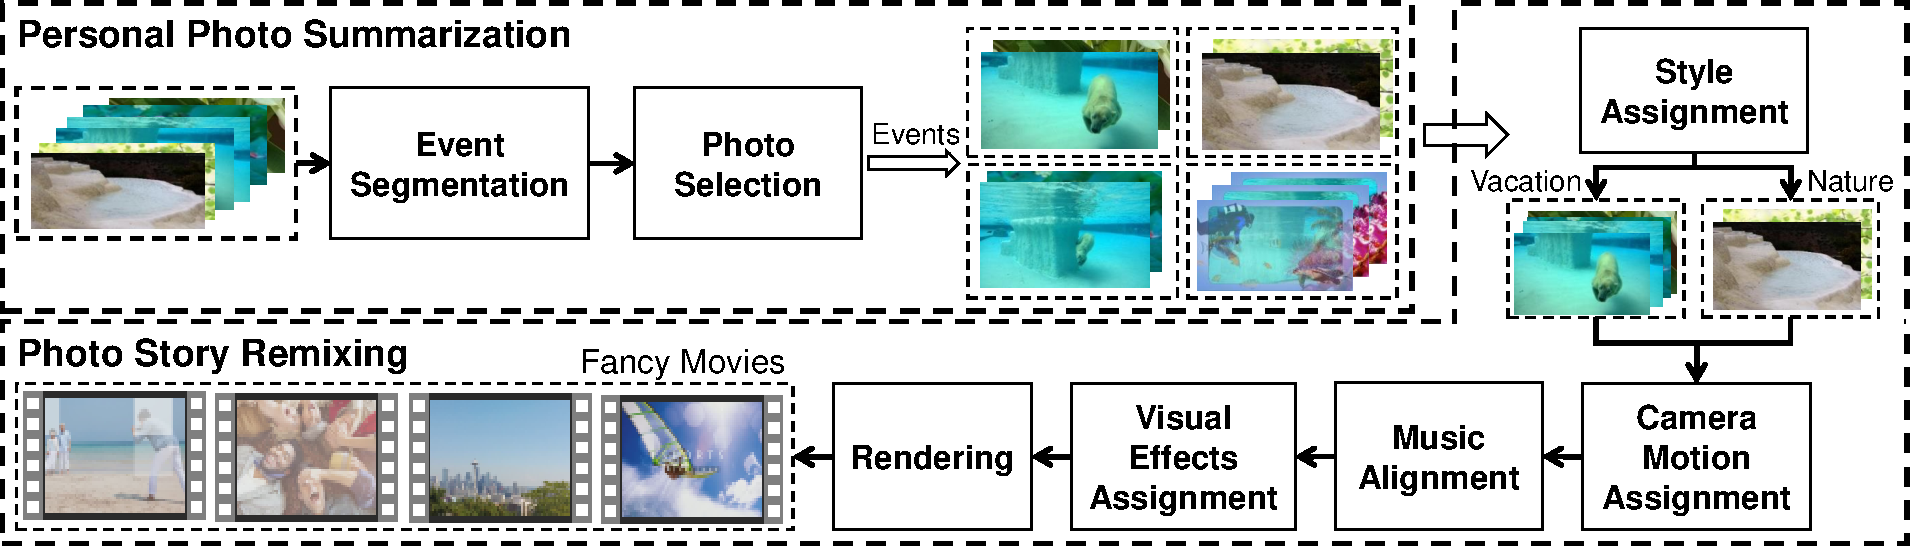
\includegraphics[clip=true, width=0.95\textwidth]{monet-framework.pdf}
    \caption{基于主题的照片集故事化表达系统框架}
    \label{fig:monet-framework}
    \vspace{-2em}
\end{figure}

\section{照片集分析与梳理}
照片集分析与梳理包含两个步骤:事件检测和照片筛选。事件检测将照片按照事件进行组织。
照片筛选首先移除低质量或者重复的照片,然后选取高质量的有代表性和均衡性的照片子集
作为关键照片。

\subsection{事件检测}
从统计上看,用户倾向于在集中的时间点拍摄照片。为了清楚地解释事件检测的概念,本章定义
``事件''如下:
\begin{definition}[\textbf{事件}]
    事件是特定的情景下、相对较短的时间段内,用户记录值得留念的时刻的一组拍摄行为。
\end{definition}

因此,同一事件中的照片在时间和地点上比较接近。
用$N$和$K$分别代表照片集$\X$中照片和事件的数目,
每个照片$\x_i \in \X = \{\x_1, \x_2, \ldots, \x_N\}$属于事件$e_j \in E = \{e_1, e_2, \ldots,
e_K\}$的概率可以表示为$p(\x_i|e_j)$,$\x_i=(x_{i,1},
x_{i,2})$,$x_{i,1}$是时间($\mathcal{T}$),
$x_{i,2}$是GPS($\mathcal{G}$)。如果$p(e_j|\x_i)$是最大后验概率,则$\x_i$被判定
属于事件$e_j$。

给定事件$e_j$,假设时间和位置信息之间是独立的,似然函数$p(\x_i|e_j)$表示为:
\begin{equation}
    \label{equ:monet-priori}
    p(\x_i|e_j)= \prod_{l=1}^{2}p(x_{i,l}|e_j) = p(\mathcal{T}_i | e_j)p(\mathcal{G}_i | e_j).
\end{equation}
每个$x_{i,l}$相对于事件$e_j$的概率服从高斯分布:
\begin{equation}
    p(x_{i,l}|e_j) =
    \frac{1}{\sqrt{2\pi\delta_{j,l}^2}}e^{-\frac{(x_{i,l}-\mu_{j,l})^2}{2\delta_{j,l}^2}}.
\end{equation}
事件检测的过程其实是学习方程~\eqref{equ:monet-priori}中混合高斯模型(Gaussian Mixture Model, GMM)
参数的过程$\Theta=\{\delta_{j,l}, \mu_{j,l}\}, j\in[0,K-1], l\in\{1,2\}$。优化的目标方程是如下所示联合概率的对数似然函数:
\begin{equation}
    \label{equ:monet-likeli}
    l(\X;\Theta)= \log(\prod_{i=1}^N p(\x_i|\Theta)) =
    \sum_{i=1}^N \log(\sum_{j=1}^K p(e_j)p(\x_i|e_j,\Theta)),
\end{equation}
$p(\x_i|e_j,\Theta)$通过方程~\eqref{equ:monet-priori}计算得到,
$p(e_j)$是事件$e_j$的先验概率。本章提出的系统使用EM算法学习最优参数。
系统用K-means算法的聚类中心初始化GMM模型的参数。
为了决定事件的数目$K$,系统在不同数值的$K$上运用EM算法,
产生一系列可能的事件分割结果。最优事件数目通过Tao等人提出的最小描述长度
(Minimum Description Length, MDL)决定~\cite{mei2006probabilistic}。

\subsection{照片筛选}
由于照片集中照片数量较多,并且多数照片是由没有专业拍摄技巧的普通用户拍摄的,
系统需要滤除低质量和重复的照片,并进一步选取高质量、有代表性和均衡性的照片子集,
得到照片集高质量的故事总结。

\textbf{质量过滤}:
由于欠曝光、过曝光、模糊等问题,照片的质量可能十分低下。本章提出的Monet系统用$43$维
人工设计的特征评价照片质量,包括:
\begin{itemize}\setlength{\itemsep}{0pt}
    \item 暗度(1D),亮度(1D):欠曝光和过曝光的像素比例~\cite{qa_bright};
    \item 模糊度(1D)~\cite{qa_blur},模糊差异(1D)。
        模糊差异是指照片的模糊度与照片经过高斯模糊后的模糊度之间的差值。
    \item 锐度(2D)~\cite{qa_blur,qa_sharpness},复杂性(1D)~\cite{qa_sim},
        对比度(1D)~\cite{qa_dyn_range}, 动态范围(1D)~\cite{qa_dyn_range},
        景深(1D)~\cite{qa_zhedong}。这些特征是常见的照片质量评估的全局特征。
    \item HSV分布(12D)~\cite{qa_hsv}。首先将照片转换到HSV颜色空间,然后用
        非均匀量化将``hue''量化为8份,将``value''量化为4份。
    \item 最好块特征(7D),最差块特征(7D),主体块特征(7D)。通过观察发现,某些情况下只有
        照片的一部分存在质量问题,导致整张照片被认为是低质量照片,
        此时全局特征并不能充分表示这种情况。因此系统将照片分成$5$个块(左上角、
        右上角、左下角、右下角和中间),从具有最大对比度、最小对比度和中间块提取
        常用的全局特征。
\end{itemize}

我们收集了一个包含$10,361$张高质量照片和$3,134$张存在质量问题的照片的数据集,所有照片都
来自于用户拍摄的真实照片,并被人工标注为``good''或``bad''。利用上述43维特征,
我们在这个数据集上训练SVM分类器。照片质量通过SVM模型预测的边界值评估,质量分数低于特定
阈值的照片将会被移除。

\textbf{重复照片过滤}:为了更好地梳理照片集,需要检测内容重复的照片,
并只保留每组内容重复照片中美学质量最高的照片。系统采用了Winder等人提出的局部特征将每张照片表示为$64$
维向量~\cite{t2s2},向量的每个维度都是一个整数。照片的相似度定义为两个向量之间相同整数的个数。
如果相似度大于某个阈值,则认为是重复照片。

\textbf{关键照片选取}:为了选取一部分照片子集作为关键照片代表整个照片集,
系统考虑三个因素:美学质量、代表性和均衡性。
\vspace{-0.5em}
\begin{itemize}
    \item \textbf{美学质量}:专业的视频制作需要选取美学质量很高的照片素材。
        本章采用了Dong等人提出的模型评价照片的美学质量~\cite{dong2014eepqa}。
    \item \textbf{代表性}:照片的代表性从两个方面进行评价:(1)照片所在事件的
        重要性。当用户对某个事件更加感兴趣时,通常拍摄更多的照片,反之亦然。
        因此,对于事件$e_i$,如果事件中的照片数目为$n_i$,整个照片集中照片的数目为
        $N$,则事件$e_i$的重要性为$\mathcal{EI}_i=\frac{n_i}{N}$;(2)多样性。
        系统从事件中选取多样性最大的照片子集。通过提取照片的时间信息($\t \in
        R^1$), 位置信息($\l \in R^2$)和颜色直方图($\c\in R^{64}$),
        照片$\x_i$和$\x_j$之间的距离定义为:
        \begin{equation}
            d_{ij} = dist(\t_i, \t_j) + dist(\l_i, \l_j) + dist(\c_i, \c_j),
        \end{equation}
        其中$dist(\a,\b)=exp(-\frac{\|\a-\b\|^2}{\sigma^2})$。

        对于照片$\x_i$,多样性定义为$\mathcal{D}_i = \sum_j d_{ij}I_{j}$。
        $I_j$是一个指示函数,当$x_j$被选为关键照片时$I_j=1$,否则$I_j=0$。
        因此,照片$x_i$的代表性为:
        \begin{equation}
            \mathcal{R}_i=\mathcal{EI}_i + \mathcal{D}_i
        \end{equation}
    \item \textbf{均衡性}:美学质量和代表性是从照片的内容上进行关键照片选取,
        为了获得对照片集更加综合的总结概括,照片在时间上的均衡性也是一个重要的因素。
        系统利用照片之间的时间间隔的熵作为均衡性的表示。假设照片$\x_i$与$\x_i$前一个被选取的
        照片和下一个被选取的照片之间的时间间隔为$t_{i,i-1}$和$t_{i,i+1}$,$\x_i$的熵定义为:
        \begin{eqnarray}
            \mathcal{E}_i=t_{i,i-1}\log t_{i,i-1} + t_{i,i+1}\log t_{i,i+1}
        \end{eqnarray}
\end{itemize}
照片被选取的适合度是上述三个因素的线性组合:
\begin{equation}
    S_i = a \mathcal{Q}_i + b \mathcal{R}_i + c \mathcal{E}_i.
\end{equation}
其中,$a,b,c$是满足$a+b+c=1$的非负加权参数。由于代表性和均衡性依赖于整体选取的照片,
系统很难获取到关键照片选取的全局最优解。因此,系统用贪心算法获得关键照片子集。

\section{照片集故事合成}
视频制作通常包括6个步骤:(1)选取合适的编辑风格和背景音乐;(2)基于选取的风格添加照片;
(3)为每个静态照片设计运动效果将其转化为视频片段;(4)对每个片段运用相机运动、形状、
颜色过滤器、文本等视觉特效;(5)为相邻片段选取转场效果;(6)组合所有的片段和转场效果,
添加开场和结束效果生成最终的音乐视频。
一般来说,设计师需要决定编辑风格,并根据素材的语义内容设计视觉效果。

仿照上述专业视频制作的步骤,本节首先分析照片的语义内容。基于照片的内容,
系统为不同照片分配不同的编辑风格,并选取合适的相机运动、视觉特效和转场等效果。

\vspace{-1em}
\subsection{语义理解}
在视频制作过程中,素材的语义特征和内容对于风格选取、运动设计,特效制作十分重要。
Monet系统采用了本论文提出的社交多媒体数据语义理解方法提取照片的语义特征。
每张照片$\x_j$有$112$个可能的标签($t_i$)以及相应的概率$P(t_i|\x_j)$,
这些标签和概率将会用来判断照片的编辑风格。

为了定义每个编辑风格可计算的编辑语法,这些标签被分成$20$个常见的用户照片类别,包括\emph{动物、建筑、暗黑、
食物、室内、室外、物体、人物、多人、人群、植物、天空、文本、山}和\emph{建筑}。
此外,人脸对于用户照片格外重要,系统检测照片中人脸的数目、性别、大小和位置。
照片里的人脸特征分为``侧脸''、``一两个大比例人脸''、``一两个小比例人脸''、``三到五个小比例人脸'',``一组
小比例人脸''和``一组大比例人脸''。性别信息包括``单个人''、``单个男性''、``单个女性''、
``两个女性''、``两个男性''、``两个男性''、``夫妻''和``人群''。所有这些特征信息将用于后续
的生成视频片段和选取视觉特效等步骤。

\subsection{风格选取}
本节讨论如何将照片聚类到场景以及如何为这些场景选择合适的编辑风格,
风格选取的流程如图~\ref{fig:style-assignment}所示。
\begin{figure}[t]
    \centering
    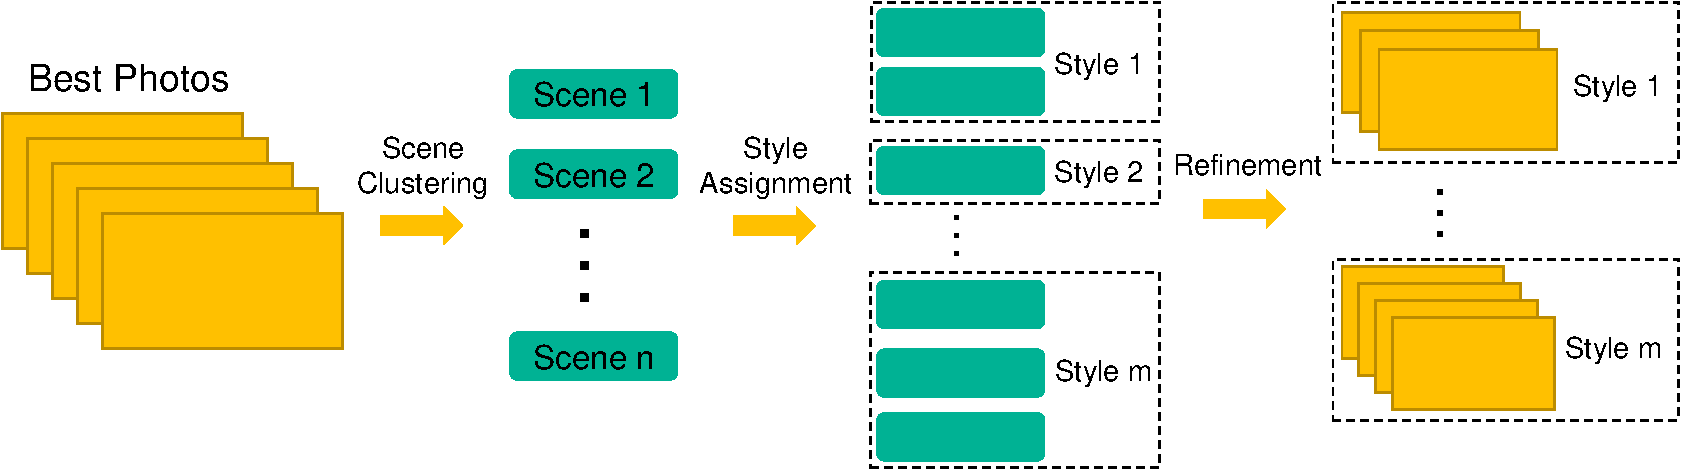
\includegraphics[clip=true, width=0.95\textwidth]{style-assignment.pdf}
    \caption{风格选取流程}
    \label{fig:style-assignment}
    \vspace{-2em}
\end{figure}

\textbf{场景聚类}:根据我们与设计师讨论的结果,用户通常在特定的场景中拍摄照片记录值得
纪念的时刻。换句话说,照片不仅被时间和位置信息显式地组织,同时也被场景隐式地组织。
本章提出的系统的主要目的是从用户照片中总结场景并生成音乐视频。为了衔接照片和场景之间的联系,
每个照片用上节阐述的语义模型对应的概率向量表示$\p_i = (P(t_1|x_i), P(t_2|x_i), \ldots,
P(t_N | x_i))$。我们用Affinity Propagation~\cite{frey2007clustering}算法对照片聚类,
每个聚类中心被当做是一个场景。

\textbf{风格选取}:在本章系统中,用不同的编辑风格表现不同的场景,使得故事化的表达
更加智能更加具有吸引力。为了定义不同的编辑风格,
我们邀请设计师设计了用户照片中最常见的主题风格以及相关的语义词汇,如
``爱情''相关的词汇包括\emph{爱情、夫妻、甜蜜、婚礼、宝贝}等。为了使得这些词汇表达的语义
是可计算的,我们用这些词从Flickr上获取至少$5,000$张照片,并用本文提出的语义理解模型和
特征选取算法提取照片的语义特征,训练多类SVM分类器区别不同的风格。
相应的,照片$\x_k$属于风格$\S_j$的概率表示为$P(\S_j|\p_k)$。

如果场景$scene_i$包含$M$张照片,$scene_i = \{\p_1^i, \p_2^i, \ldots,
\p_M^i\}$,该场景属于风格$\S_j$的概率为:
\begin{equation}
    P(scene_i, \mathcal{S}_j)= \sum_{k=0}^{M-1} P(\mathcal{S}_j|\textbf{p}_k^i) / M.
\end{equation}
最终,系统选取概率最大的风格编辑场景$scene_i$。
系统可能会给不同的场景选择相同的编辑风格,
相同风格的照片将被合并到一起生成一个音乐视频。

\subsection{生成视频片段}
Monet系统采用了Hua等人提出的从照片生成视频片段的方法~\cite{hua2006photo2video},
主要包括三个步骤:
\begin{itemize}\setlength{\itemsep}{0pt}
    \item 关键帧选取。为了模拟相机运动,需要在照片中选取全景、中景和近景作为关键帧。
    \item 生成关键帧序列,决定关键帧的播放顺序。基于电影制作的规则,系统采用了
        Hua等人提出的14种播放策略产生关键帧序列~\cite{hua2006photo2video}。
    \item 生成相机运动。最终的视频片段通过在关键帧之间采用特定的相机运动实现。
        按照Hua等人提出的方法,系统构建了一个相机运动和关键帧之间的合适度矩阵,通过
        最大化相机运动合适度和相机运动分布均衡性为每个照片选取合适的相机运动。
\end{itemize}

\subsection{音乐分析}
音乐视频需要将视频镜头切换和音乐节奏进行匹配。Monet系统首先将音乐频率采样到8kHz,
并通过Hua等人提出的方法检测音乐的节奏~\cite{hua2006photo2video}。
根据音乐的节奏和强度,系统检测最终音乐视频的切换点,决定视频片段的时长。
切换点是指音乐视频从一个视频片段切换到另一个视频片段的时间点。
切换点的检测算法将在~\ref{sec:mashup-cutpoint}节中详细阐述。相比于已有的切换点检测算法,
该方法提供了更好的音视频关联性,视频片段的切换频率和音乐节奏更加协调。

\subsection{故事合成}
专业的音乐视频需要对视频片段添加视频特效、形状、 颜色过滤器、转场等视觉效果,
使得音乐视频更加平滑更加具有吸引力~\cite{mei2007videosense}。
我们为每个主题风格总结了可计算的视频编辑语法并设计了风格模板,
将视觉效果添加到视频片段中。最终的音乐视频根据视频片段、音乐和视觉特效生成。

\subsubsection{风格模板设计}
对于每个风格,我们设计了视频特效、形状、颜色过滤器和转场效果,每个视觉效果都依赖具体
的照片内容。图~\ref{fig:monet-shape_et_example}显示了一些视觉效果的样例。
\begin{figure}[t]
    \centering
    \subfigure[条纹效果] {
        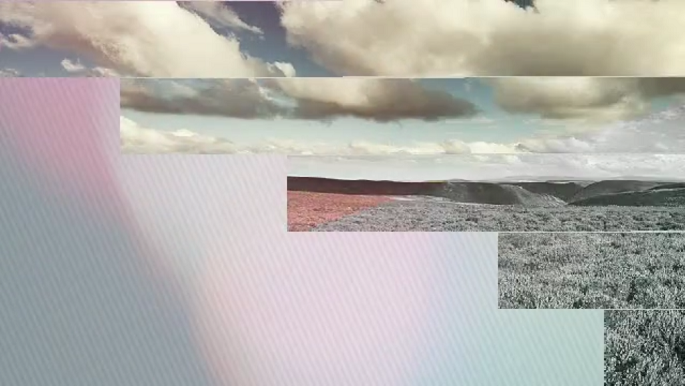
\includegraphics[width=0.23\linewidth]{multi-stripe.png}
    }
    \subfigure[叶子形状] {
        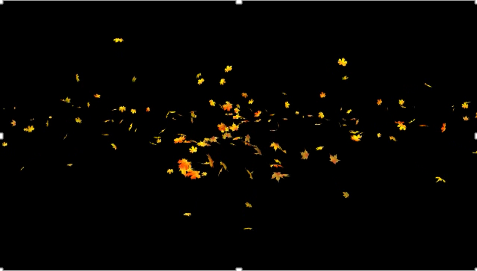
\includegraphics[width=0.23\linewidth]{shape.png}
    }
    \subfigure[阳光颜色过滤器] {
        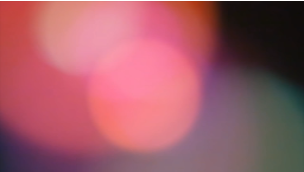
\includegraphics[width=0.23\linewidth]{color-filter.png}
    }
    \subfigure[圆形转场] {
        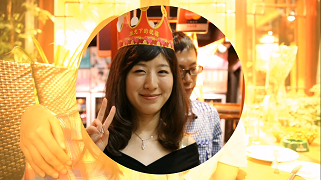
\includegraphics[width=0.23\linewidth]{transition.png}
    }
    \caption{视频特效、形状、颜色过滤器和转场样例}
    \label{fig:monet-shape_et_example}
    \vspace{-2em}
\end{figure}

不同的视觉效果有不同的表达效果,适用于不同的语义内容。比如,
图~\ref{fig:monet-shape_et_example}(a)中的条纹效果将照片分割成条纹依次展现,是``自然''主题风格的一种表现手法。
该效果适用于户外拍摄的植物或天空,但不适用于包含人物的照片,因为没有用户愿意人物照片
被分割成条纹。图~\ref{fig:monet-shape_et_example}(b)的叶子形状中,
黄色的树叶缓慢地漂浮在视频中,唤醒用户对于原始和旧时光的记忆,适用于包含草地或者树叶的照片。
图~\ref{fig:monet-shape_et_example}(c)的阳光颜色过滤器
将照片和阳光颜色过滤器融合,能够帮助用户体验自然主题下的阳光照耀的效果。
在图~\ref{fig:monet-shape_et_example}(d)中,``聚会''风格的圆形转场逐步从中间到四周
展现内容,能够有效地吸引观看者的注意力到照片中的主要物体或人物,特别适合照片中间仅有
一个焦点人物或物体的照片,尤其是仅包含大比例人脸的照片。
视觉效果的选取除了与照片内容相关,某些效果尤其是转场效果仅适用于特定的相机运动。总之,不同的视觉效果对于不同的语义内容和相机运动有不同的
合适度,我们为每个风格的视频特效、形状、颜色过滤器和转场定义了合适度语法。特效的语法规则定义
为如下xml格式(形状和转场的语法类似):
\begin{itemize}\setlength{\itemsep}{0pt}
    \item \textbf{根节点$<$Grammar$>$}:根节点包含风格信息以及视频特效、形状、颜色过滤器和转场语法的子节点。
    \item \textbf{特效节点$<$Effect$>$}:特效节点描述视觉效果相对于不同语义特征和运动的合适度。
        每个特效节点包含一个或者多个``condition''子节点和一个可选的``percent''子节点。
        ``condition''节点包含``feature''和``score''两个子节点。如果``feature''节点以``+''
        开头,则该特效适用于该特征,如果以``-''开头,则特效不适用。``score''子节点表示特效
        适用于该特征的程度。特效节点的``percent''子节点表明该特效在所有选择特效中
        适宜出现的比例。如果视频片段包含不适合的特征,特效的合适度为$0$,
        否则特效的合适度为所有特征合适度之和。
\end{itemize}

根据特效语法,可以计算出每个视觉效果和每个视频片段的合适度以及部分效果期望出现的比例。

颜色过滤器的语法稍有不同。即使对于相同的视频片段,
光照和颜色分布的变化也会导致不同的表达效果。
因此,我们为不同的风格设计了不同的颜色过滤器,语法格式为:
\begin{itemize}\setlength{\itemsep}{0pt}
    \item \textbf{视频颜色过滤器节点$<$ColorFilter$>$}:该节点描述以视频形式出现的
        颜色过滤器的语法。``path''子节点包含视频的路径,``opacity''子节点控制过滤器视频和
        视频片段叠加时的不透明度,``overlay''子节点包含叠加的方式,``minPercent''和``maxPercent''
        控制该视频过滤器出现的最少和最大比例。
    \item \textbf{图片颜色过滤器节点$<$ImageFilter$>$}:该节点描述图片颜色过滤器的语法。
        节点内容与视频颜色过滤器基本相同,除了``path''子节点被替换为``name''子节点,表明预先定义的
        图片颜色过滤器名称。此外,图片颜色过滤器节点包含\textbf{特效节点$<$Effect$>$}节点中的``condition''节点。
\end{itemize}

为了计算视频颜色过滤器和视频片段之间的合适度,系统首先提取颜色过滤器视频和视频片段的显著图(Saliency
Map)~\cite{ma2003saliency},合适度通过显著图之间的负相关系数得到。换句话说,视频颜色过滤器
不应该将用户的注意力从照片的主题内容分散到颜色过滤器上。

\subsubsection{视觉效果选取}
视觉效果选取定义为一个优化问题进行求解。假设一共有$N_c$个视频片段,每个视频片段表示为$c_i$,一共有$N_e$个视觉效果,
每个表示为$VE_j$。系统通过确定一个选择矩阵$X=(\x_1, \x_2, \ldots, \x_{N_C})$选取视觉效果,
$\x_j$是一个$N_e$维的仅包含一个非零元素的二值向量。由于不同的视觉效果
有不同的期望出现比例(percent),首先需要确定它们的期望选择次数$n_j^*$。
如果$VE_j$的期望比例为$p_j$,显然$n_j^* = p_jN_c$。如果$p_j$没有指定,则根据
它们与视频片段之间的合适度确定出现比例。假设视频片段$c_i$和视觉效果$VE_j$之间的合适度
为$S_{ij}$,$VE_j$的整体合适度为:
\begin{equation}
    S_j = \sum_{i=0}^{N_c-1}S_{ij}(1 - I_j),
\end{equation}
$I_j$是一个指示向量,当$p_j$被指定时$I_j$为1,否则为0。$VE_j$期望出现的比例为:
\begin{equation}
    p_j = \frac{S_j}{\sum_{k=0}^{N_e-1}S_{k}(1 - I_{k})}p^*,
\end{equation}
其中$p^* = 1 -\sum_{k=0}^{N_e-1}p_{k}I_{k}$是没有被指定比例的视觉效果能够出现在视频片段
中的剩余比例。

视觉效果选取定义为最大化整体合适度和出现比例的优化问题:
\begin{equation}
    X^* = \argmax_{X}
    \sum_{j=0}^{N_e-1}d_j\frac{\sum_{i=0}^{N_c-1}X_{ij}S_{ij}}{n_j},
\end{equation}
其中$d_j = exp(-\frac{(n_j-n_j^*)^2}{2})$是出现比例的合适度,
用以衡量视觉效果的出现比例和预期出现比例之间的差异。

然而,仅仅最大化合适度和出现比例可能会导致相同的视觉效果被分配到
连续的视频片段。为了保持视频片段原始的顺序,保证最终视频的故事性,同时防止这种连续
效果的单一性,我们进一步约束视觉效果分布的均匀性。

假设$VE_j$在$N_c$个视频片段中出现$n_j$次,$VE_j$应该均匀地出现在视频中。因此,
选择$VE_j$的相邻视频片段之间的预期间隔为$\frac{N_c -
n_j}{n_j}$。假设选择$VE_j$的第$k$个和第$k+1$个视频片段之间的间隔为$\delta_k$,则$VE_j$
的均匀性分数$u_{jk}$定义为:
\begin{equation}
    u_{jk} = exp(-\frac{(\delta_{k}-\frac{N_c-n_j}{n_j})^2}{2}).
\end{equation}
相应地,整体的均匀性分数为:
\begin{equation}
    U = \sum_{j=0}^{N_e-1}\frac{\sum_{k=0}^{n_j-1}u_{jk}}{n_j^*-1}.
\end{equation}

考虑到合适度、出现比例和均匀性,视觉效果选取问题定义为如下优化目标方程:
\begin{eqnarray}
    X^* = \argmax_{X_{ij}}
    \sum_{j=0}^{N_e-1}(d_j\frac{\sum_{i=0}^{N_c-1}X_{ij}S_{ij}}{n_j}
    + \lambda \frac{\sum_{k=0}^{n_j-1}u_{jk}}{n_j^*-1}).
\end{eqnarray}
系统使用回溯法求解上述优化方程。

经过对用户照片集的事件检测、关键照片选取、视频片段生成、音乐匹配以及视觉效果选取,
Monet系统生成最终的音乐视频,完成对用户照片集的分析梳理,并按照主题对用户照片集进行故事化的表达。

\section{实验结果和评估}
据了解,目前还没有其他完整的系统能够自动对用户照片集进行分析与梳理并创建故事化的表达。
为了评价Monet系统的有效性,本节从照片集分析与梳理和照片集故事合成两个角度评价Monet系统。

在实验中,所有的实验数据都从用户上传的照片集中选取。为了评价照片集分析与梳理的效果,
我们让上传者对他们的照片进行标注,找出照片集中的事件和关键照片,并将用户照片上传到
其他事件检测和关键照片选取系统,获取它们分析与梳理结果。对于故事合成,我们邀请用户从他们的
照片集中针对每个主题风格推荐照片,然后针对每个风格将对应的照片和音乐提交到
Monet系统和其他系统中,通过用户调查(user study)比较不同系统生成的视频。

\subsection{事件检测和关键照片选取评估}
我们邀请了6名用户分享他们在过去两年拍摄的照片,所有的照片都包含准确的拍摄时间,
但只有一部分包含GPS信息。我们要求用户将他们的照片按照事件分组,
并为每个事件选取最能代表这个事件的1到6张照片作为关键照片。
这些用户标注的结果被当作评测事件检测和关键照片选取的真实数据。照片集的详细情况
如表~\ref{tab:monet-photos-info}所示。
\begin{table}[t]
    \centering
    \caption{用户照片集详细信息} \label{tab:monet-photos-info}
    \begin{tabular}{|c|c|c|c|c|c|c|}
        \hline
        Dataset & User 1 & User 2 & User 3 &  User 4 &User 5 & User 6\\ \hline
        \#Photos & 1080 & 481 & 496 &  564 & 702 & 866 \\ \hline
        \#Events & 95 & 32 & 40 &  107 & 28 & 58 \\ \hline
        \#Best Photos & 206 & 145 & 108 &  375 & 66 & 285 \\ \hline
    \end{tabular}
\end{table}

实验采用了准确率(Precision)、召回率(Recall)和F-score来评测事件检测的效果~\cite{cooper2005temporal}。
准确率表示正确检测到的事件边界相对于检测到的事件边界的比例:
\begin{equation}
    {\text{Precision}}_{seg}=\frac{\text{\#正确检测到的事件边界}}{\text{\#检测到的事件边界}}.
\end{equation}

召回率表示正确检测到的事件边界相对真实事件边界的比例:
\begin{equation}
    {\text{Recall}}_{seg}=\frac{\text{\#正确检测到的事件边界}}{\text{\#真实事件边界}}.
\end{equation}

F-score评价综合的性能:
\begin{equation}
    \text{F-score}=\frac{2\times \text{Precision} \times \text{Recall}}{\text{Precision} + \text{Recall}}.
\end{equation}

关键照片选取通过准确率(Accuracy)评价:
\begin{equation}
    \text{Accuracy}_{best} =\frac{\text{\#正确选取的关键照片}}{\text{\#真实关键照片}}.
\end{equation}

事件检测的结果如表~\ref{tab:monet-event-seg-res}所示。可以发现,
Monet在准确率和召回率上都比PhotoToc和TEC要好,因而也有更高的F-score。
高准确率和高召回率表明Monet不仅检测到相对容易的事件边界,也能找出较难检测的事件边界。
对于关键照片选取,Monet达到了$0.68$的准确率,高于目前现有的系统(如Google+、OneDrive、
Nokia StoryTeller等),因而Monet能更准确地找出能够代表照片集的关键照片。
\begin{table}[htbp]
    \centering
    \caption{事件检测结果比较}
    \label{tab:monet-event-seg-res}
    \begin{tabular}{|c|c|c|c|}
        \hline
        Method          & Precision     & Recall    & F-score \\
        \hline
        PhotoTOC\cite{platt2003phototoc} & 0.50          & 0.71      & 0.59 \\
        \hline
        TEC\cite{cooper2005temporal}      & 0.39          & 0.54      & 0.45 \\
        \hline
        Monet                    & 0.85     &   0.72    & 0.78 \\
        \hline
    \end{tabular}
    \vspace{-2em}
\end{table}

\subsection{照片集故事合成评估}
故事合成的客观评测比较困难,我们通过主观用户调研对系统进行评测。Monet系统一共包含10
个主题风格,我们邀请用户从他们的照片集中为每一个主题风格推荐照片。
由于不是所有用户都有所有主题风格的照片,不同的主题风格对应的照片可能来自不同数目的用户。
为了比较系统效果,我们为每个风格随机选取一个用户的照片作为测试数据。然后,我们将
每个风格的照片以及相应的音乐上传到Monet、Animoto、Magisto和Tilting Slide
Show系统中,最终生成40个音乐视频。在Animoto系统中,添加了视觉特效的照片在背景
音乐下依次展现。Animoto为照片之间添加了转场效果,但没有考虑相机运动。在Magisto系统中,
照片伴随特效、转场、相机运动和背景音乐一起播放。在Tilting Slide Show系统中,
照片伴随音乐的节奏以瓷贴的形式展现。

我们邀请了20名用户(12名男性,8名女性,用户的年龄从22岁到28岁不等)
对一共10个主题40个视频进行打分。相同风格的视频在相同页面上
按照随机顺序展现给用户。
用户从以下方面对每个视频的满意度从1到7(分数越高越好)打分:
\begin{itemize}\setlength{\itemsep}{-0.5em}
    \item 问题1:相机运动是否合理(对比专业视频)?
    \item 问题2:视频片段之间的转场是否平滑?
    \item 问题3:整个视频的视觉效果是否有吸引力?
    \item 问题4:视频片段之间的转场是否与音乐节奏匹配?
    \item 问题5:整个视频看上去是否像专业编辑的视频?
    \item 问题6:视频是否讲述了有趣的故事?
    \item 问题7:你有多少可能愿意分享该视频给你的朋友或社交网络?
    \item 问题8:你对该视频的整体满意度是多少?
\end{itemize}


\begin{table}[t]
    \centering
    \caption{故事生成主观评测结果}
    \label{tab:monet-story-remixing-res}
    \begin{tabular}{|c|c|c|c|c|c|c|c|c|c|}
        \hline
        & Q1 & Q2 & Q3 & Q4 & Q5 & Q6 & Q7 & Q8 & Average  \\
        \hline
        Magisto & \textbf{5.83} &\textbf{5.67} & 5.33 & \textbf{5.78} & 5.67 & \textbf{5.22} & 5.05 & 5.54 & 5.51 \\
        Animoto & 4.5 & 5 & 4.33 & 5.11 & 4.28 & 3.8 & 4.17 & 4.56 & 4.47 \\
        Monet & 5.78 & 5.60& \textbf{5.83} & 5.67 & \textbf{6} & 4.94 & \textbf{5.28} & \textbf{5.72} & \textbf{5.60} \\
        TS Show & - & 3.62 & 3.22 & 3.05 & 2.9 & 2.5 & 2.56 & 2.83 & 2.59 \\ \hline
    \end{tabular}
\end{table}

所有问题的用户打分以及平均分如表~\ref{tab:monet-story-remixing-res}所示。前4个问题是关于
故事合成的具体方面。相比于Tilting Slide Show播放静态照片和Animoto简单的相机运动,
Monet和Magisto采用了更加专业的相机运动、更丰富的特效、形状和转场,
因而它们都获得了更高的评分。Monet在相机运动和转场上的评分略低于Magisto,其中一个原因
在于Monet根据当前照片的内容选取相机运动,转场根据当前的视频片段和它的上一个视频片段选取,视频片段
切换点也基于马尔可夫假设确定(详见~\ref{sec:mashup-cutpoint}节),这些方面都是基于
局部信息的。我们猜测Magisto利用了一些全局信息或者优化方法来创建更加流畅和连续的视频,
使得最终的视频编辑更具有一致性。尽管如此,Monet仍然获得了和Magisto相差无几的评分。
在视觉效果的吸引力上,Monet获得了更高的分数,
验证了本章提出的风格模板在故事合成中的有效性。

后续的四个问题是关于不同系统的整体评分。尽管Magisto在相机运动和转场上效果略好,
Monet在视频编辑的专业性上仍然获得了最高打分,再次表明Monet系统视觉效果设计和选取的
优越性。由于Magisto实现了更加平滑的转场和相机运动,它在故事性上表现更优。
尽管如此,用户在分享视频的评价上仍然更加倾向Monet系统。Monet系统在整体满意度和
平均满意度上也获得了最高的评分。这些结果表明:
(1)视觉效果对于生成专业的有吸引力的故事表达至关重要;
(2)在其他方面,Monet与当前最好的Magisto系统表现相当。
(3)整体来说,Monet在基于主题的照片集故事化表达上获得了最好的满意度。

\section{本章小结}
本文提出了一个从用户照片集中生成基于主题的故事化表达系统Monet。
该系统能够自动分析与梳理用户照片集并按照电影编辑语法和预先定义的编辑风格,
以有吸引力的音乐视频的形式叙述照片集中的故事。该系统包含两个阶段:
照片集分析与梳理和照片集故事合成。在照片集分析与梳理阶段,本章首先提出了一个新的多模态生成模型检测用户
照片集中的事件。其次,系统根据照片的美学质量、代表性和均衡性选取一部分
关键照片代表整个照片集。在故事合成阶段,为了叙述这些关键照片,
系统检测照片的场景,并将场景分配到专业编辑人员预先定义的不同主题风格中,
将属于同一个风格的照片重新组织起来。对于每一个照片,系统选取了特定的相机运动将它转化为
动态的视频片段。为了提高最终表达的吸引力和平滑性,系统根据视频编辑语法和视觉内容将基于主题的
视觉效果运用到视频片段中。最终,系统将视频和音乐混流生成音乐视频作为照片集的故事化表达。

本章的主要贡献包括:
\vspace{-0.8em}
\begin{itemize}\setlength{\itemsep}{0pt}
    \item 提出了自动选取照片风格的模型。照片的风格选取是被当前故事化表达系统忽视的
        关键部分;
    \item 提出了关键照片选取算法,可以节省大量用户浏览和选取照片的时间。
        该部分也使得该系统成为首个全自动照片集故事化表达系统;
    \item 根据电影编辑语法定义了一系列主题风格模板,使得系统可以十分有效地运用视觉效果;
    \item 引入了多个维度的素材(音频,照片,视频)生成音乐视频表达。
\end{itemize}

\chapter{移动多摄像头视频自动剪辑}
随着移动设备的普及,用户几乎可以在任意时间任意地点拍摄视频记录他们经历的事件。
虽然这些移动视频被大量分享到社交网络,由于视频角度的单一、内容冗余、
声音嘈杂等问题,它们的观看体验十分有限。本章提出一个全自动移动多摄像头视频自动剪辑系统——MoVieUp,
将同一事件中、多个摄像头从多个角度拍摄的时间上有重叠的一组视频剪辑成内容丰富、能体现专业编辑水平的单一音视频流。

本章首先分析移动多摄像头视频自动剪辑的主要问题,然后通过用户调研总结了一系列可计算的视频编辑语法。
基于这些语法,本章提出了移动多摄像头视频自动剪辑系统的主要框架,并依次其中的三个主要步骤:音频剪辑、镜头切换点检测
和视频镜头选取。最后,通过实验评估本章提出的MoVieUp系统各个部分的表现以及整体的用户体验。

\vspace{-1em}
\section{主要问题}
多摄像头视频是指在同一事件中,由多个用户从多个角度拍摄的时间上有重叠的一组视频~\cite{DBLP:conf/mm/ShresthaWWBA10}。
多摄像头视频的观看体验十分有限。首先,为了对整个事件有全面的了解,依次观看所有视频
十分耗费时间。并且单个视频的角度单一,用户的观看过程十分枯燥乏味。其次,不同用户
拍摄的内容可能十分类似,内容存在大量的冗余,使得多摄像头视频非常不利于收藏或分享。
再次,移动多摄像头视频主要由业余用户在移动环境下拍摄的,视频的质量无法得到保证。为了解决这些困难,
移动多摄像头视频自动剪辑将这些移动视频同步,并在每个时间段只选取一个视频,将一组
视频剪辑成一个内容丰富、具有专业编辑水平的单一音视频流。
图~\ref{fig:mashup-illustrate}是典型的移动多摄像头视频自动剪辑的示意图。
给定某一事件的一组移动多摄像头视频, 系统根据一系列剪辑规则剪辑生成单一的音视频流。
每个时间段内选中的视频源在图中用深色表示。自动生成的剪辑视频提供了比任何单一视频更加丰富和更加专业的表达效果,
显著提高了用户体验。
\begin{figure}[ht]
    \centering
    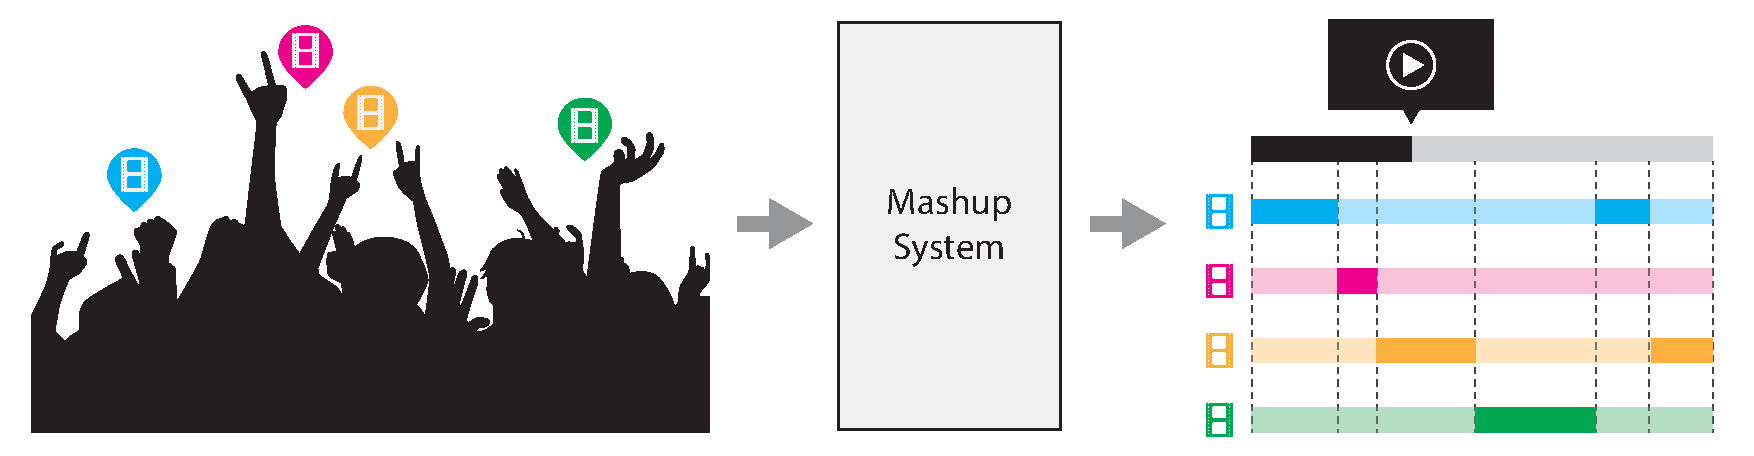
\includegraphics[clip=true, width=0.95\textwidth]{mashup-illustrate.pdf}
    \caption{移动多摄像头视频自动剪辑示意图}
    \label{fig:mashup-illustrate}
    \vspace{-2em}
\end{figure}

然而,移动多摄像头视频自动剪辑面临着一些困难。第一个困难来自于移动视频的质量。虽然拍摄设备
已经获得了巨大的发展和提升,视频质量依然会受到抖动、模糊以及拍摄过程中其它因素的影响。
此外,音频质量还受到周围环境以及麦克风本身的影响。据我们所知,
目前很少有关于非侵入式(non-intrusive)音频质量评估的研究。
另一个困难在于无法公式化地描述专业编辑人员剪辑视频的过程。不同的编辑人员有不同的
编辑风格,很难学习通用的模型用于视频剪辑。即使对人工视频剪辑过程有了详细的了解,
仍然需要将剪辑的过程转化成可计算的表达和算法,
这个转化过程也是克服多摄像头视频剪辑两个基本问题的关键:
何时应当从一个音/视频源切换到另一个音/视频源?切换时如何选择最佳的音/视频源?

\section{可计算视频剪辑语法}
移动视频自动剪辑和电影剪辑密切相关。电影剪辑人员运用专业的剪辑语法,
通过影片的时间片段、阴影效果以及声音抓住用户的注意力,调动用户情绪,
向用户讲述电影所要传达的故事。电影剪辑语法是指用来表述
视觉形式、声音组合、它们存在和出现的功能以及播放时的相互关系的一套理论。
因此,电影剪辑语法包含运动、声音、图像、颜色、电影符号、编辑、蒙太奇等元素~\cite{manchel1990film}。
电影语法最基本的元素包括镜头、运动和距离(全景,中景,近景)~\cite{CinemaElements1982}。
不同的镜头长度、拍摄角度以及距离远近可以传达不同的观感。例如,局部的物体运动
可以通过中景镜头表达,而近景通常用来表达静态镜头或者缓慢运动的镜头。

移动视频自动剪辑模仿电影剪辑的过程来传达原始多摄像头视频记录的事件。移动多摄像头视频自动剪辑中,
切换点是指镜头之间的边界时间点,镜头选取是指选取合适的视频流。为了创建内容丰富、剪辑专业的视频,
首先需要了解电影剪辑语法以及剪辑人员如何运用这些语法到实际的剪辑中。

运用电影剪辑的一个主要难点在于电影剪辑并不是严格的准则。
虽然已经有大量的工作讨论电影语法,本文的部分的结论也不是新的发现,
总结已有的电影编辑规则,发掘新的与移动多摄像头视频剪辑相关的、并且方便转化成
可计算规则的电影语法仍然十分必要,这也是本章系统的基础。我们查阅了已有的
关于视频编辑的用户调研和论文,并进一步组织了关于视频剪辑两个基本问题的用户调研:
\begin{itemize}\setlength{\itemsep}{0pt}
    \item \textbf{镜头/录音切换}:何时该切换到另一个音频/视频源?
    \item \textbf{镜头/录音选取}:切换时如何选择将要切换到的音频/视频源?
\end{itemize}

\subsection{用户调研}
我们邀请了一位艺术设计领域的教授和一名电影摄影专业的研究生参与了用户调研。
该教授有20多年的视频相关领域的研究和从业经验,该研究生有着丰富的视频编辑经验尤其是和电视台的长期合作经验。

用户调研以讨论的形式进行。我们首先展示了典型的拍摄场景(如演唱会、比赛),移动多摄像头
视频的主要问题(光照、抖动、遮挡等等)。我们向他们解释移动多摄像头视频剪辑的含义并
咨询与之相关的问题。这些问题包括:
\begin{itemize}\setlength{\itemsep}{0pt}
    \item \emph{视频剪辑讨论}:该讨论主要调研切换频率和镜头选取。咨询的问题包括:
        视频镜头的时长是否有要求?哪些因素会影响到镜头时长?它们是如何影响的?
        这些因素与时长之间是否有确定的联系?镜头切换有哪些要求?
        哪些因素跟视频质量密切相关?如何避免移动多摄像头视频的单一性问题?
        如何能够平滑地切换视频镜头?是否有提高观看
        体验的建议?
    \item \emph{音频剪辑讨论}:该讨论主要是关于音频的选取,问题包括:何时需要从一个
        音频源切换到另一个音频源?什么样的音频是比较好的?视频剪辑和音频剪辑之间的差异
        是什么?不同音频源的片段之间如何拼接?
\end{itemize}

\subsection{视频剪辑调研结果}
\label{sec:video-mashup-survey}
\textbf{镜头切换}。两个编辑人员认为视频镜头的时长应该有个范围,
太短的镜头内容表达不完整,太长的镜头则显得枯燥。镜头时长不是一个固定的常数值。
Shrestha等人选取的演唱会视频镜头的长度为3秒到7秒~\cite{shresthabws10}。然而,镜头时长也不是严格固定的,
更长的镜头可以用于运动镜头或者定场镜头,因为运动镜头不断拍摄新的内容,防止了内容的
枯燥性,而定场镜头展示了完整的场景和丰富的内容,也不会导致内容单一引起的枯燥性。

镜头切换的频率跟音频和视频都比较相关。较高的切换频率适用于较快的音频节奏,剧烈的物体运动、
以及快速的光照变化,平缓的镜头适宜配以较少的镜头切换。镜头切换频率和这些影响因素之间没有
明确的关系,采用线性关系或者非线性关系取决于编辑者的编辑风格。

合适的切换点应该选择在说话或者歌唱的间歇。开始说话或者唱歌能够抓住观看者的注意力,
并在结束时释放。为了避免打断观看者的注意力,在说话或者唱歌的间歇切换通常是比较好的选择。

\textbf{镜头选取}。与镜头选取相关的可计算的因素包括:视频质量、多样性、相机运动和语义
完整性。
\begin{itemize}\setlength{\itemsep}{-0.5em}
    \item \emph{视频质量}。视频质量保证了视频的清晰度和观看体验的愉悦性。有关视频质量的发现
        包括:太暗或者太亮的镜头应该被排除;应避免模糊的镜头;遮挡的镜头会破坏用户兴趣;
        倾斜镜头多数情况下会让观看者感到不适,虽然特殊情况下能够达到特殊的表达效果。
        两位参与者还特别提到由不规律或者不专业的相机运动引起负面效果(如手的抖动、快速运动等)
        的镜头必须排除。
    \item \emph{多样性}。多样性表示对事件丰富的内容表达。根据调研,
        视频剪辑中没有明确的准则用来选择相机的角度和距离。
        不同的剪辑人员有不同的剪辑风格,因而在有多个镜头可选时可能也会做出不同的选择。
        然而,镜头选取中也有一些不能违反的规则。比如,一个关键的准则是避免\emph{跳切}:
        拍摄相同主体的两个相邻镜头的拍摄位置和角度不能过于接近。\emph{30度准则}表明相邻镜头
        至少应该有30度拍摄角度的差异,从而避免镜头内容大量的重合。
        当相机位置不确定时,剪辑人员推荐应当选择镜头使得帧与帧之间的差别足够大,给观看者
        呈现新的内容。
    \item \emph{相机运动}。为了良好的观看体验,相邻镜头的相机运动应该尽量平滑,
        意外的相机运动会导致令人厌烦的视觉影响。一些通用的准则包括:(1)静态镜头应该与
        静态镜头连接;(2)运动镜头不适宜放置一起;(3)可以通过减慢的相机运动消除运动镜头和
        静态镜头连接导致的部分视觉影响。
    \item \emph{语义完整性}。两位参与者提到视频剪辑语义上的一些考虑。
        每个用户拍摄的视频都是由一系列语义完整的部分(后文中我们称之为子镜头)构成。
        视频剪辑不应该破坏每个部分的语义完整性,切换时应该选取语义完整的镜头,
        否则镜头切换会显得十分突兀。
\end{itemize}

\subsection{音频剪辑调研结果}
不同与视频剪辑,音频切换的次数应该越少越好,我们称之为\emph{最小切换准则}。在音频剪辑中
不存在一直播放同一音频源导致的单一性问题。相反,即使多个视频之间在时间上精确同步,
由于音频音量音色的差异,连接不同的音频源会导致不连贯的问题。这种不连贯性既有可能是
麦克风本身也有可能是录音时的周围环境引起的,使得剪辑音频质量下降。因此,音频剪辑更倾向
于从一个或少数几个音频源创建单一音频流。考虑到移动拍摄环境,应该避免嘈杂的音频,选择
声音清晰干净的音频片段,音频剪辑应该具有鉴别高质量音频片段的能力。

\subsection{可计算视频剪辑语法}
根据用户调研,我们对可计算的视频剪辑语法做了总结。这些语法构成了本章节提出的系统的基础。
\begin{itemize}\setlength{\itemsep}{-0.4em}
    \item 对于视频切换点检测,需要满足以下条件:(1)镜头时长应该在一个范围之内;
        (2)镜头切换的频率应该与音频的节奏相匹配;
        (3)切换点应该选择在说话或者唱歌的间歇。
    \item 视频镜头选取应该满足以下准则:(1)镜头应该清晰稳定(没有模糊、遮挡、抖动等
        问题); (2)相邻镜头之间的帧差应该较大, 避免\emph{跳切};(3)切换点附近的
        相机运动应该平滑自然;(4)每个被选择的镜头语义上应该完整。
    \item 音频剪辑应该满足:(1)音频片段清晰干净;(2)满足\emph{最少切换准则}:音频
        切换的次数应该越少越好。
\end{itemize}

\section{移动多摄像头视频自动剪辑系统}
基于以上总结的可计算视频剪辑语法,本节提出MoVieUp系统用于解决移动多摄像头视频
自动剪辑问题。后续章节中,视频和音频分别表示视觉信号和音频信号,用录像同时表示两个信号。

\begin{figure}[t]
    \centering
    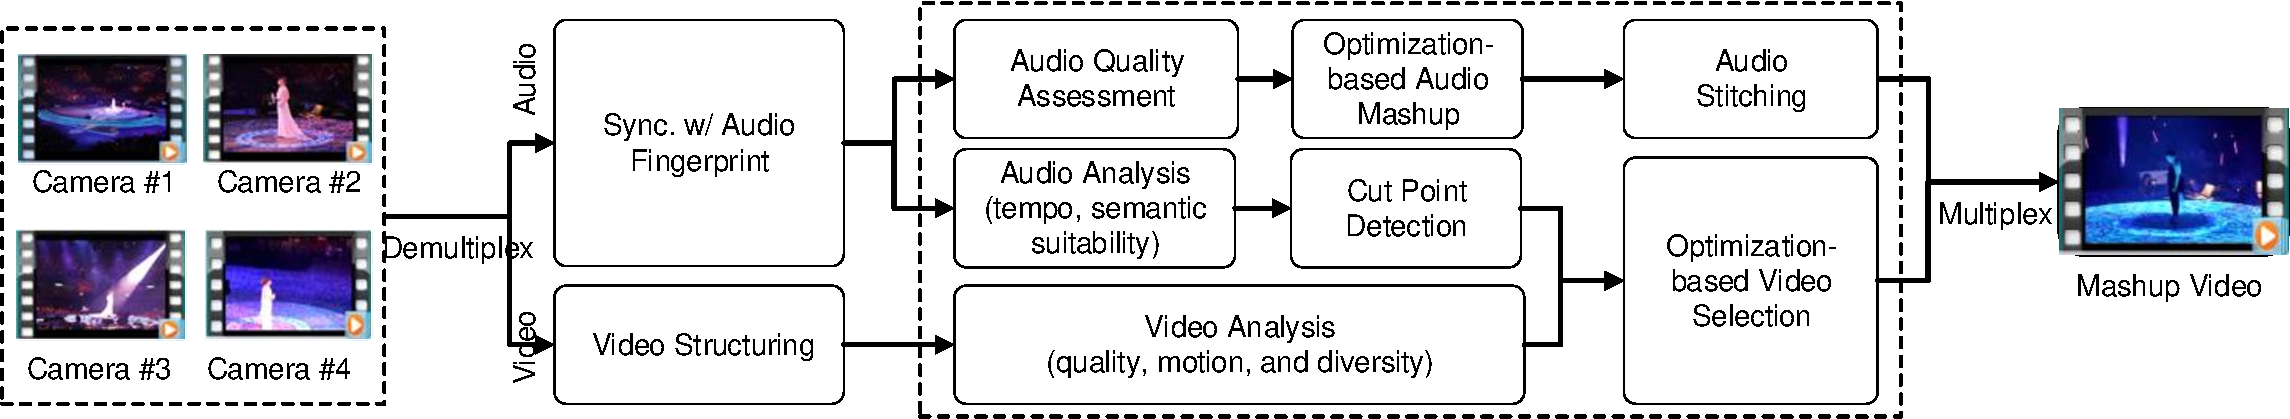
\includegraphics[clip=true, width=0.98\textwidth]{mashup-framework.pdf}
    \caption{移动多摄像头视频自动剪辑系统框架}
    \label{fig:mashup-framework}
    \vspace{-2em}
\end{figure}

\subsection{系统框架}
MoVieUp系统包含音频剪辑和视频剪辑两个部分。为了更清晰地阐述系统原理,定义以下术语:
\vspace{-0.5em}
\begin{itemize}\setlength{\itemsep}{-0.5em}
    \item \emph{子镜头}:包含连续相机运动和独立语义内容的基本视频单元。
    \item \emph{镜头}:剪辑后的视频中来自于同一个视频源的连续子镜头。
    \item \emph{切换点}:从一个信号源切换到另一个信号源的时间点。需要注意的是,
        在每个切换点,可能有多个信号源作为选择。
\end{itemize}

图~\ref{fig:mashup-framework}显示了MoVieUp系统的框架。
给定一组录像,系统将它们分流成音频和视频、在时间上对录像同步、
根据可计算的视频剪辑语法生成剪辑后的音频和剪辑后的视频,并混流成最终的单一音视频流。
对于音频剪辑,系统在\emph{最少切换准则下}根据音频质量选择音频片段。
视频剪辑包含两个步骤:切换点检测和视频镜头选取。系统通过匹配切换频率和音频节奏
并在说话或唱歌的间歇检测切换点。给定检测到的切换点,镜头选取在保证相机运动一致性
的条件下最大化视频质量和多样性。质量和内容的分析在子镜头的粒度上完成。
系统对视频剪辑的结果进一步微调,从而满足语义完整性。
视频抖动矫正作为可选的步骤可以进一步提高剪辑视频的观看体验。
系统完成音频剪辑和视频剪辑以后,对两个剪辑结果混流生成最终的结果。

\textbf{符号表示}:假设一共有$N$个录像$\mathcal{R}=\{r_1, r_2, \ldots, r_N\}$。
每个录像$r_i$被分流成音频$a_i$和视频$v_i$。$r_i$开始的时间记为$t_i^{(s)}$,结束的时间记为
$t_i^{(e)}$,$a_i$和$v_i$开始和结束的时间与$r_i$相同。第$j$个被选取的音频和视频片段表示为
$s_j^a$和$s_j^v$(第$j$个镜头),相应的时长表示为$d(s_j^a)$和$d(s_j^v)$。
上标$a$和$v$用来区分音频和视频。剪辑后的音频和视频表示为:
\begin{eqnarray*}
    \mathcal{M}^a &= (s_1^a, s_2^a,\ldots, s_{M^a}^a) \\
    \mathcal{M}^v &= (s_1^v, s_2^v,\ldots, s_{M^v}^v).
\end{eqnarray*}

对于视频剪辑,每个镜头最大时长为$d_{max}$,最小时长为$d_{min}$:$d_{min} \leq
d(s_j^v) \leq d_{max}$。切换点$c_j$是视频从$s_{j-1}^v$切换到$s_j^v$的时间点,
对应的时间记为$t_{c_j}^v$。为了表示方便,事件开始的时间也认为是一个切换点,即
$t_{c_1} = 0$。图~\ref{fig:mashup-symbols}表示了以上符号的含义。
\begin{figure}[t]
    \centering
    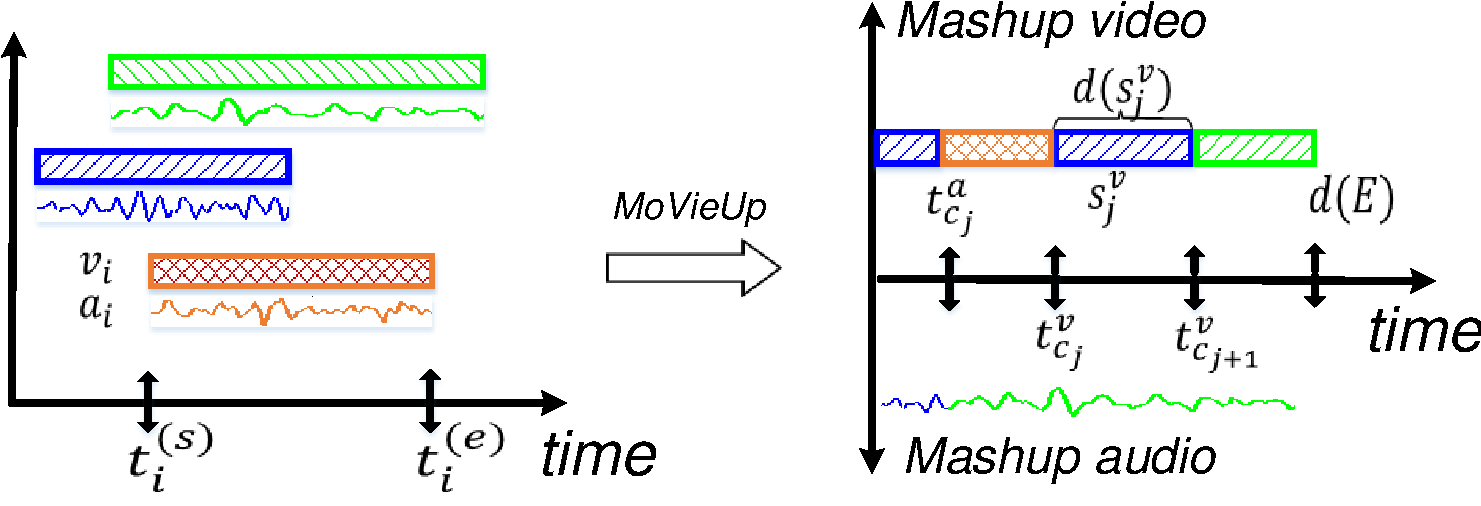
\includegraphics[clip=true, width=0.95\textwidth]{mashup-symbols.pdf}
    \caption{移动多摄像头视频自动剪辑系统符号表示}
    \label{fig:mashup-symbols}
\end{figure}

\textbf{预处理}:系统首先对音视频做预处理,方便后续的分析和优化。
音频被采样到8kHz,视频帧率被采样到25帧/秒,分辨率被采样到$640\times 360$。

输入的一组录像记录了同一事件的不同时间段。为了进一步的处理,需要将录像在时间上同步,
确定每个录像的起止时间$t_i^{(s)}$和$t_i^{(e)},\forall r_i \in \mathcal{R}$。
同步的基本假设是在事件的任意时间点至少存在一个录像。MoVieUp采用了
Shrestha等人提出的基于音频指纹的方法对录像同步~\cite{shresthabws10}。
系统首先提取每个录像的音频指纹,通过比较计算出每一对录像之间的时间差,
再通过投票的方法决定所有录像之间的时间差。

视频和音频剪辑都需要满足同步约束:被选取的信号源的开始时间必须早于当前切换点,
结束时间必须晚于当前切换点。
\begin{eqnarray}
    t_{s_j}^{(s)} \leq t_{c_j} \leq t_{c_{j+1}} \leq t_{s_j}^{(e)}
\end{eqnarray}
当不满足上述约束时,对应的信号源将不作为当前切换点的备选信号源。

对于视频的处理有三个粒度:帧,子镜头和镜头。如同Mei等人的分析~\cite{MeiHZZL07},
帧并不是视频最具有信息量的语义单元,帧级别的操作不仅十分耗时,
也不利于进一步的内容分析。镜头是由于用户开始和结束操作引起的物理结构,
持续的时间相对较长,包含的内容不一定具有一致性。
本章剪辑系统选取了包含连续相机运动和完备语义内容的
子镜头作为基本视频单元,并采用Kim等人提出的基于颜色和运动阈值的方法对输入视频
做结构分析,得到视频的子镜头~\cite{KimCKK00}。

\subsection{音频剪辑}
在多摄像头视频剪辑中,每个录音只记录了整个事件一段时间,
音频剪辑是把所有录音综合起来生成事件的单一的完整的音频的过程。本章系统
在\emph{最少切换准则}下最大化音频质量剪辑音频。

根据用户调研的结果,音频剪辑的主要目的是最大化选取的音频片段的
整体质量$Q(\mathcal{M}^a)$。由于音频切换会降低最终生成音频的质量,
$Q(\mathcal{M}^a)$并不是简单的各个音频片段的质量之和。
通过仔细研究,我们发现每个移动设备拍摄的音频质量并不会频繁剧烈的抖动。
基于这个发现,我们将\emph{最小切换准则}具体化为一个音频切换的硬性约束。
用$q_{s_j^a}(t)$表示音频片段$s_j^a$在时间$t$的质量,
仅当其它音频的质量明显好于当前音频时才发生切换:
\begin{eqnarray}
    q_{s_{j+1}^a}{(t)} & > \gamma \cdot q_{s_j^a}{(t)},
    \label{equ:mashup-switch-constraint}
\end{eqnarray}
$\gamma$是音频切换的惩罚系数,在实验中设为$1.2$。

系统采用贪心算法每隔一秒检查所有备选音频的质量,生成最终的剪辑音频。
音频切换发生在当前音频结束时或另一个音频的质量明显好于当前音频时。

\textbf{音频质量评估}:上述方案需要评估音频的质量。据了解,
除了一些在语音信号上的工作~\cite{CampbellJG09},很少有无参考的通用音频质量评估的解决方案。
Li等人将无参考音频质量评估建模为排序学习问题~\cite{LiWCDWW13},
该工作也是通用音乐质量评估的第一个工作。然而该方法并不适用于本章的音频剪辑场景,
如方程~\eqref{equ:mashup-switch-constraint}所示,音频剪辑需要有意义的音频质量评分。

通常,移动多摄像头视频拍摄的事件中音频信号的主体是说话或者歌唱。
因此本章系统采用了P.563~\cite{RixBKKG06}——一种非侵入式语音质量评估算法
评价输入音频的质量。系统用5秒滑动时间窗评价每秒的音频质量。

为了验证P.563算法是否适用于移动多摄像头视频的音频质量评估,我们随机选取了
四个移动设备录制的音乐会录音,并下载了对应的音乐,称之为参考音频。
我们用P.563算法分别评价这两种类型的音频质量,质量分数如图~\ref{fig:mashup-audio-example}所示。
图中横轴是时间,纵轴是质量评分(Mean Opinion Score, MOS)。
左图中是四个移动音频的质量评估结果,右图中是对应的参考音频质量评估结果。
可以发现移动音频的质量评分明显低于参考音频的评分,验证了P.563
算法在移动多摄像头视频场景下的有效性。音频剪辑的目标是选取图~\ref{fig:mashup-audio-example}
所示的Audio 2开始阶段持续时间长的高质量音频片段。
\begin{figure}[t]
    \centering
    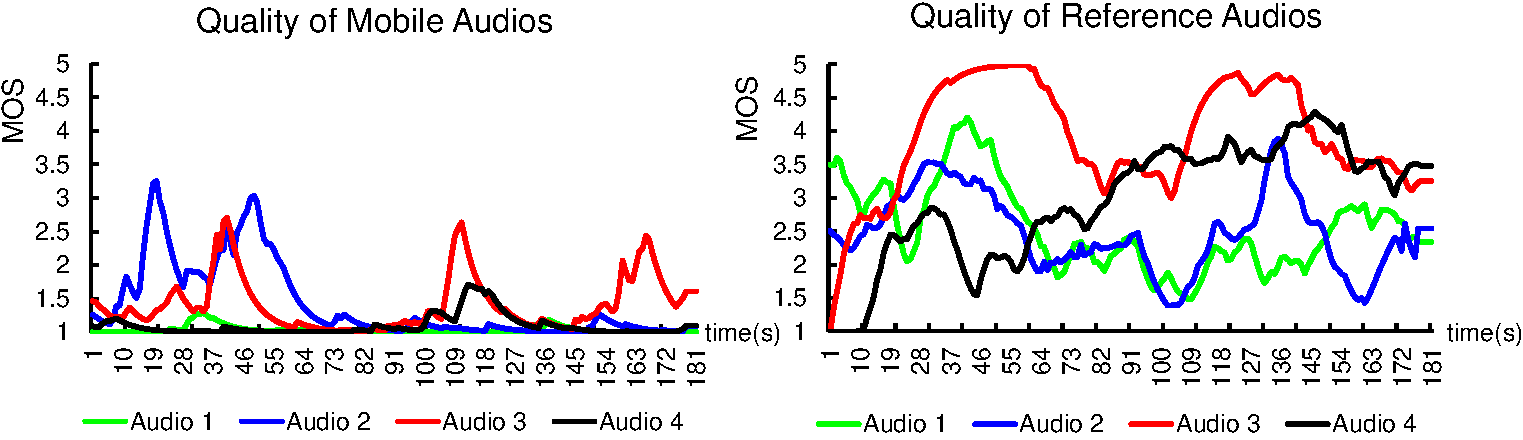
\includegraphics[clip=true, width=0.95\textwidth]{mashup-audio-example.pdf}
    \caption{音频质量评估结果示例}
    \label{fig:mashup-audio-example}
\end{figure}

\textbf{音频拼接}:选取音频片段以后,系统需要将音频片段拼接成单一音频。
不同于视频镜头可以直接拼接,用户对声音的突然变化比较敏感。由于输入的录音是由不同设备
在不同位置不同周围环境下录制的,直接拼接音频片段会导致音量和音色不一致引起的声音突变问题。
为了克服这个问题,系统首先用直流矫正使得音频的音量增益相同,并使用类似与图片融合的基于
拉普拉斯金字塔的算法将音频片段拼接成单一音频。

\subsection{镜头切换点检测}
\label{sec:mashup-cutpoint}
视频剪辑是从输入视频中选取镜头并将它们拼接成内容丰富、具有专业观赏品质的单一视频流。
视频剪辑分为两个步骤:切换点检测和视频镜头选取。本节介绍切换点检测,
研究视频剪辑应该何时从一个视频源切换到另一个视频源。

根据可计算的视频剪辑语法,视频切换点检测需要综合考虑音频(音频节奏、说话/歌唱间隔)
和视频(相机运动、子镜头完整性等)。MoVieUp系统首先根据剪辑后的音频检测备选的切换点。
对于视频,系统要求在备选的切换点处选取镜头时需要满足运动一致性和语义完整性。
我们提出了两个合适度用于检测视频切换点:节奏合适度$S^T(t)$和语义合适度$S^S(t)$。
节奏合适度衡量切换频率和音频节奏之间的关系,语义合适度避免打断说话或歌唱等行为。
切换点检测假设当前检测点以前的切换点已经被确定,用数学形式表达为:
\begin{equation}
    \begin{aligned}
        t_{c_j} = \argmin_{t}&\big\{{S^T(t|t_{c_{j-1}}) +
        S^S(t|t_{c_{j-1}})}\big\}, \quad s.t. \quad
        d_{min} &\leq t - t_{c_{j-1}} \leq d_{max}
    \end{aligned}
    \label{equ:mashup-cut-pint-detection}
\end{equation}

\textbf{节奏合适度$S^T(t|t_{c_{j-1}})$}:视频切换频率应该与音频节奏匹配。快节奏的音频
应该配以频繁的镜头切换,低频镜头切换更适合用在节奏缓慢的事件中。我们用音频起始点(onset)
之间的间隔近似音频节奏~\cite{DBLP:conf/mm/HuaLZ03,stowell2007adaptive}。
如同在~\ref{sec:video-mashup-survey}节讨论的,音频节奏和切换频率之间没有明确的关系。我们将时刻$t$的节奏$b(t)$
线性地映射到预期时长$d(b(t))$:
\begin{equation}
    d(b(t)) = d_{max} - \frac{d_{max} - d_{min}}{b_{max} - b_{min}} (b(t) - b_{min}),
\end{equation}
其中$b_{max}$和$b_{min}$分别是最大和最小音频节奏。

$t$时刻的节奏合适度定义为:
\begin{equation}
    S^T(t|t_{c_{j-1}}) = |\int_{t_{c_{j-1}}}^{t}{\frac{1}{d(b(t))}dt} - 1|.
\end{equation}

\textbf{语义合适度$S^S(t|t_{c_{j-1}})$}:语义合适度$S^S(t)$表示应该避免让镜头切换
分散用户的注意力。系统通过选择音频能量较低的时间点(如说话/歌唱间隔)
作为切换点达到这个目的。语义合适度通过归一化到$[0,1]$范围内的音频能量$e(t)$衡量:
\begin{equation}
    S^S(t) = e(t).
\end{equation}

\textbf{切换点检测}:目标方程~\eqref{equ:mashup-cut-pint-detection}是一个连续函数,由于
节奏合适度和语义合适度都不是平滑函数,很难求出该目标方程的闭合解。因此,我们将时间
离散化,离散化步长为$\delta$秒,系统枚举从上一个切换点开始的$[d_{min},d_{max}]$范围内的
所有可能时间点,目标方程的求解转化为:
\begin{equation}
    \begin{aligned}
        t_{c_j}   &= t_{c_{j-1}} + K\delta, \\
        where \quad K &= \argmin_{K}\big\{S^T(K) + S^S(K)\big\},\\
        S^T(K)  &= \big|\sum_{k=1}^K{\frac{\delta}{d(b(k))}} - 1\big|, \\
        S^S(K)  &= e(K)= e(t_{c_{j-1}^v}  + K\delta), \\
        b(k)    &= b(t_{c_{j-1}^v}  + k\delta).\\
    \end{aligned}
\end{equation}

在理想情况下,$\delta$的值应该尽可能小,从而逼近连续的目标方程。
为了选取合适的$\delta$值,我们随机选取了一些音频并用不同的$\delta$值检测切换点。
图~\ref{fig:mashup-cut-point}显示了在两个随机选取的音频上检测切换点的结果,
横轴为切换点的序号,纵轴为对应的时间点。
我们发现当$\delta$小于$0.2$秒时,检测到的切换点十分类似。因此,我们在实验中$\delta$
取值为$0.1$。用$d(e)$表示事件的时长,当$d(e)$在几分钟的量级时,
目标方程~\eqref{equ:mashup-cut-pint-detection}需要枚举的时间点个数为$d(e)/\delta$,
一般不超过几千个检测点的量级,相应的计算复杂度也在合理的范围内。
\begin{figure}[t]
    \centering
    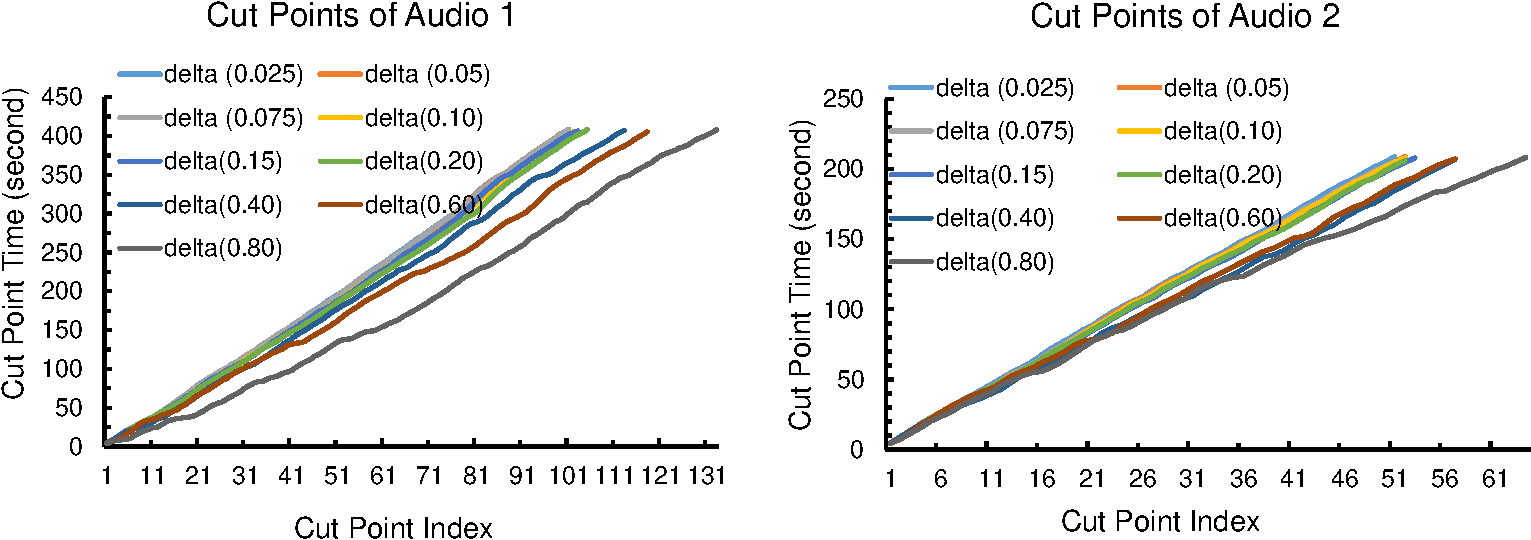
\includegraphics[clip=true, width=0.95\textwidth]{mashup-cut-point.pdf}
    \caption{不同$\delta$取值对视频切换点检测的影响}
    \label{fig:mashup-cut-point}
\end{figure}

\subsection{视频镜头选取}
视频镜头选取是在每个切换点确定如何选取应该切换到的视频源。
本节将视频镜头选取建模为相机运动一致约束下的优化问题。

根据用户调研的结果,视频镜头选取需要综合考虑视频质量、多样性、相机运动和语义
完整性。由于语义完整性依赖被选取的镜头,我们将会在后处理中考虑语义完整性。
因此,视频镜头选取建模为相机运动一致性约束下最大化视频质量和多样性问题。
具体来说,为了简化相机运动一致性的约束,我们禁止选取在切换点有相机运动的镜头。
该简化方案能达到两个效果:(1)减小连接运动镜头带来的视觉冲击;(2)平滑相机运动的变化,
避免打断相机运动。

用$\m^-(s_j^v)$和$\m^+(s_j^v)$表示第$j$个被选取的镜头$s_j^v$左右两边的相机运动,
相机运动一致性表示为:
\begin{equation}
    \m^-(s_j^v) = \m^+(s_{j}^v) = 0,
\end{equation}

用$Q(\mathcal{M}^v)$表示剪辑视频的质量,$D(\mathcal{M}^v)$表示多样性,视频镜头选取
定义为:
\begin{equation}
    \begin{aligned}
        \mathcal{M}^v = \argmax_{(s_1^v, \ldots, s_{M^v}^v)}\big\{Q(\mathcal{M}^v)& + D(\mathcal{M}^v)\big\}, \quad s.t. \\
        \m^-(s_j^v) = \m^+(s_{j - 1}^v) &= 0, \forall j \in [2,M^v].
    \end{aligned}
    \label{equ:mashup-formu-vss}
\end{equation}

\textbf{视频质量评估}:不同与音频剪辑,视频质量不会因为镜头切换而降低。
视频剪辑的整体质量表示为:
\begin{equation}
    Q(\mathcal{M}^v) = \sum_{j=1}^{M^v}{Q(s_j^v)},
\end{equation}
其中$Q(s_j^v)$是时间段$[t_{c_j},t_{c_{j+1}}]$内镜头$s_j^v$的质量分数。

MoVieUp采用了无参考的视频质量评估方法衡量移动视频的质量。视频质量从两大类别(时间和空间)
六个方面进行衡量~\cite{MeiHZZL07}。时间因素,包括不稳定性(unstableness)和急动(jerkiness),
是由不规律的相机运动引起的。空间因素,包括失真(infidelity)、亮度(brightness)、
模糊(blurring) 和倾斜(tilting),是由于恶劣的拍摄环境引起的。系统在子镜头的粒度上
评估六个方面的分数$u_i^v \in [0,1], i \in [1,6]$。
子镜头的不合适分数$U$和质量分数$Q$通过两个步骤计算得到:
\vspace{-0.4em}
\begin{itemize}\setlength{\itemsep}{-0.4em}
    \item 预筛选低质量的子镜头。如果任一子镜头的某个质量分数低于对应的阈值,则认为
        该子镜头不适合被选取。系统将它的不合适度设为一个较大的值(在实验中设为$1,000$),
        从而保证在该子镜头持续时间内,仅有该子镜头可选时该子镜头仍会被选中。
    \item 基于准则的方法计算子镜头的整体不合适分数$U$和质量分数$Q$~\cite{MeiHZZL07}:
        \begin{eqnarray}
            &U &= E(u^v) + \frac{1}{10 + 6\gamma}\sum_{i=1}^6{(u_i^v -
            E(u^v))}, \nonumber \\
            &Q &= 1 - U.
        \end{eqnarray}
        其中$E(u^v)$是子镜头六个方面质量分数的平均值,$\gamma$是预先定义的常数值,用以调节
        $u_i^v$和$E(u^v)$之间的差异对整体分数的影响。
        按照Tao等人在论文中的设定~\cite{MeiHZZL07},$\gamma$取值为$0.20$。
        镜头质量$Q(s_j^v)$取所有子镜头质量的最小值。
\end{itemize}


\textbf{多样性}:整体多样性是所有选取镜头的多样性之和:
\begin{equation}
    D(\mathcal{M}^v) = \sum_{j=1}^{M^v}{D(s_j^v)},
\end{equation}
其中$D(s_j^v)$是选取的第$j$个镜头的多样性。多样性主要与用户观看过的仍停留在记忆中内容有关。
系统根据多大程度上镜头能唤起用户记忆中的内容来衡量多样性。$D(s_j^v)$的计算方式为:
\begin{equation}
    D(s_j^v) = D(s_j^v, s_{j-1}^v).
\end{equation}
类似于Sundaram等人提出的记忆模型~\cite{sundaram2002computable},
两个镜头之间的记忆和多样性通过对应的相邻两个子镜头$a$和$b$计算得到:
\begin{equation}
    \begin{aligned}
        R(a,b) &= s(a,b)\cdot f_a \cdot f_b \cdot (1- \frac{\Delta t}{T_m} ), \\
        D(a,b) &= 1 - R(a,b),
    \end{aligned}
\end{equation}
其中$T_m$是记忆大小。 $s(a,b)$是相邻两个子镜头之间的相似度,
在MoVieUp系统的实现中采用了传统低层次的特征表达和相似度度量方法SSIM~\cite{WangBSS04Tip}。
为了进一步加强相似性度量,还可以收集常见的物体和场景类别,并从社交多媒体数据中收集相关的弱标注数据,
利用本文提出的弱监督深度学习方法,学习这些类别和场景的深度识别网络,
并利用本文提出的特征选取算法选取最能体现视频帧语义的特征,获取更好的镜头相似度的计算。
$f_a$和$f_b$是子镜头长度相对于记忆大小$T_m$的比例。$\delta t$是两个子镜头的时长差。

\textbf{镜头选取}:为了求解目标方程~\eqref{equ:mashup-formu-vss},我们将约束条件表示成
指示函数$I(s_j^v)$,当约束条件满足时$I(s_j^v)$等于0,否则取一个很大的值作为惩罚项
(系统实现中取值为$1,000$),从而保证当且仅当该镜头为唯一选择时才会被选中。
目标方程被重新表示为:
\begin{equation}
    \mathcal{M}^v = \argmin_{(s_1^v, \ldots, s_{M^v}^v)}
    \bigg\{ \sum_{j=1}^{M^v}{\big\{U(s_j^v) + I(s_j^v)\big\}}
    +  \sum_{j=2}^{M^v}{R(s_j^v, s_{j-1}^v)} \bigg \}.
    \label{equ:mashup-reformu-vss}
\end{equation}

上述目标方程可以定义成递归的形式。用$f(s_m^v:s_n^v)$表示切换点$m$到$n$(不包括$m$)
的上述目标方程的最优值:
\begin{eqnarray}
    f(s_m^v:s_n^v) &=& \min_{(s_{m+1}^v, \ldots, s_{n}^v)}\bigg\{ R(s_{m}^v,
        s_{m + 1}^j) \nonumber \\
        &&+ \sum_{j=m + 1}^{n}{\Big( U(s_j^v) +I(s_j^v)\Big)}
    + \sum_{j = m + 2}^{n}{R(s_{j - 1}^v, s_{j}^v)} \bigg\}  \nonumber \\
    &=& \min_{s_{m+1}^v}\bigg\{U(s_{m+1}^v) + I(s_{m+1}^v)
        + R(s_{m}^v, s_{m + 1}^j)
    +f(s_{m+1}^v:s_n^v)\bigg\}, \nonumber \\
    where&& 1\leq m \leq n \leq M^v.
    \label{equ:mashup-recur-vss}
\end{eqnarray}

递归方程~\eqref{equ:mashup-recur-vss}具有最优子结构性质,为了优化$f(s_m^v:s_n^v)$,
首先需要针对每一个可能的$s_{m+1}^v$优化$f(s_{m+1}^v:s_n^v)$。利用最优子结构性质以及递归方程,系统通过动态规划获得最优解。

假设存在虚拟的唯一初始镜头$s_0^v$并满足所有约束条件。初始目标方程~\eqref{equ:mashup-reformu-vss}
可以利用动态规划和方程~\eqref{equ:mashup-recur-vss}求解得到。
\begin{eqnarray}
    \mathcal{M}^v = \argmin_{(s_1^v, \ldots,
    s_{M^v}^v)}{f(s_0^v:s_{M^v}^v)}, \nonumber\\
    U(s_0^v) = I(s_0^v) = 0, R(s_0^v, s_1^v) = 0.
    \label{equ:mashup-vss-final-obj}
\end{eqnarray}

\textbf{后处理}:根据用户调研的结果,每个录像都是由许多语义完整的子镜头构成的。
上述剪辑步骤没有考虑语义完整性。切换点可能出现在子镜头中间,使得被选取的子镜头太短,
破坏了语义完整性。此外,应该进一步减少不规则相机运动引起的抖动,提高用户体验。

因此,系统对剪辑结果进行两步后处理操作:语义完整性和视频抖动矫正。对于语义完整性,系统对切换点附近的
子镜头增加时长约束:如果某个子镜头持续的时间少于一秒,则对切换点的位置进行微调使得子镜头
的时长满足约束。对于视频稳定性,系统采用了Liu等人提出的视频抖动矫正方法减小移动视频抖动的影响~\cite{liu2013bundled}。


\vspace{-1em}
\section{实验结果和评估}
本节评价本章提出的移动多摄像头视频自动剪辑系统的效果。
图~\ref{fig:mashup-example}显示了移动多摄像头视频剪辑的一个样例。
时间轴上方是移动设备录制的备选音频,波形表示音频的能量曲线。
下方是移动设备拍摄的备选视频,视频通过每隔30秒采样的帧来表示。
系统从这些备选音频/视频中选取片段/镜头生成最终的剪辑音频/视频,
如图中绿色方框所示。
\begin{figure}[t]
    \centering
    \includegraphics[clip=true, width=0.95\textwidth]{mashup-example.pdf}
    \caption{移动多摄像头视频自动剪辑示例}
    \label{fig:mashup-example}
    \vspace{-2em}
\end{figure}

本实验从三个方面对系统进行评估:(1)音频剪辑是否提高了最终的音频质量。
实验与Virtual Director系统~\cite{DBLP:conf/mm/ShresthaWWBA10}进行对比,
该系统在选取视频镜头的同时选取对应的音频组成最终的音频输出;
(2)相比于人工选取的切换点以及Mukesh等人提出的基于学习的方法~\cite{DBLP:conf/mm/SainiGYO12},
本章提出的切换点检测算法效果如何?
(3)本章提出的MoVieUp自动剪辑系统是否提高了移动多摄像头的观看体验?
比较的基准包括两个现有系统:Virtual Director~\cite{DBLP:conf/mm/ShresthaWWBA10}和
Jiku Director~\cite{DBLP:conf/mm/SainiGYO12}。
评价主要从视频的质量、多样性、稳定性和整体的观看体验四个方面进行。

\subsection{数据集}
我们从Youtube网站\footnote{\url{http://www.youtube.com}}上收集了6个事件
一共46个录像,也是目前关于移动多摄像头视频自动剪辑最大的数据集。每个录像包含音频流和视频流。
所有录像都是由不专业的用户通过移动设备拍摄的。上述章节中提到的视频质量问题在数据集中普遍存在。
前三个事件的14个录像与Virtual Director使用的数据相同,
我们用Virtual Director的作者提供的剪辑视频\footnote{\url{http://www.youtube.com/AutomaticMashup}}作为比较对象。
剩下的32个录像被提交到Jiku Director中得到相应的剪辑视频。表格~\ref{tab:mashup-dataset-opt-time}
显示了数据集的详细情况。我们在一台8CPU 16GB
内存的Windows服务器上运行MoVieUp系统,平均需要45秒左右的时间评估一分钟
音频的质量。对于一分钟的视频,需要240秒左右的时间做视频结构化分析,65秒的时间做运动分析,
13秒的时间做质量评估。系统优化占用的时间如表~\ref{tab:mashup-dataset-opt-time}所示。

\begin{table}[htbp]
    \centering
    \caption{移动多摄像头视频数据集及算法优化时间}
    \label{tab:mashup-dataset-opt-time}
    \begin{tabular}{|c|c|c|c|c|c|c|}
        \hline
        事件 & 录像数目 & 时长 & 同步 & 音频剪辑 & 切换点检测 & 视频剪辑 \\
        \hline
        E1 & 5 & 4'37'' &1'44''  & 0.11'' & 1.58'' & 26.19''  \\ \hline
        E2 & 5 & 7'01'' &2'38''  &0.14'' & 2.26'' & 36.26''  \\ \hline
        E3 & 4 & 5'15'' &27''  &0.11'' & 1.90'' & 10.26''  \\ \hline
        E4 & 8 & 6'25'' &2'55''  & 0.10'' & 2.11'' & 2'49'' \\ \hline
        E5 & 11 & 3'32''&6'07''  & 0.11'' & 1.36'' & 6'26'' \\ \hline
        E6 & 27 & 5'22''&33'27''  & 0.19'' & 1.90'' & 19'24'' \\ \hline
    \end{tabular}
\end{table}

\vspace{-0.5em}
\subsection{实验设置}
音频剪辑评估采用用户调研的主观评估方法,评估遵循MOS评分策略:
1代表很差,2代表差,3代表一般,4代表好,5代表很好。
在用户调研中,我们给用户播放本章算法和Virtual Director产生的一对音频,
并要求用户给出评分。生成每个音频的系统对于用户是透明的,
每组音频的内部顺序对不同用户是随机的。

由于普通用户对于视频镜头切换点的敏感性比较低,很难对切换点的质量给出客观公正的评价。
为了更好地评价视频切换点,我们邀请了两位专业的视频编辑人员(与用户调研中的参与者不同)评价视频
切换点的合适度。同时我们也邀请两位编辑对切换点给出他们的意见。该评价围绕两个方面开展:
\vspace{-0.3em}
\begin{itemize}\setlength{\itemsep}{-0.3em}
    \item 切换频率是否合适?
    \item 切换点是否出现在合适的时机?
\end{itemize}

我们随机打乱了Virtual Director、Jiku Director和MoVieUp系统生成的一共12个剪辑视频的顺序。
两位专业人员需要依次观看这些视频并针对上面两个问题给出他们的评分,分数范围和含义与音频剪辑评估相同。

对于视频镜头选取,我们组织了在线用户调研比较不同系统产生的视频观看体验。
在调研开始前,我们提供了介绍页面帮助用户了解移动多摄像头视频自动剪辑以及用户
即将要完成的评价内容,包括多样性、视频质量、稳定性和总体评价四个方面,每个方面
的评价围绕以下问题展开:
\begin{itemize}\setlength{\itemsep}{-0.3em}
    \item \textbf{多样性}:视频是否给出了事件丰富的概览?该问题调查剪辑的视频
        内容是否有单一枯燥的问题。
    \item \textbf{视觉质量}:视频的视觉质量是否良好?
        此处的视觉质量主要是影响质量的空间因素。
    \item \textbf{稳定性}:视频是否稳定?由于抖动是移动视频的主要质量问题之一,
        我们单独评价视频的稳定性。
    \item \textbf{总体评价}:该视频剪辑是否专业?
\end{itemize}
我们要求用户针对每个视频回答上述四个问题并给出从1(完全不同意)到7(完全同意)的评分.

我们邀请了一位用户体验设计师设计了评价页面。不同于已有系统在实验中依次播放每个视频,
设计师建议我们同时播放两个对比视频,两个视频按图~\ref{fig:mashup-eval-interface}所示分左右
两边分别摆放。两个视频的顺序是随机的。用户在不知道视频顺序以及对应剪辑系统的情况下给两个视频分别打分。
这种评价方式的优点包括:
\vspace{-0.3em}
\begin{itemize}\setlength{\itemsep}{-0.3em}
    \item 用户可以直观地感受到两个视频之间的差异。在已有系统的实验中,
        用户需要记住对比视频的所有内容和细节。
    \item 同时观看两个视频不会让用户感到迷惑,
        如果同时播放更多的视频会分散用户的注意力。
\end{itemize}
根据以上设定,本章提出的MoVieUp系统在前三个事件上与Virtual Director比较,
在后三个事件上与Jiku Director比较。
\begin{figure}[t]
    \centering
    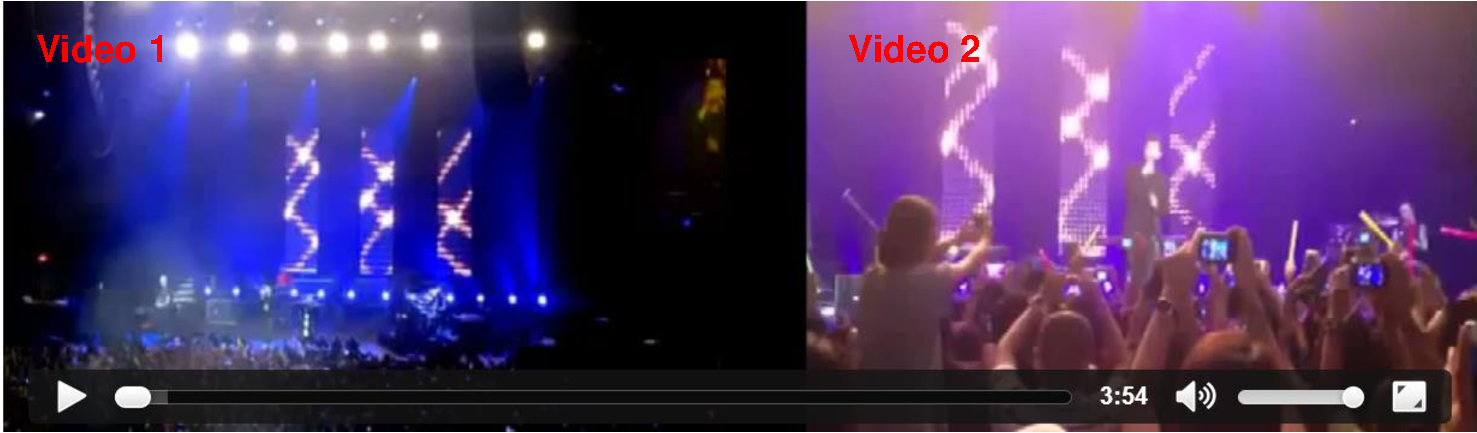
\includegraphics[clip=true, width=0.95\textwidth]{mashup-eval-interface.pdf}
    \caption{视频剪辑评价页面}
    \label{fig:mashup-eval-interface}
\end{figure}

\subsection{音频剪辑评价}
在音频剪辑评价中,我们进行了两组不同设置的实验。
第一组实验评价本章提出的音频拼接方式是否有效。由于
MoVieUp系统遵循\emph{最少切换准则},相应的音频剪辑的切换次数较少(如
表格~\ref{tab:mashup-audio-switch-times}所示)。
因此,实验从三个剪辑音频中选取了30秒切换最频繁的片段作为评价对象,
并与Virtual Director 产生的对应时间段的音频作比较。
\begin{table}[htpb]
    \centering
    \caption{音频剪辑切换次数比较}
    \label{tab:mashup-audio-switch-times}
    \begin{tabular}{|c|c|c|c|c|c|c|}
        \hline
        \multirow{2}{*}{系统} & \multicolumn{3}{c|}{设定1} &
        \multicolumn{3}{c|}{设定2}\\
        \cline{2-7}
        & 音频 1& 音频 2 & 音频 3 & 音频 4 & 音频 5 & 音频 6 \\
        \hline
        MoVieUp &\textbf{1} &\textbf{2} & \textbf{1} & \textbf{2} & \textbf{1}& \textbf{4} \\
        VD &5 & 5 & 4 & 86 & 23 & 76 \\
        \hline
    \end{tabular}
\end{table}

实验邀请了18名用户(包括14名男性和4名女性)参与用户调研。用户年龄在22岁到26岁之间。
其中,观看视频录像(演唱会、比赛等)的频率分布为:几乎不看--2人,每月--3人,
每周--6人,每天--7人。评价结果如表格~\ref{tab:mashup-audio-eval}所示。
本章提出的音频拼接方法可以有效减少音频切换带来的听觉影响,
尤其在音频的音量和音色差异较大时(音频2)时改善更加明显。
\begin{table}[htpb]
    \centering
    \caption{音频剪辑主观评价(MOS)比较}
    \label{tab:mashup-audio-eval}
    \begin{tabular}{|c|c|c|c|c|c|c|}
        \hline
        \multirow{2}{*}{系统} & \multicolumn{3}{c|}{设定1} &
        \multicolumn{3}{c|}{设定2}\\
        \cline{2-7}
        & 音频 1& 音频 2 & 音频 3 & 音频 4 & 音频 5 & 音频 6 \\
        \hline
        MoVieUp &\textbf{2.56} &\textbf{2.28} & \textbf{3.56} & \textbf{3.00} & \textbf{3.81}& \textbf{3.0} \\
        \emph{VD} &2.33 & 1.28 & 3.5 & 1.75 & 2.81 & 2.38 \\
        \hline
    \end{tabular}
\end{table}

第二组实验评价另外三个完整的剪辑音频。该设定的目的是检验本章提出的音频剪辑方法是否能够提高
音频剪辑的质量。我们邀请了另外16名用户参与用户调研,包括5名女性和11名男性,年龄分布从20岁到33岁。
观看视频录像的频率分布为:几乎不看--2人,每月--1人,
每周--10人,每天--3人。根据表格~\ref{tab:mashup-audio-eval}中设定2的结果可以发现,
MoVieUp系统的音频质量明显高于Virtual Director系统。

根据以上两个设定的实验结果,本章提出的系统从三个方面生成了更好的剪辑音频:
1)提出了更好的音频选取算法;2)显著减少了音频切换的次数;3)系统更平滑地
拼接各个音频片段,减少了音频切换引起的突兀的听觉效果。

\subsection{切换点检测评估}
本节比较本章提出的切换点检测算法相比于Virtual Director和Jiku Director
的效果,其中Virtual Director根据所有录像中质量最好的音频人工选取切换点,
Jiku Director和MoVieUp系统根据算法自动选取切换点。

\begin{figure}[ht]
    \centering
    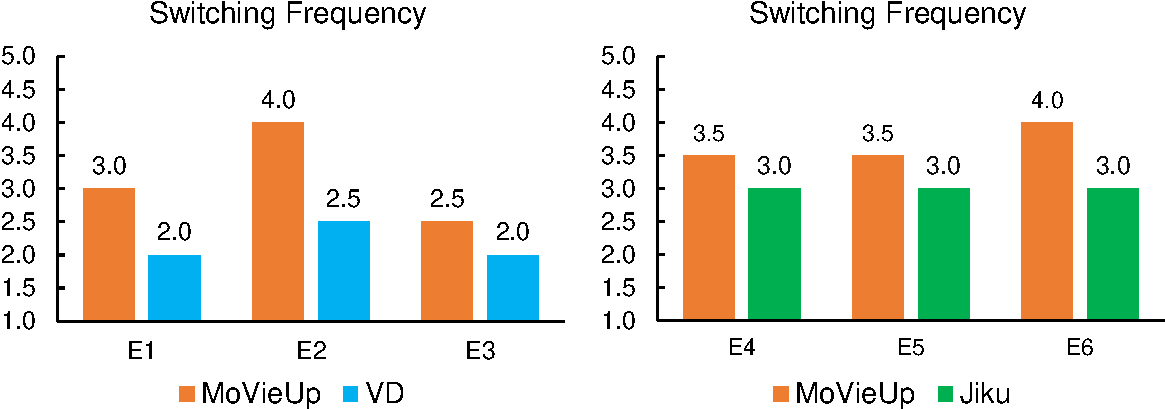
\includegraphics[clip=true, width=0.95\textwidth]{mashup-eval-switching-frequency.pdf}
    \caption{视频切换频率比较}
    \label{fig:mashup-eval-switching-frequency}
\end{figure}
图~\ref{fig:mashup-eval-switching-frequency}显示了关于切换频率的实验比较结果。
MoVieUp系统的切换点频率明显优于Virtual Director系统。考虑到Virtual Director系统
通过人工选取的方法获得切换点,我们与编辑人员讨论发现Virtual Director
选取了很多无意义的切换点。这些无意义的切换点是由于视频中出现了负面效果(抖动、遮挡等)引起的。
虽然我们的系统同样根据音频选取视频切换点,但它在视频质量方面的表现更好,避免了无意义的切换。
编辑人员提醒我们当没有合适的视频可供选取时,不切换通常是更好的选择。

\begin{figure}[ht]
    \centering
    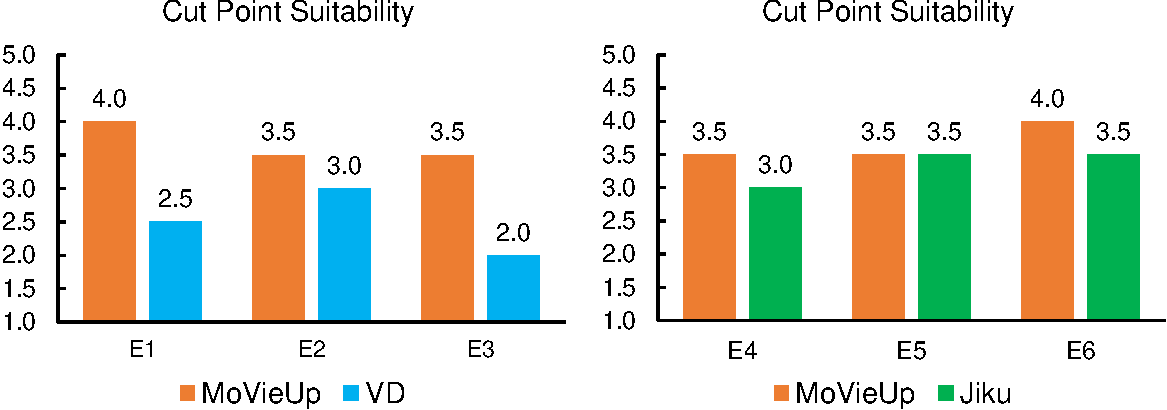
\includegraphics[clip=true, width=0.95\textwidth]{mashup-eval-cutpoint.pdf}
    \caption{视频切换点位置比较}
    \label{fig:mashup-eval-cutpoint}
\end{figure}
视频切换点位置合适度的比较结果如图~\ref{fig:mashup-eval-cutpoint}所示。
同样由于无意义的切换点,Virtual Director获得了很差的评分。
该结果验证了切换点检测不仅与音频有关,也依赖于视频信息。根据评分,MoVieUp
获得了比Jiku Director略好的结果。在用户调研中,
编辑人员推荐在说话或歌唱等语义行为的间隔切换,通过调研发现,部分文献建议在音乐的节奏点切换,
编辑人员也很难给出明确的切换点选取规则。即使如此,试验结果仍然表明MoVieUp提供了一个
可行的切换点检测方案,检测结果达到了\emph{一般}甚至\emph{好}的评价级别。

\subsection{视频剪辑评估}
本节从视频剪辑的角度评价MoVieUp系统相对于Virtual Director和Jiku Director
系统的观看体验。为了公平比较三个系统的表现,实验中MoVieUp系统没有采用视频稳定等后处理措施。

\textbf{与Virtual Director的比较}:
我们邀请参与音频剪辑第一组实验的18名用户参加MoVieUp系统与Virtual Director系统的比较实验,
比较结果如图~\ref{fig:mashup-comp-vd}所示。
\begin{figure}[ht]
    \centering
    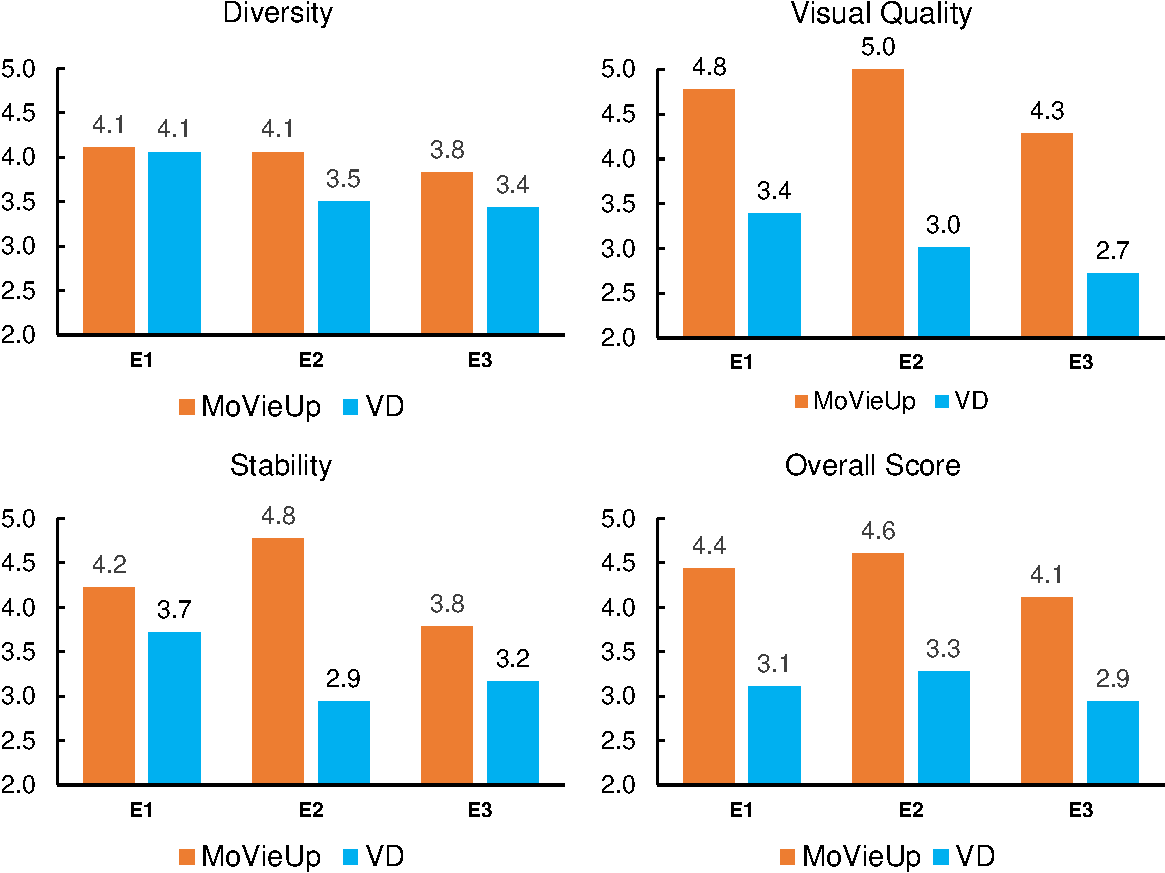
\includegraphics[clip=true, width=0.95\textwidth]{mashup-comp-vd.pdf}
    \caption{MoVieUp系统与Virtual Director系统视频剪辑结果比较}
    \label{fig:mashup-comp-vd}
    \vspace{-2em}
\end{figure}

通过比较发现,MoVieUp系统在多样性方面比Virtual Director系统表现更好,
但相对于其他三个评价因素,多样性的优势并不明显。该结果也在合理的范围之内,
因为两个系统都在切换点选取不同的视频源避免单调性问题,区别在于MoVieUp系统
考虑了时间因素,而Virtual Director系统仅依靠相邻两帧衡量多样性。此外,
我们分析了三个事件对应的视频,发现每个事件仅包含4到5个从不同角度和距离拍摄的视频,
视频源本身也能够避免一部分的单调性问题。

在视觉质量上,MoVieUp系统的表现更好。Virtual Director系统考虑了四个方面的
质量因素:块效应(blockiness)、模糊(blurriness)、亮度(brightness)和抖动(shakiness)。
MoVieUp系统考虑了更多的空间因素和时间因素,如倾斜(tilting)、失真(infidelity)和
急动(jerkiness)。质量预处理操作也滤除了质量很差的镜头。为了进一步研究系统表现好的原因,
我们邀请了三位专业的编辑人员从\emph{抖动}、\emph{过暗}和\emph{失真}
(包括由于遮挡和强光等原因引起的失真) 三个角度将剪辑视频的镜头标注成``好''或``差''。
\emph{倾斜}在本组视频中出现较少,模糊往往伴随\emph{抖动}出现,因而这两个因素没有单独标注。
标注的结果如表格~\ref{tab:mashup-vd-obj-comp}所示。在第一个事件中,
Virtual Director系统选取的46个镜头中有24个镜头存在过暗的问题(超过一半的画面是黑的)。
与之相应,MoVieUp系统选取的27个镜头中只有7个镜头存在过暗问题。
在第二个事件中,Virtual Director系统选取的55个镜头中有14个镜头受不规则相机运动的影响,
导致了\emph{抖动}问题,同样的问题在MoVieUp系统中只存在于两个镜头中。
我们对该事件的视频做了进一步的分析发现,5个视频中有4个视频存在抖动的问题。MoVieUp系统选取的2个抖动
镜头很可能是出于多样性的考虑。此外,失真也是影响视觉质量的关键因素。Virtual
Director系统选取了5个被强光污染的镜头,而MoVieUp系统中只有2个镜头有同样的问题。在第三个事件中,
Virtual Director系统选取的43个镜头中有8个存在抖动问题,MoVieUp系统只选取了1个抖动镜头。
根据实验结果和用户反馈,可以发现本章提出的系统可以从空间和时间两个方面选取出高质量的
视频镜头。
\begin{table}[t]
    \centering
    \caption{MoVieUp和Virtual Director系统存在质量问题的镜头数量比较}
    \label{tab:mashup-vd-obj-comp}
    \begin{tabular}{|c|c|c|c|c|c|c|}
        \hline
        \multirow{2}{*}{因素} & \multicolumn{3}{c|}{MoVieUp} & \multicolumn{3}{c|}{Virtual Director}  \\ \cline{2-7}
        & 事件1 & 事件2 & 事件3 & 事件1 & 事件2 & 事件3 \\ \hline
        镜头	& 27 & 27 & 29 & 46 & 55& 43 \\ \hline
        抖动	& 0 & 2 & 1 & 2 & 14& 8 \\ \hline
        过暗	& 7 & 0 & 0 & 24 & 1& 0 \\ \hline
        失真	& 0 & 2 & 5 & 0 & 5& 8 \\ \hline
    \end{tabular}
\end{table}

本章提出的MoVieUp系统在三个事件上从三个具体的方面都取得了比Virtual Director系统
更好的效果,验证了系统采用的多样性和视觉质量评估方法的有效性,同时也表明了系统采用的
算法可以获得在多样性和视觉质量上更优的结果和观看体验,也因此MoVieUp系统在整体评价上
获得了更高的评分。

\textbf{与Jiku Director的比较}:我们邀请了参与音频剪辑评估第二组实验的15名用户
参加与Jiku Director系统的比较实验。实验结果如图~\ref{fig:mashup-comp-jiku}所示。

\begin{figure}[ht]
    \centering
    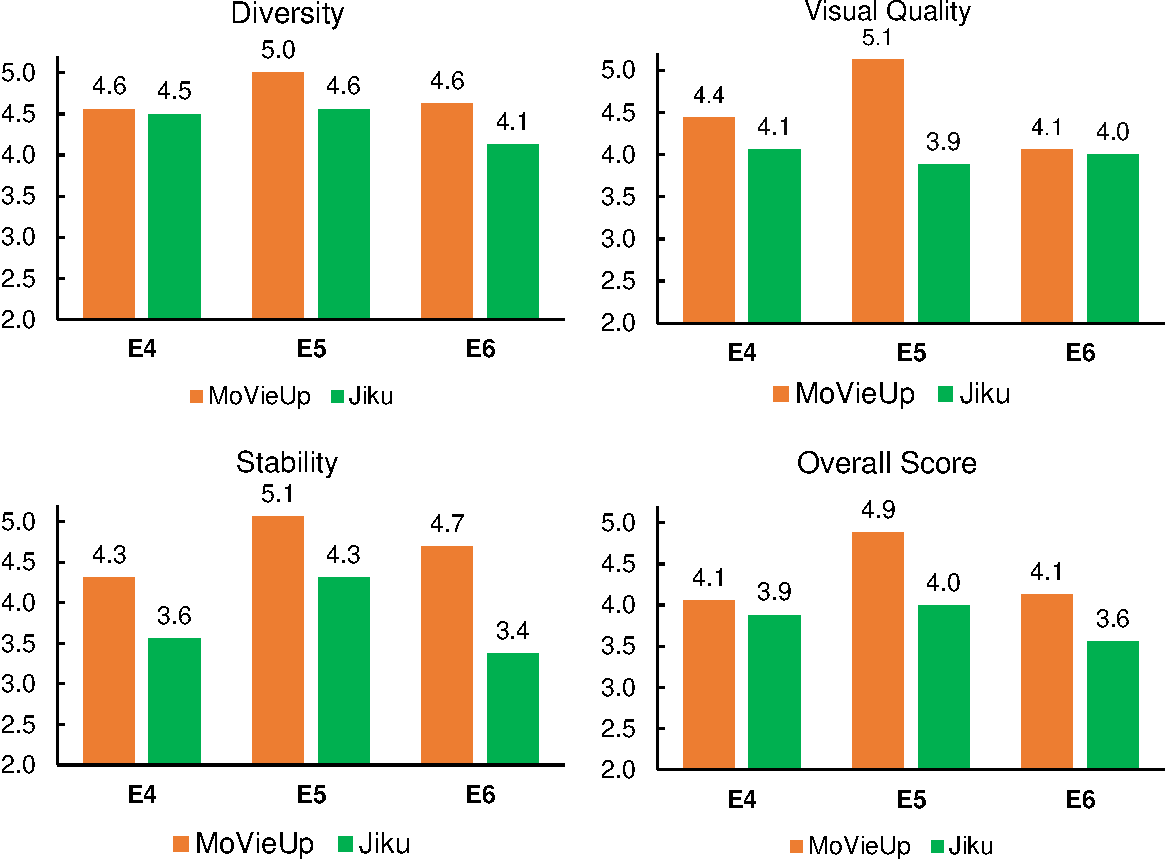
\includegraphics[clip=true, width=0.95\textwidth]{mashup-comp-jiku.pdf}
    \caption{MoVieUp系统与Jiku Director系统视频剪辑结果比较}
    \label{fig:mashup-comp-jiku}
    \vspace{-2em}
\end{figure}

\begin{table}[ht]
    \centering
    \caption{MoVieUp和Jiku Director系统存在质量问题的镜头数量比较}
    \label{tab:mashup-jiku-obj-comp}
    \begin{tabular}{|c|c|c|c|c|c|c|}
        \hline
        \multirow{2}{*}{因素} & \multicolumn{3}{c|}{MoVieUp} &
        \multicolumn{3}{c|}{Jiku Director}  \\ \cline{2-7}
        & 事件4 & 事件5 & 事件6 & 事件4 & 事件5 & 事件6 \\ \hline
        镜头		& 49 & 21 & 37 & 49 & 26& 49 \\ \hline
        抖动	& 3 & 0 & 0 & 11 & 3& 3 \\ \hline
        过暗	& 1 & 0 & 0 & 0 & 0& 1 \\ \hline
        失真	& 5 & 1 & 1 & 7 & 3& 4 \\ \hline
    \end{tabular}
\end{table}
多样性方面,MoVieUp系统获得了更好的效果,类似于与Virtual Director系统的比较结果,
多样性方面的提升并不明显。两个系统都采用了基于关键帧的相似度方法,都采用了用户对内容
的兴趣随着镜头时长递减的多样性模型。多样性方面的区别在于Jiku Director首先确定
镜头的视角(拍摄距离和角度),再从对应视角选取视频镜头。该策略可能在连续选取的视角比较接近
时的多样性较差,与之对比,MoVieUp系统基于记忆模型选取镜头。

视觉质量方面,两个系统在事件4和事件6上的表现比较接近。系统均考虑了空间和时间上的
质量因素。我们采用了与Virtual Director系统相同的客观比较方法对有问题的镜头进行标注,
结果如表格~\ref{tab:mashup-jiku-obj-comp}所示。MoVieUp系统在事件4上选取了更少的抖动
镜头,但选取了相对较多的失真镜头,这可能是导致视觉质量评分相差不大的主要因素。
在事件5中,MoVieUp系统表现更好。我们发现Jiku Director系统产生的视频受遮挡、
强光和不规律的相机运动影响。对于事件6,编辑人员反应视频存在模糊问题。
根据图~\ref{tab:mashup-jiku-obj-comp}和表格~\ref{tab:mashup-jiku-obj-comp}的结果,
我们可以总结出MoVieUp系统在视觉质量上比Jiku Director系统表现更好。


总结起来,本章提出的系统相对于已有的剪辑系统能达到更好的多样性、视觉质量和稳定性。
整体的评分表明该系统提供了更好的移动多摄像头视频观看体验。

\section{本章小结}
本章内容介绍了一个全自动移动多摄像头视频自动剪辑系统。该系统从多摄像头视频中剪辑
音频和视频,相比于已有的剪辑系统达到了更好的观看体验。系统基于从用户调研中得到的
可计算的视频编辑语法。为了生成高质量的剪辑音频,系统对输入音频进行质量评估,并在\emph{最少切换准则}
下剪辑音频。在剪辑后的音频上,系统衡量节奏合适度和语义合适度,检测视频镜头的切换点。
对于视频镜头选取,系统考虑了相机运动一致性使得镜头平滑切换。为了保证视频质量,
系统考虑了空间和时间上的质量因素。为了增强内容的多样性,系统基于记忆模型解决视频内容的单调性问题。
视频剪辑最终通过优化问题求解。后处理操作进一步完善了剪辑视频的语义完整性,增加了视频
的稳定性。系统最后对剪辑音频和剪辑视频混流得到最终的剪辑结果。

本章的主要贡献包括:
\vspace{-0.5em}
\begin{itemize}\setlength{\itemsep}{-0.3em}
    \item 提出了全自动移动多摄像头视频自动剪辑系统,与已有系统需要一部分人工干预有显著区别。
    \item 系统进行了视频剪辑调研,引入了一系列可计算的视频剪辑语法,
        这些可计算的语法提供了音视频剪辑的指导规则。
    \item 首次考虑了音频剪辑,音频剪辑的作用被现有系统忽视,然而它对于提升用户体验十分重要。
\end{itemize}

\chapter{总结与展望}
本论文的主要目标是研究并实现社交多媒体数据内容分析和处理系统,完成对社交多媒体
数据的语义理解和关联表达。
语义理解的内容包括:
(1)解决语义理解标注难的问题:从大规模标注不准确的社交多媒体数据中学习语义理解模型;
(2)解决大规模社交多媒体数据处理慢的问题:从大量数据特征中选取与目标任务相关的特征子集,
加快语义理解相关问题的处理速度;简化语义理解模型,减少深度卷积神经网络的模型参数,
加快语义理解的速度。社交多媒体数据关联表达是指根据用户个性化的需求,
从社交多媒体数据中选择有关联的数据,并以一定的表达形式将这些关联的数据呈现给用户。
本论文分别从照片和视频的角度研究关联表达的具体应用:
(1)解决社交多媒体数据中基于主题的照片集故事化表达问题:选取语义上有关联的代表性图片,
通过可计算的视频编辑语法对照片集进行故事化表达;
(2)解决社交多媒体数据中移动多摄像头视频自动剪辑问题:将移动多摄像头视频在时间上同步,
通过可计算的视频剪辑语法,选取镜头和录音,将移动多摄像头视频剪辑成单一的音视频流。

本章首先对本论文的工作进行总结,再给出今后研究方向的展望。

\vspace{-1em}
\section{本文总结}
本论文的主要研究内容是社交多媒体数据的语义理解和关联表达,
主要解决社交多媒体数据标注难、处理慢以及基于主题的照片集故事化表达和移动多摄像头视频
自动剪辑的关联表达问题。本文的主要创新点包括:

(1)弱监督社交多媒体数据语义理解

社交多媒体数据语义理解是处理社交多媒体数据的基础。传统的语义理解方法通常
依赖准确的数据标注信息,而社交多媒体数据的标注包含大量的噪音,影响了已有方法的准确性。
现有的噪音鲁棒算法依赖特定的噪音假设模型或相应的训练方法过于复杂。
针对这一现状,本文提出了一种新的噪音鲁棒的弱监督相关反馈深度学习算法,解决
有噪音情况下任意语义类别的学习问题。该方法基于感知连续性的假设,即语义上接近的数据
在特征空间上也比较接近,利用特征之间的相关性使得不同数据在训练过程中有不同的
梯度贡献。算法将数据特征转化为相似性表示,并利用相似矩阵的低秩近似实现感知连续性。
为了减小模型训练的复杂度,本文进一步对目标函数进行了简化和近似,提出了高效的弱监督相关反馈深度学习算法。
与传统的语义理解方法以及现有的弱监督语义理解方法相比,本文提出的相关反馈网络具有更好的噪音鲁棒性。

(2)大规模社交多媒体数据快速处理

社交多媒体数据的快速处理是将语义理解应用到实际问题的关键。
社交多媒体数据具有数据规模大、特征种类多、应用场景复杂多样的特点。
不同应用场景需要不同的特征表示,冗余特征的存在会影响模型的效率和效果。
此外,当前移动端的处理逐渐成为趋势,移动设备的计算能力、存储空间以及电池
容量都十分有限,提高社交多媒体数据的处理速度十分必要。本文首先从特征选取的角度
实现社交多媒体数据的快速处理。现有的批处理特征选取算法存在计算慢、内存占用高、不能处理
流数据的缺点,已有的在线特征选取算法的效果与批处理算法有明显的差距。
本文利用二阶在线学习算法,基于特征的置信度选取特征,并利用最大/最小堆结构提出
快速在线特征选取算法,将二阶在线特征选取算法的复杂度降低成与非零特征数目成正比。
在不同规模的合成数据集和公开数据集上的比较结果验证了本文提出算法的有效性和高效性。

此外,深度卷积神经网络广泛应用于社交多媒体数据的语义理解。深度网络的参数个数
较多,需要大量的计算资源和时间。现有的深度卷积神经网络简化算法需要依赖特定的硬件或
软件库的支持,或存在优化困难的问题。本文利用二阶在线特征选取算法提出了模型简化算法,
在不影响网络表达能力的情况下减少了模型参数,提高了模型速度。

(3)社交多媒体数据的关联表达

社交多媒体数据的关联表达是语义理解的最终目的。当前,社交多媒体数据的产生、分享
和获取都十分便利,然而这些数据都以碎片化的形式存在于社交多媒体上。
本文从照片和视频两个角度分别对社交多媒体数据关联表达的具体应用进行了研究。

对于照片集,本文提出了基于主题的照片集故事化表达系统——Monet。
系统首先对照片集进行分析与梳理,根据时间和位置信息将照片划分到不同的事件,
再根据照片的视觉质量、代表性和均衡性选取一部分子集作为关键性照片。
其次,系统根据照片的内容选取合适的基于主题的编辑风格。
根据主题风格的设计模板,系统选取合适的相机运动将关键照片转换为视频片段,
并将一系列的视频特效、颜色过滤器、形状和转场等视觉效果应用到视频片段中。最终的视频
和音乐经过混流生成故事化的音乐视频表达。实验结果表明,
本文提出的Monet系统达到了最好的照片集分析与梳理和故事合成效果。

对于视频,本文针对移动多摄像头视频提出了自动剪辑系统——MoVieUp,
将同一事件中,多个摄像头从多个角度拍摄的时间上有重叠的一组视频剪辑成内容丰富、
能体现专业编辑水平的单一音视频流。我们通过用户调研总结了一系列可计算的视频剪辑规则。
基于这些规则,系统通过音频指纹同步多摄像头视频、
评价音视频质量、在\emph{最小切换准则}下最大化音频质量生成音视剪辑结果。
对于视频剪辑,系统根据音频的节奏和语义信息检测视频切换点。
在切换点上基础上,系统在镜头运动一致性的约束下最大化视频质量和多样性,选取视频镜头。
实验结果显示MoVieUp系统达到了最好的移动多摄像头视频自动剪辑的效果,提供了更好的用户体验。

\section{研究工作展望}
社交多媒体数据的语义理解和关联表达是一个充满挑战的研究课题。
随着移动设备进一步的普及和性能的提升,社交多媒体数据的规模和内容都将继续快速增长,
相应的研究内容和应用场景也将更加复杂多样,并受到学术界和工业界越来越多的共同关注。
随着计算机视觉、机器学习和多媒体计算相关研究领域的发展,可以从以下几个方面对本文的
工作进行改进和扩展:

(1)语义理解方面。社交多媒体数据的语义理解既包含图片数据上的目标识别、目标检测、物体分割、
内容描述等研究内容,也包括视频数据上的场景识别、目标检测与跟踪、视频内容描述等。
本文主要解决照片数据的弱监督目标识别问题,利用大规模社交多媒体数据开展更多的弱监督语义
理解研究具有很大的研究意义和应用价值。例如,Bilen等人通过修改在标准数据集上预训练的深度卷积神经
网络同时学习区域选取和目标识别模型,实现了弱监督目标检测~\cite{Bilen_2016_CVPR}。
Pinheiro等人仅利用物体是否在照片中出现的弱监督信息在深度卷积神经网络上学习目标分割模型~\cite{pinheiro2014weakly}。
Rochan等人研究了在弱标注视频中的目标定位和分割问题~\cite{rochan2016weakly},训练数据仅
需要提供视频中出现的主要物体,算法就可以自动在每一帧中定位出物体的位置并将物体与背景分开。
近年来,从视频生成文字描述获得了广泛的关注和研究,Shen等人提出了不需要准确语句标注
的弱监督视频内容描述算法~\cite{shen2017weakly}。这些弱监督语义理解方法为社交多媒体数据
提供了更全面的分析和有益的借鉴。

(2)快速处理方面。虽然本文提出了快速有效的二阶在线特征选取算法用于社交多媒体数据的快速处理,
但当选取的特征数目较少时,算法的效果与批处理算法仍然有一定差距。如何从数据中挖掘更多的
信息,提高当前在线特征选取算法在特征数目较少时的效果仍然需要进一步的研究。
当前的特征选取算法需要手动指定特征的数目。在实际应用中,算法应该能够不断接收新的数据
并自动输出最紧凑最准确的模型,如何自适应地选取特征数目也是需要解决的主要问题之一。
本文提出的特征选取算法主要解决单个特征的特征选取问题。
当前,研究人员探索了基于结构化信息的特征在文本问题上的应用,如文本分类~\cite{Wang2016TCH}和
文本聚类~\cite{Wang2015IWK}。如何快速有效地选取结构化特征并将它们应用到社交多媒体数据上
是极富挑战性的问题。对于深度模型简化,本文提出的简化算法同样存在不能自适应地决定卷积核数目的问题。
此外,对于网络深度的简化仍需要进一步地探索。

(3)关联表达方面。
本文提出的基于主题的照片集故事化表达系统主要侧重对照片集的内容进行故事化表达,对于照片集的社交性没有做针对性的深入处理。
从社交网络中挖掘不同用户具有社交联系的照片集并针对不同用户生成个性化的故事化表达,
进一步加强社交照片数据的关联表达,是今后的一个主要研究问题。

对于视频的关联表达,当前提出的移动多摄像头视频自动剪辑系统基于内容上的相似性
进行多样性选取,为了利用更多可计算的视频编辑语法,需要确定移动摄像头拍摄的角度和距离~\cite{liu2012mm},
对视频做更深入的语义分析,提高剪辑结果的多样性和专业性。
此外,当前系统在选取视频切换点时主要考虑音频的节奏和简单的语义信息,
引入视频的语义内容和更丰富的音频语义从而提高切换点检测的效果仍然有待进一步的研究。

%%%%%%%%%%%%%%%%%%%%%%%%%%%%%%
%% 附件部分
%%%%%%%%%%%%%%%%%%%%%%%%%%%%%%

% 参考文献
% 使用 BibTeX
%\bibliographystyle{ustcbib}%{GBT7714-2005NLang-UTF8}
\bibliographystyle{ustcnumerical}
\bibliography{bib/tex}
\nocite{*} % for every item

\appendix

\backmatter
\begin{acknowledgements}

    回首二十年求学生涯,我在不同阶段都得到了许多老师、同学和亲友
    们无私的鼓励和帮助,值此论文完成之际,我想向他们表示衷心的感谢。

    从2008年8月到2017年7月,我在中国科学技术大学度过了充实而难忘的九年时间,包括四年的
    本科和五年的研究生生涯。我要特别感谢我的导师俞能海教授。我从本科阶段进入俞老师的实验室
    参与图像处理方面的学习,在大四学年进入微软亚洲研究院参加多媒体计算方面的学习和研究并加入
    多媒体计算与通信教育部—微软重点实验室联合培养项目,到研究生的部分阶段参与
    实验室移动视觉搜索以及智能交通项目的开发和研究,俞老师为我提供了优良的学习环境和广阔的
    研究平台。俞老师始终给予我无微不至的关怀和孜孜不倦的指导,始终鼓励我要有勇气
    有信心做出更好的研究工作,始终用他渊博的学识和超群的远见引导着我的前进。
    俞老师是我学识渊博、治学严谨的导师,也是热情真诚、和蔼可亲的长辈,
    我所取得的每一点进步都与俞老师的关爱息息相关。俞老师教导我要做``敢/赶牛的人'',不仅鼓舞着
    我不断拼搏努力,也勉励着我常怀感恩之心,将他``俯首甘为孺子牛''的精神作为今后做学问做人应当
    追求的目标。

    感谢我的导师李世鹏教授。我从本科阶段开始进入李老师在微软亚洲研究院的团队实习。作为一名懵懂的
    本科生,李老师为我打开了广阔的学术视野,提供了丰富的科研资源,为我在后来的研究工作打下
    了良好的基础。在读研期间我有幸成为了李老师的博士生,李老师对我的学习和科研给予了精心的指导,
    勉励我要成为一名既有深度又有广度的``T''字型科研人员。他渊博的学识、开放的思路将对我今后的研究
    和职业生涯产生深远的影响。

    感谢我在微软亚洲研究院实习期间的导师——梅涛教授。从2011年7月份我进入微软亚洲研究院实习开始,
    梅老师对我进行了精心的培养和帮助,逐步带领我参见科研实践,选择合适的研究课题,
    指导我研究的思路和方法,引导我解决科研上遇到的问题,逐字逐句地帮助我修改学术论文。
    梅老师是我在科研上的启蒙导师,他用严谨的科研态度,开阔的科研眼界,高涨的科研热情,
    以及积极阳光的生活态度,不断鞭策着我的成长。在我实习结束以后,梅老师依然十分关心我的研究
    进展和职业规划,给予了悉心的指导和无私的帮助,在此表示真挚的感谢。
    此外,还要感谢卢适旸博士、刘衡博士、姚霆博士、傅建龙博士和吴国斌博士,
    你们在我实习期间给予了热情的指导和帮助,并用你们良好的科研和工作态度为我树立了榜样。

    感谢我在新加坡管理大学交流学习期间的导师——Steven C.H. Hoi教授,
    感谢他给予我在新加坡交流学习的宝贵机会。
    Steven教授带我进入了机器学习和深度学习最前沿的研究课题,他扎实的数学基础、
    严谨的科研态度以及耐心的指导为我后续的研究工作打下了坚实的基础。
    同时,Steven教授在生活上也给予了无微不至的关心和帮助,让我快速适应了新的环境,
    开始了自己的研究工作。感谢交流期间帮助我的吴鹏程博士、赵沛霖博士、王大勇博士,
    你们对待科研的态度和研究问题的思路方法让我受益良多。

    感谢在微软亚洲研究院实习期间一起学习和进步的许多同学和朋友,包括中国科学技术大学的杨绪勇、
    夏睿、张婷、刘海峰、何栋梁、李明磊、练建勋、唐傲、沈旭等,中国科学院大学的刘武、杨晓鹏、
    吴波,清华大学的于俊杰、孙世华、钱韵子、杨也,以及在新加坡交流期间互相帮助共同进步的
    万吉、高兴宇、刘成昊、吕静、刘汉唐、贺智超等。
    感谢实验室给我帮助和关心、陪我一起进步的同学们,包括蒋锴、胡校成、王晶晶、孟垂实、朱烽、
    王雨农、汤闻易、费驰、殷国君、朱子平、陈胜、王国坤、李小丹、陈竹、赵坤、朱辉辉、Fangbemi
    Abassin Sourou等。感谢那些属于奋斗的时光!

    最后,由衷感谢我的父母,谢谢你们给了我生命,抚养我长大,教会我做人,
    谢谢你们给了我一个温暖的家。从我蹒跚学步,到走出学堂,你们始终是我坚实的依靠,
    也是我奋斗不息的动力。

\end{acknowledgements}

\begin{publications}
    \section*{已发表论文}

    \begin{enumerate}
        \item \textbf{Yue Wu}, Steven C.H. Hoi, Tao Mei, Nenghai Yu.
            Large-scale Online Feature Selection for Ultra-high Dimensional Sparse
            Data. ACM Transactions on Knowledge Discovery from Data(TKDD).
            2017. (Accepted, SCI, IF:1.000)
        \item \textbf{Yue Wu}, Steven C.H. Hoi, Chenghao Liu, Jing Lu, Doyen Sahoo,
            Nenghai Yu. SOL: A library for scalable online learning
            Algorithms. Neurocomputing. 2017. (Accepted, SCI, IF:2.392)
        \item \textbf{Yue Wu}, Xu Shen, Tao Mei, Xinmei Tian, Nenghai Yu, Yong
            Rui. Monet: A System for Reliving Your Memories by Theme-Based Photo
            Storytelling. IEEE Transactions on Multimedia(TMM). 2016, 18(11):
            2206-2216.
            (The first two authors contributed equally, SCI, IF:2.536, EI: 20164502985964)
        \item \textbf{Yue Wu}, Tao Mei, Ying-Qing Xu, Nenghai Yu, Shipeng Li.
            MoVieUp: Automatic Mobile Video Mashup. IEEE Transactions on
            Circuits and Systems for Video Technology(TCSVT). 2015, 25(12): 1941-1954.
            (SCI, IF:2.254, EI:20161202112799)
        \item Jianlong Fu, \textbf{Yue Wu}, Tao Mei, Jinqiao Wang, Hanqing Lu,
            Yong Rui. Relaxing from vocabulary: Robust weakly-supervised deep
            learning for vocabulary-free image tagging. In Proceedings of the
            IEEE International Conference on Computer Vision(ICCV). 2015:
            1985-1993.
            (The first two authors contributed equally, EI:20162502506587)
        \item \textbf{Yue Wu}, Shiyang Lu, Tao Mei, Jian Zhang, and Shipeng Li.
            Local visual words coding for low bit rate mobile visual search. In Proceedings of
            the 20th ACM International Conference on Multimedia(MM). 2012: 989-992.
            (EI:20125215836578)
        \item Dayong Wang, Pengcheng Wu, Peilin Zhao, \textbf{Yue Wu}, Chunyan Miao,
            Steven CH Hoi. High-dimensional data stream classification via sparse
            online learning. In Proceedings of the IEEE International Conference on
            Data Mining(ICDM). 2014: 1007-1012.
            (EI:20152801030181)
    \end{enumerate}

    \section*{在读期间参与的科研项目}
    \begin{enumerate}
        \item 国家自然科学基金面上项目,用于交通管理的复杂拥挤环境下协同视频
            监控理论和方法研究,(编号:61371192,2014.1-2017.12)

            \textbf{主要工作}:协助进行项目任务分解与讨论;协调项目各项进展;
            负责大规模数据快速处理和多摄像头视频分析处理;发表TKDD,TMM,TCSVT国际
            期刊论文各一篇。
        \item 国家重大科技专项,新型移动多媒体音视频编解码关键技术研发,(编
            号:2010ZX03004-003,2010.1-2012.12).

            \textbf{主要工作}:协调项目各项进展;负责移动图片搜索核心功能的设计与实现;
            发表MM国际会议论文一篇。
    \end{enumerate}

\end{publications}

\end{document}
\end{document}
